% To change the dissertation to a Master's Thesis, include a documentclass option such as [masters], [ms], [ma], etc.
% The default option is phd. Also available are [osudraft] and [twoside]. As a reminder, documentclass options are a
% comma-separated list, e.g. \documentclass[ms,osudraft]{osudissert96}

\documentclass[phd]{osudissert96}

% SB: Put all package definitions in the following file
% SB: These packages were chosen solely by me based on my requirements and preferences. For most packages, excepting
% babel, this should not affect university requirements.

% Encoding
\usepackage[utf8]{inputenc} % enables the use of UTF-8 as character encoding
\usepackage{microtype} % enables certain features 'towards typographical perfection'

\usepackage[T1]{fontenc} % ensures the use of font encodings that support accented characters

% Fonts
\usepackage{calrsfs}
\DeclareMathAlphabet{\pazocal}{OMS}{zplm}{m}{n}

% Graphics
\usepackage[pdftex]{graphicx}
\usepackage[usenames,dvipsnames]{xcolor}

% Tables
\usepackage{booktabs}
\usepackage{array}
\usepackage{rotating}

% Algorithms
\usepackage{listings}
\usepackage{algorithm}
\usepackage{algpseudocode}

% Others
\usepackage{amsthm}
\usepackage{amsmath}
\usepackage{amssymb}
\usepackage{mathptmx}
\usepackage{etoolbox}
\usepackage{url}
\usepackage{multirow}
\usepackage{multicol}
% \usepackage{textcomp}
\usepackage{footnote}
% SB: According to the hyperref documentation, the algorithm package should be loaded after hyperref
\usepackage[pdftex,breaklinks,bookmarksnumbered,linktocpage=false,hidelinks=true]{hyperref}
\usepackage{cite}
\usepackage{bm}
\usepackage{xparse}
\usepackage[section]{placeins}
\usepackage{lipsum}
\usepackage{subcaption}
\usepackage{soul}
\captionsetup[figure]{justification=centering}



\graphicspath{ {figs/} }

\newcolumntype{H}{>{\setbox0=\hbox\bgroup}c<{\egroup}@{}}

\setcounter{secnumdepth}{4}
\setcounter{tocdepth}{3}

%%% Local Variables:
%%% mode: latex
%%% TeX-master: "dissertation"
%%% End:


% SB: Input toggle-able macros
\input{toggle-macros}

% SB: Proposal-wide macros file
%% SB: This is the proposal-wide macros file. Define shorthand to your own commands.

% Contribution 1
% SB: This file contains chapter1-specific macros/shorthand


%%% Local Variables:
%%% mode: latex
%%% TeX-master: "../dissertation"
%%% End:


% Contribution 2
\input{chap2/chap2-macros}

% Contribution 2
% SB: This file contains chapter3-specific macros/shorthand

%%% Local Variables:
%%% mode: latex
%%% TeX-master: "../dissertation"
%%% End:


% SB: I reckon these are handy defaults.

\graphicspath{ {figs/} }

\definecolor{mygreen}{rgb}{0,0.6,0}
\definecolor{mygray}{rgb}{0.5,0.5,0.5}
\definecolor{mymauve}{rgb}{0.58,0,0.82}

\newcommand\later[1]{\begin{quote}\textcolor{darkgreen}{\textbackslash{} \textbf{later\{}} #1 \textcolor{darkgreen}{\}}\end{quote}}
% \renewcommand{\later}[1]{}

\newcommand\notes[1]{\begin{quote}\textcolor{darkgreen}{\textbackslash{} \textbf{notes\{}} #1 \textcolor{darkgreen}{\}}\end{quote}}
% \renewcommand{\notes}[1]{}


\iftoggle{compact-space}{
  % \setlength{\pdfpagewidth}{8.5in}
  % \setlength{\pdfpageheight}{11in}
  \usepackage{setspace}
  \usepackage[compact]{titlesec}
  \usepackage[top=0.7in,bottom=0.9in,left=0.8in,right=0.8in]{geometry}
  \newcommand\compactspace{\setstretch{0.9}}
  \usepackage[font=small]{caption}
  \setlength{\abovecaptionskip}{5pt}
  \setlength{\belowcaptionskip}{-15pt}
  \titleformat{\chapter}[display]
  {\normalfont\Large\bfseries}{\chaptertitlename\ \thechapter}{20pt}{\large}
  \titlespacing*{\chapter}{0pt}{-40pt}{30pt}
}{}

%
% It is better to break up the dissertation into multiple files (e.g.,
% one file per chapter, as well as separate files for the abstract,
% acknowledgments, and vita).  These files are brought into the
% document using \include{} statements.  There will be times, however,
% when you don't want to print the ENTIRE dissertation.  You can limit
% what will actually be printed by using the \includeonly{} statement.
% This contains a list of the files you want printed.  Any file NOT
% listed will not be printed.  However, all page numbers, references,
% etc., will be preserved as though all the files were actually
% printed. For example, the line below would result only in chapters 1
% and 3 being printed (if it were uncommented).


% \includeonly{ch1.intro,ch3.implem}

% UPDATED TEXT (2010):
% In the newest format, titles should be title case everywhere.
%
% HISTORICAL TEXT (1996):
% In the new format, the titles of each chapter should appear in
% uppercase.  In the TOC, however, they should be in lowercase.
% The command below automates this behavior.  However, you'll have to be
% careful not to include \labels within your \chapter definitions or
% there will be problems.  If you don't want this to be automated, comment
% out the \typesetChapterTitle definition below and do your chapters in
% the form:
% \chapter[MY TITLE]{My Title}
%
% \renewcommand\typesetChapterTitle[1]{\uppercase{#1}}
\renewcommand\typesetChapterTitle[1]{#1}

\begin{document}

% First, declare the parts of your title page

\author{Swarnendu Biswas}
\title{Ohio State College of Engineering MS/PhD Dissertation Template}
\authordegrees{XX, YY}  % Degrees thus far, not including this one.
\unit{Computer Science and Engineering}

\advisorname{WW}
\member{XX}
\member{YY}
\member{ZZ}
%\member{Yet another dude}      % Normally you will have advisor + 2 members


%
% The following creates the title page
%

\maketitle

% Next, EITHER a copyright or BLANK page.
%
%   The following creates a page used to copyright your dissertation
%
%   BACKGROUND: Even without this copyright page, your dissertation will
%               carry a common-law copyright. However, if your
%               dissertation ends up seeing wide distribution, your
%               common-law copyright is at risk of being expunged.
%               Adding this copyright page prevents that from happening.
%
%               There are NO DOWNSIDES to including a copyright page as
%               your document is automatically copyright by law anyway.
%               However, this copyright page is OPTIONAL. If you get rid
%               of it, uncomment the \blankpage that follows it so that
%               there is a blank page here. The graduate school requires
%               a page here that is either blank or carries the
%               copyright.
%
%   IMPORTANT NOTE: The graduate school requires either a copyright page
%                   here or a BLANK PAGE here. If you get rid of the
%                   copyright, uncomment the \blankpage that follows it.
%                   You should NOT have BOTH uncommented.
%

% If you get rid of \disscopyright, restore the \blankpage line after it
\disscopyright{}
%\blankpage

% SB: Space hack for abstract
\iftoggle{compact-space}
{\compactspace{}
  \begin{small}
    }{}

    %
    % Abstract goes here.
    %

    \begin{abstract}
      This is the abstract of the thesis!

    \end{abstract}

    %
    %  My Dedication
    %
    % SB: Dedication goes after the abstract
    % Dedication is not needed in candidacy proposal
    \dedication{\emph{Dedicated to all associated with The Ohio State University}}

    \iftoggle{compact-space}
    {\end{small}
}{}

%
% UPDATED TEXT (2010):
%  The graduate school does not require an external abstract. If this
%  changes, follow the old instructions below.
%
% HISTORICAL TEXT (1996):
%  Uncomment the three lines below to generate the external abstract.  Two
%  copies of this must be turned in to the graduate school.  These lines can
%  be placed pretty much anywhere, since the page numbering should be
%  independent of the rest of the thesis
%

% \begin{externalabstract}
%   This is the abstract of the thesis!

% \end{externalabstract}


%
% Bring in Acknowledgment and Vita from separate files named ``ack.tex''
% and ``vita.tex''.
%

% Not sure whether we should include ack and vita in the candidacy protocol
\begin{acknowledgements}

        Acknowledgements section for the thesis...
        \\\hl{(Finish Acknowledgements)}

\end{acknowledgements}


\begin{vita}
  \hl{(Update and Finish Vita)\\}
  \dateitem{August 2016}{PhD, \\
    Computer Science and Engineering, \\
    The Ohio State University, USA.}

  \dateitem{XX}{YY, \\
    Affiliation.}

  \begin{publist}

    %% UPDATE FOR 2010:
    %  Grad school only wants research publications, and it only wants those
    %  research pubs that are actually published. Accepted or ``to appear''
    %  publications don't count. If they look closely, they'll tell you to
    %  remove any publications that aren't in print. Having said that, they
    %  probably won't look that closely unless you put a really long list
    %  here. You're tempting fate if you add instructional publications
    %  though.

    \researchpubs{}

    \pubitem{Swarnendu Biswas.
      \newblock{} Ohio State College of Engineering MS/PhD Dissertation Template
      \newblock{} In \emph{GitHub}, August 2016.
    }

    % \instructpubs
    %
    % \pubitem{B.~Simpson, ed.,
    % \newblock ``Lab notes for Cow Science 101'', 1909.}

  \end{publist}

  \begin{fieldsstudy}

    % The \majorfield* uses the unit specified in the \unit command used
    % earlier in your document. If you want to use a different unit, use the
    % second form shown here
    % \majorfield*

    \majorfield{Computer Science and Engineering}

    %%
    %% Note:  If there were only one field of study, the following list
    %% would best be done using the following command:
    %%
    %%  \onestudy{Only Topic}{Only Professor}
    %%

    \begin{studieslist}
      \studyitem{XX}{Prof.\ XX}
      \studyitem{YY}{Prof.\ YY}
      \studyitem{ZZ}{Prof.\ ZZ}
    \end{studieslist}

  \end{fieldsstudy}

\end{vita}
 % Might not need for a candidacy proposal

% SB: Space hack for toc, lof
\iftoggle{compact-space}
{\compactspace{}
  \begin{small}
    }{}

    %
    % Make the Table of Contents and other good stuff
    %

    \tableofcontents
    \listoftables
    \listoffigures

    \iftoggle{compact-space}{
  \end{small}
}{}

% SB: Space hack for the body
\iftoggle{compact-space}
{\compactspace{}
  \begin{small}
    }{}

    %
    % The following is a list of chapters.  Each is brought in from a
    % separate file using the \include{} command.
    %

    \newpage
    \chapter{Introduction\label{chap:introduction}}

\newpage
\section{Background\label{introduction:background}}

\subsection{Breast Cancer Overview\label{sec:introduction:breastcanceroverview}}
Breast cancer is a type of cancer that starts in one or both breasts. The left and right breast are each mainly glands, ducts, and fatty tissue. Breast cancer can start in these different parts of the breast or others~\cite{RefWorks:RefID:36-american2021breast}.

\subsubsection{Statistics\label{sec:introduction:breastcancer:statistics}}
Breast cancer accounts for about 30\% of all new cancer cases in U.S. women each year~\cite{RefWorks:RefID:150-2025breast}. The average risk of a woman in the U.S. developing breast cancer sometime in her life is about 1 in 8 (about 13\%)~\cite{RefWorks:RefID:36-american2021breast}. Breast cancer is also the second leading cause of cancer death in women behind lung cancer~\cite{RefWorks:RefID:36-american2021breast}.

\subsubsection{Development and Spread\label{sec:introduction:breastcancer:developmentandspread}}
Breast cancer can start in different parts of the breast, such as the ducts, lobules, or the tissue in between. The cancer can spread when cancer cells are carried to other parts of the body through blood or the lymphatic system. The lymphatic system is a network of small bean-sized glands called lymph nodes, ducts, and vessels that carry clear lymph fluid throughout the body. This clear lymph fluid contains immune system cells to fight infection as well as waste and tissue by-products. This system carries lymph fluid away from the breast; cancer cells can enter the lymph vessels, grow inside lymph nodes, and spread to other parts of the body~\cite{RefWorks:RefID:36-american2021breast}.

The most common areas where lymph vessels of the breast drain into are the underarm (axillary), inside the chest near the breastbone (internal mammary), and around the collar bone (supraclavicular and infraclavicular). Once cancer cells have spread to  the lymph nodes, there is a higher chance of metastases, or spreading, to other parts of the body which is called metastatic breast cancer~\cite{RefWorks:RefID:36-american2021breast}.

The method of cancer cells metastasizing through the lymphatic system is illustrated below in Figure~\ref{fig:introduction:lymphatic_system_in_a_breast} and Figure~\ref{fig:introduction:lymphatic_process_of_metastatic_breast_cancer}.

\begin{figure}[h!]
        \begin{minipage}{0.92\textwidth}
                \centering
                \begin{subfigure}[b]{0.45\textwidth}
                        \centering
                        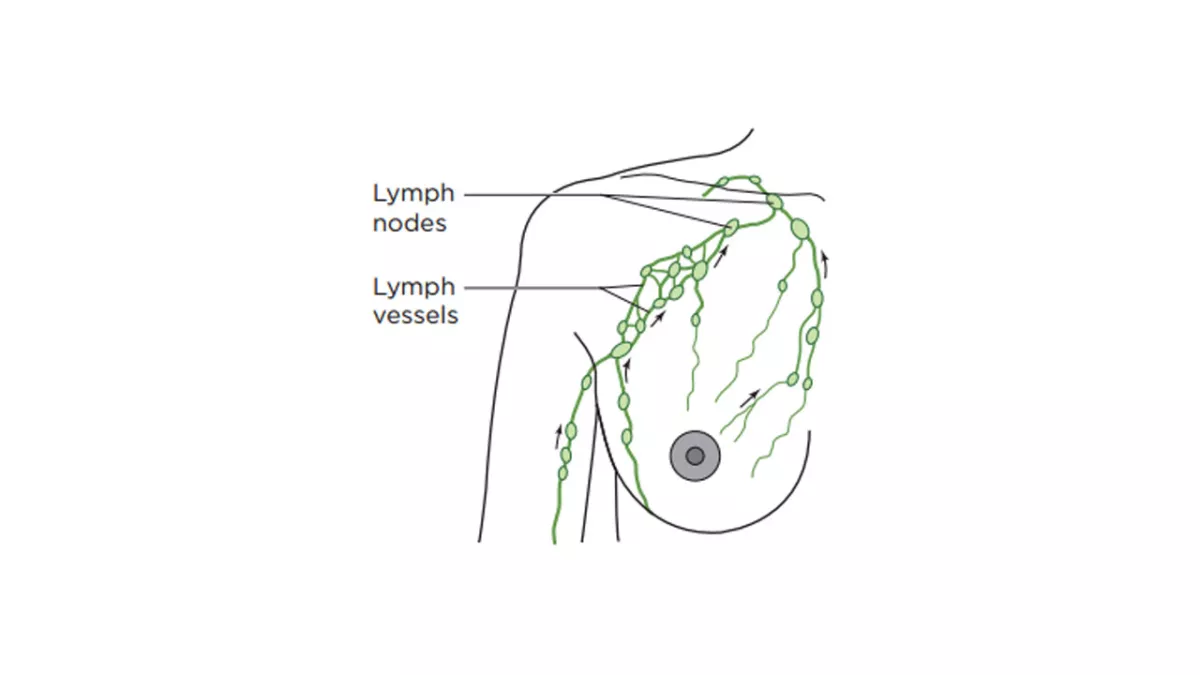
\includegraphics[width=\textwidth]{../figs/introduction/lymphatic_system_in_a_breast.png}
                        \caption{Lymphatic System Overview \cite{RefWorks:RefID:37-memorialsurgery}.}
                        \label{fig:introduction:lymphatic_system_in_a_breast}
                \end{subfigure}
                \begin{subfigure}[b]{0.45\textwidth}
                        \centering
                        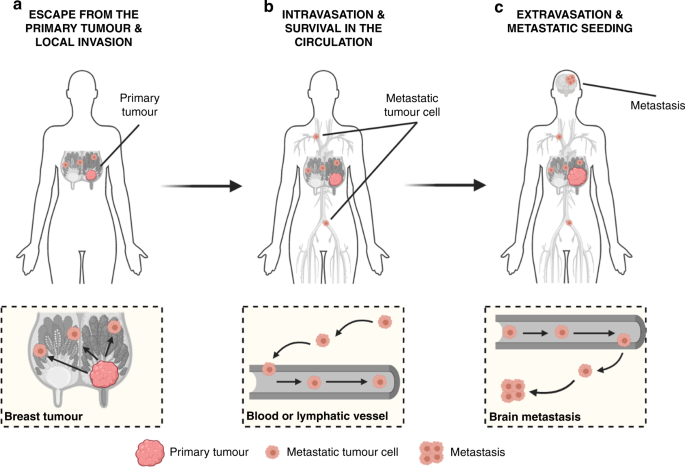
\includegraphics[width=\textwidth]{../figs/introduction/process_of_metastatic_breast_cancer.png}
                        \caption{Lymph Nodes Overview \cite{RefWorks:RefID:364-riggio2020lingering}.}
                        \label{fig:introduction:lymphatic_process_of_metastatic_breast_cancer}
                \end{subfigure}
        \end{minipage}
        \caption{Lymphatic System and Lymph Nodes Overview \cite{RefWorks:RefID:364-riggio2020lingering} \cite{RefWorks:RefID:37-memorialsurgery}.}
        \label{fig:introduction:lymphatic_system_and_nodes_overview}
\end{figure}

\subsection{Treatment of Breast Cancer\label{sec:introduction:treatmentofbreastcancer}}

\subsubsection{Stages of Breast Cancer\label{sec:introduction:breastcancer:stagesofbreastcancer}}
% Early vs late stage
Breast cancer is classified in stages ranging from 0 to IV based on the cancer's characteristics such as tumor size~\cite{RefWorks:RefID:151-2025breast}.

Stage 0 breast cancer is described as non-invasive, meaning the cancer cells are confined to the ducts or lobules in the breast and have not spread to surrounding healthy tissue~\cite{RefWorks:RefID:151-2025breast}.

Stage I breast cancer is invasive, meaning the cancer cells have spread to surrounding healthy tissue. In stage I breast cancer, the tumor is up to 2cm in size but invading cancer cells are no more than 1mm. Stage I is classified as either IA or IB depending on the sevarity of the cancer.~\cite{RefWorks:RefID:151-2025breast}.

Stage II breast cancer is used when the cancer is larger than 2cm but no larger than 5cm, or if the cancer has spread to one to three nearby lymph nodes. Similar to stage I breast cancer, stage II breast cancer can be subdivided into IIA and IIB~\cite{RefWorks:RefID:151-2025breast}.

Stage II breast cancer can be divided into IIIA, IIIB, and IIIC. This stage describes invasive breast cancer that is larger than 5cm or is found in four to nine nearby lymph nodes (IIIA), has spread to the chest wall or skin of the breast (IIIB), or has spread to ten or more nearby lymph nodes or to lymph nodes above or below the collarbone (IIIC)~\cite{RefWorks:RefID:151-2025breast}.

Lastly, stage IV breast cancer describes cancer that has metastasized, or spread, to other parts of the body such as the lungs, liver, bones, or brain~\cite{RefWorks:RefID:151-2025breast}.

Breast cancer stages can be divided into early and late stage breast cancer. Early-stage breast cancer incudes stages 0, I, and IIA while late-stage breast cancer includes stages IIB, III, and IV~\cite{RefWorks:RefID:365-stages}. Table~\ref{tab:introduction:breastcancer:stages} summarizes the stages of breast cancer. An overview of breast cancer treatment options for early and late stage breast cancer is shown in Figure~\ref{fig:introduction:breast_cancer_treatment_options_overview}.


\begin{table}[h!]
        \centering
        \caption{Stages of Breast Cancer~\cite{RefWorks:RefID:151-2025breast, RefWorks:RefID:365-stages}.}
        \label{tab:introduction:breastcancer:stages}
        \begin{tabular}{|c|c|c|}
                \hline
                \textbf{Stage} & \textbf{Description}                                       & \textbf{Early/Late Stage} \\
                \hline
                0              & Non-invasive, confined to ducts or lobules                 & Early                     \\
                \hline
                I              & Invasive, tumor up to 2cm, invading cells no more than 1mm & Early                     \\
                \hline
                IIA            & Tumor 2-5cm or spread to 1-3 lymph nodes                   & Early                     \\
                \hline
                IIB            & Tumor larger than 5cm or spread to 1-3 lymph nodes         & Late                      \\
                \hline
                IIIA           & Tumor larger than 5cm or found in 4-9 lymph nodes          & Late                      \\
                \hline
                IIIB           & Spread to chest wall or skin of breast                     & Late                      \\
                \hline
                IIIC           & Spread to 10+ lymph nodes or above/below collarbone        & Late                      \\
                \hline
                IV             & Metastasized to other parts of the body                    & Late                      \\
                \hline
        \end{tabular}
\end{table}

\subsubsection{Current Treatment Options\label{sec:introduction:breastcancer:currenttreatmentoptions}}

\subsubsection*{Surgical Options\label{sec:introduction:breastcancer:currenttreatmentoptions:surgicaloptions}}

Treatment options for breast cancer largely depend on the type and stage of the cancer. Surgical choices include a lumpectomy, which removes the tumor and a small margin of surrounding healthy tissue, or a mastectomy, which removes the entire breast~\cite{RefWorks:RefID:165-czajka2023breast}.

A lumpectomy is followed by radiation therapy to kill any stray cancer cells that may remain in the breast. This combination helps lower the risk of recurrence, or the return of the cancer~\cite{RefWorks:RefID:159-depolo2024radiation}. Radiation therapy is performed using high-energy X-rays to damage a cancer cell's DNA, preventing it from dividing further until it dies. Healthy tissue cells grow and divide slower than cancer cells, allowing them to repair themselves after radiation therapy while cancer cells cannot~\cite{RefWorks:RefID:159-depolo2024radiation}. See Section~\ref{sec:introduction:radiationtherapy} for more information on radiation therapy.

\subsubsection*{Lymph Node Biopsy\label{sec:introduction:breastcancer:currenttreatmentoptions:lymphnodebiopsy}}
In most surgical treatments for breast cancer, a lymph node biopsy is performed to check if cancer has spread past the breast tissue and to the lymph nodes. Samples from one or more lymph nodes are removed and examined under a microscope for cancer cells~\cite{RefWorks:RefID:37-memorialsurgery}. Standard practice was removing most of the lymph nodes in the underarm, called an axillary dissection. Today, a sentinel lymph node biopsy is more commonly performed to allow a faster recovery time~\cite{RefWorks:RefID:37-memorialsurgery}.

\subsubsection*{Sentinel Lymph Node Biopsy\label{sec:introduction:breastcancer:currenttreatmentoptions:sentinellymphnodebiopsy}}
The sentinel lymph node is the first lymph node that breast cancer cells spread to after leaving the breast. In a sentinel lymph node biopsy, a radioactive tracer (often technetium-99m) and/or a blue dye is injected into the side of the tumor. The tracer(s) travel through the lymphatic system to the sentinel lymph node. The blue stain and radiotracer signal, found with a gamma probe, can be used to identify and excise this lymph node for examination under a microscope for cancer cells~\cite{RefWorks:RefID:37-memorialsurgery},~\cite{RefWorks:RefID:165-czajka2023breast}.

\subsubsection*{Systemic Therapies\label{sec:introduction:breastcancer:currenttreatmentoptions:systemictherapies}}
While breast cancer treatment commonly starts with surgery, systemic therapies such as chemotherapy, hormone therapy, or targeted therapies may also be used~\cite{RefWorks:RefID:37-memorialsurgery}.

Chemotherapy, often called "chemo," uses strong medicines to slow or stop cancer cells from growing further. As chemotherapy often works by attacking cells that divide quickly, it can attack cancer cells but also other healthy cells that divide quickly such as those that make your hair grow. This can lead to side effects such as hair loss and nausea~\cite{RefWorks:RefID:37-memorialsurgery}.

Hormone treatment is used for breast cancer cells that require hormones such as estrogen to grow. This is done by blocking the hormones these cancer cells need to grow. Side effects can include changes in menstrual cycle, hot flashes, and aching bones~\cite{RefWorks:RefID:37-memorialsurgery}.

Targeted therapies, or precision medicines, attack specific characteristics of an individual's cancer cells rather than attacking all rapidly dividing cells like chemotherapy. Targeted therapies can treat the most common breast cancer gene mutations such as BRCA1 and BRCA2, HER2, and PIK3CA. This individualized treatment can lead to less side effects than in chemotherapy~\cite{RefWorks:RefID:37-memorialsurgery}.

\begin{figure}[h!]
        \centering
        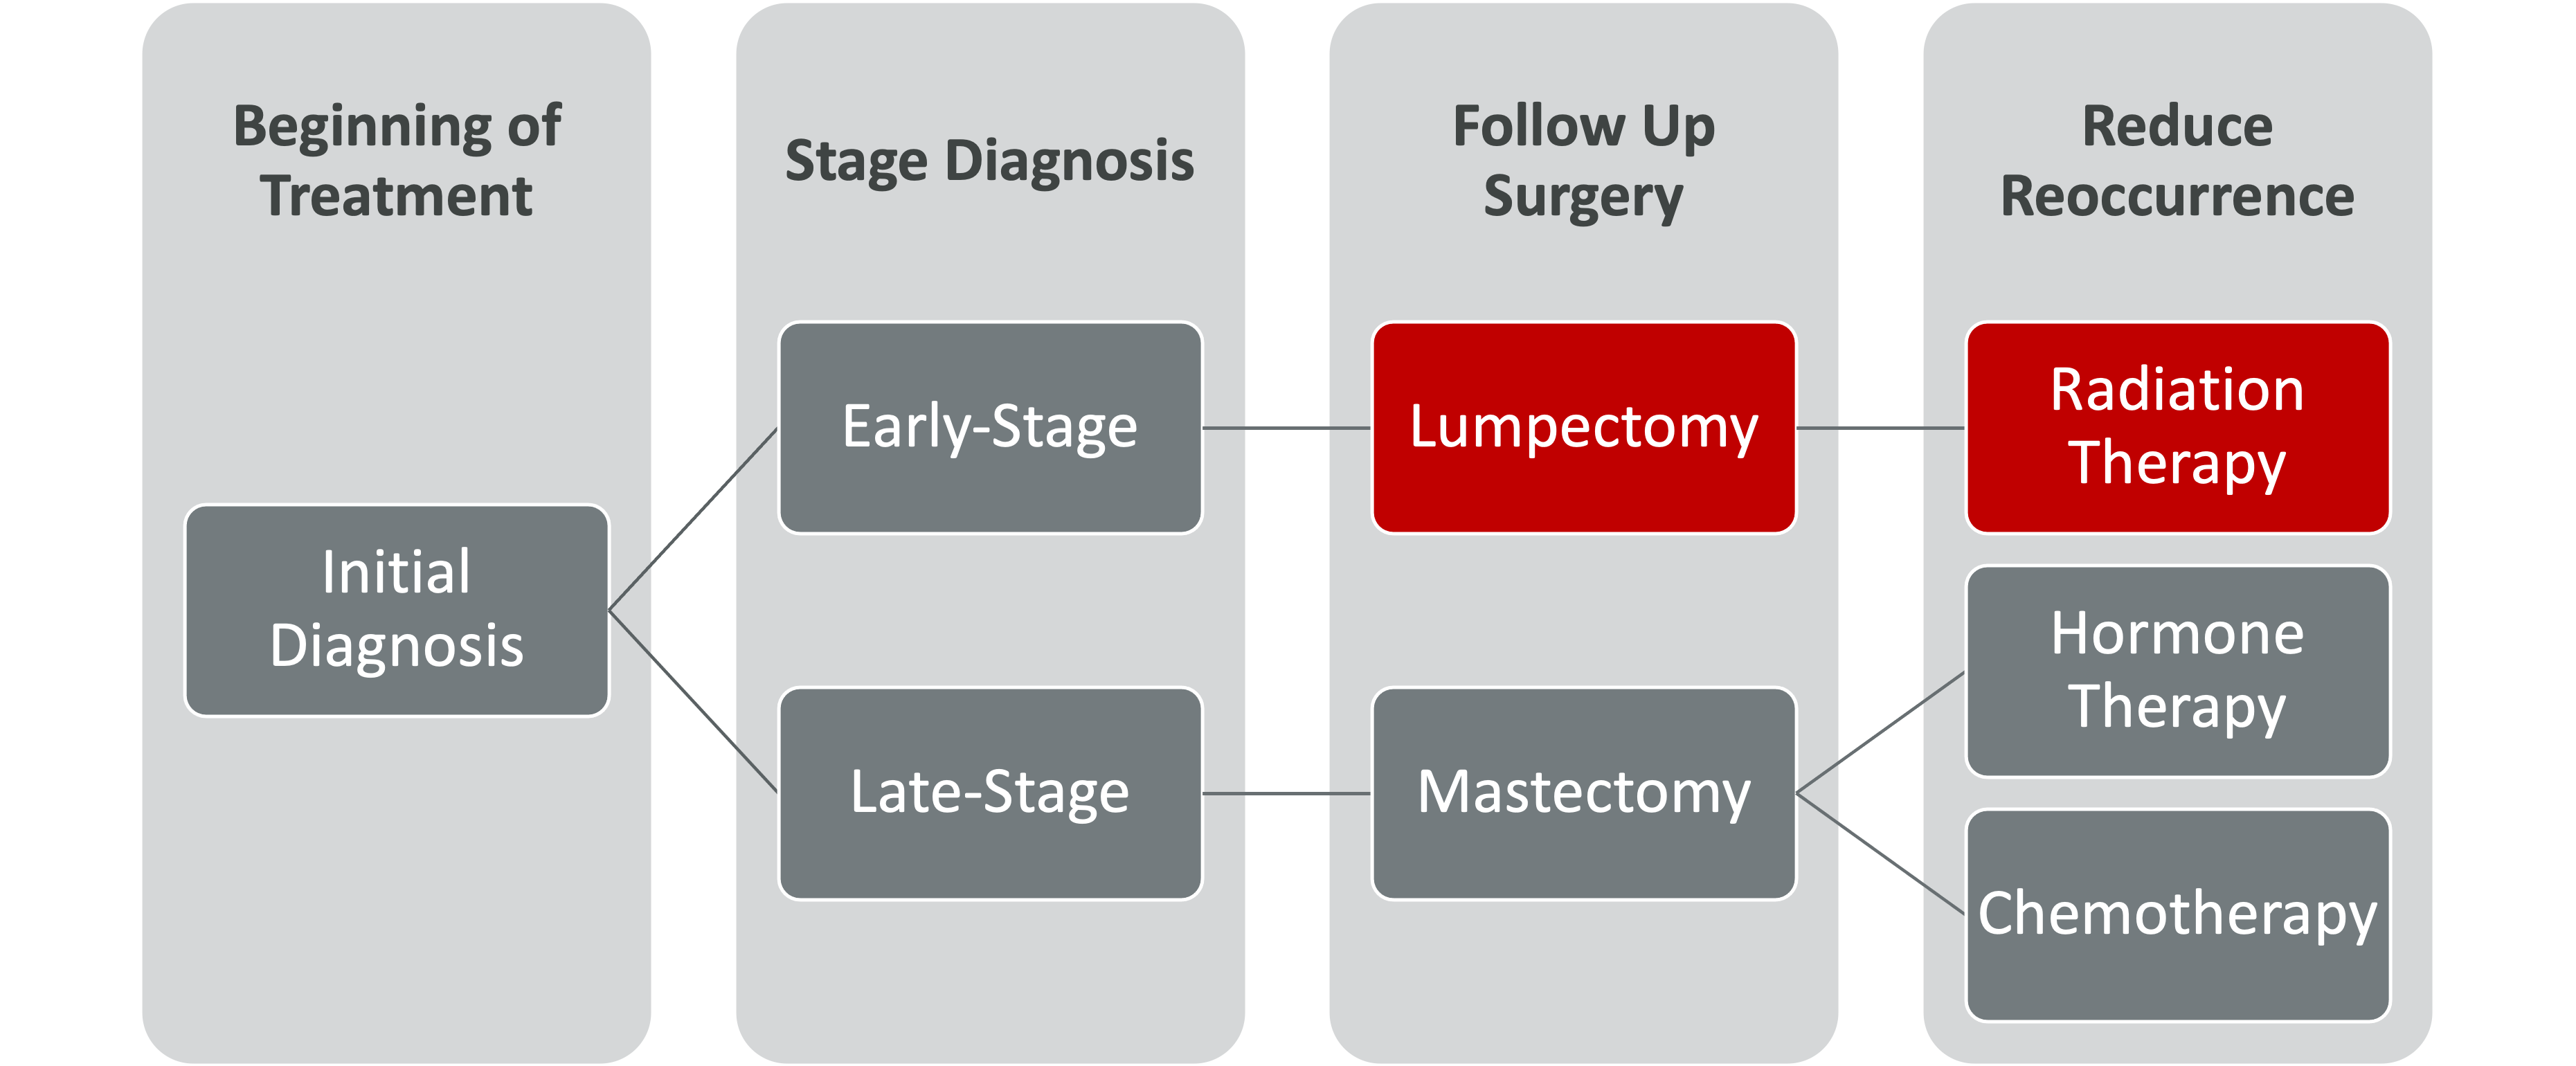
\includegraphics[width=0.6\textwidth]{../figs/introduction/breast_cancer_treatment_process_flowchart.png}
        \caption{Breast Cancer Treatment Options Overview \cite{RefWorks:RefID:37-memorialsurgery}, \cite{RefWorks:RefID:370-einsteinisaac}.}
        \label{fig:introduction:breast_cancer_treatment_options_overview}
\end{figure}

\subsection{Radiation Therapy\label{sec:introduction:radiationtherapy}}
\subsubsection{Radiation Therapy Overview\label{sec:introduction:radiationtherapy:overview}}
As mentioned in Section~\ref{sec:introduction:breastcancer:currenttreatmentoptions:surgicaloptions}, radiation therapy often follows a lumpectomy procedure to kill any stray cancer cells and prevent the cancer from resurfacing. Together, a lumpectomy procedure followed by radiation therapy is commonly known as breast-conserving therapy (BCT). Some compare breast cancer surgery to picking up the large pieces of a broken glass off the floor, while radiation therapy is like vacuuming the remaining shards at the end.

Including radiation therapy after a lumpectomy has been shown to reduce the risk of ipsilateral (same side) recurrence as well as increase overall survival rates~\cite{RefWorks:RefID:157-thomasscience}, ~\cite{RefWorks:RefID:198-jiao2024interobserver}.

\subsubsection{Whole vs Accelerated Partial Breast Irradiation\label{sec:introduction:radiationtherapy:wholevsacceleratedpartialbreastirradiation}}
Patients undergoing BCT can receive either whole breast irradation (WBI) or accelerated partial breast irradiation (APBI). WBI is the more common of the two techniques, although APBI has been gaining traction in recent years due to its unique benefits~\cite{RefWorks:RefID:157-thomasscience}.

WBI is delivered over the course of five to six weeks while APBI is delivered over the course of one week. APBI also limits radiation exposure to 1-2 cm margin of healthy tissue surrounding the tumor site. This limited exposure reduces radiation exposure risks to surrounding organs such as lungs, heart, or ribs. APBI also resulted in higher rates of "excellent/good" cosmetic outcomes compared to WBI (81\% vs 63\% respectively)~\cite{RefWorks:RefID:157-thomasscience}. Comparison of radiation exposure in WBI vs APBI is illustrated in Figure~\ref{fig:introduction:WBI_vs_APBI_irradiation_comparison}.

\begin{figure}[h!]
        \centering
        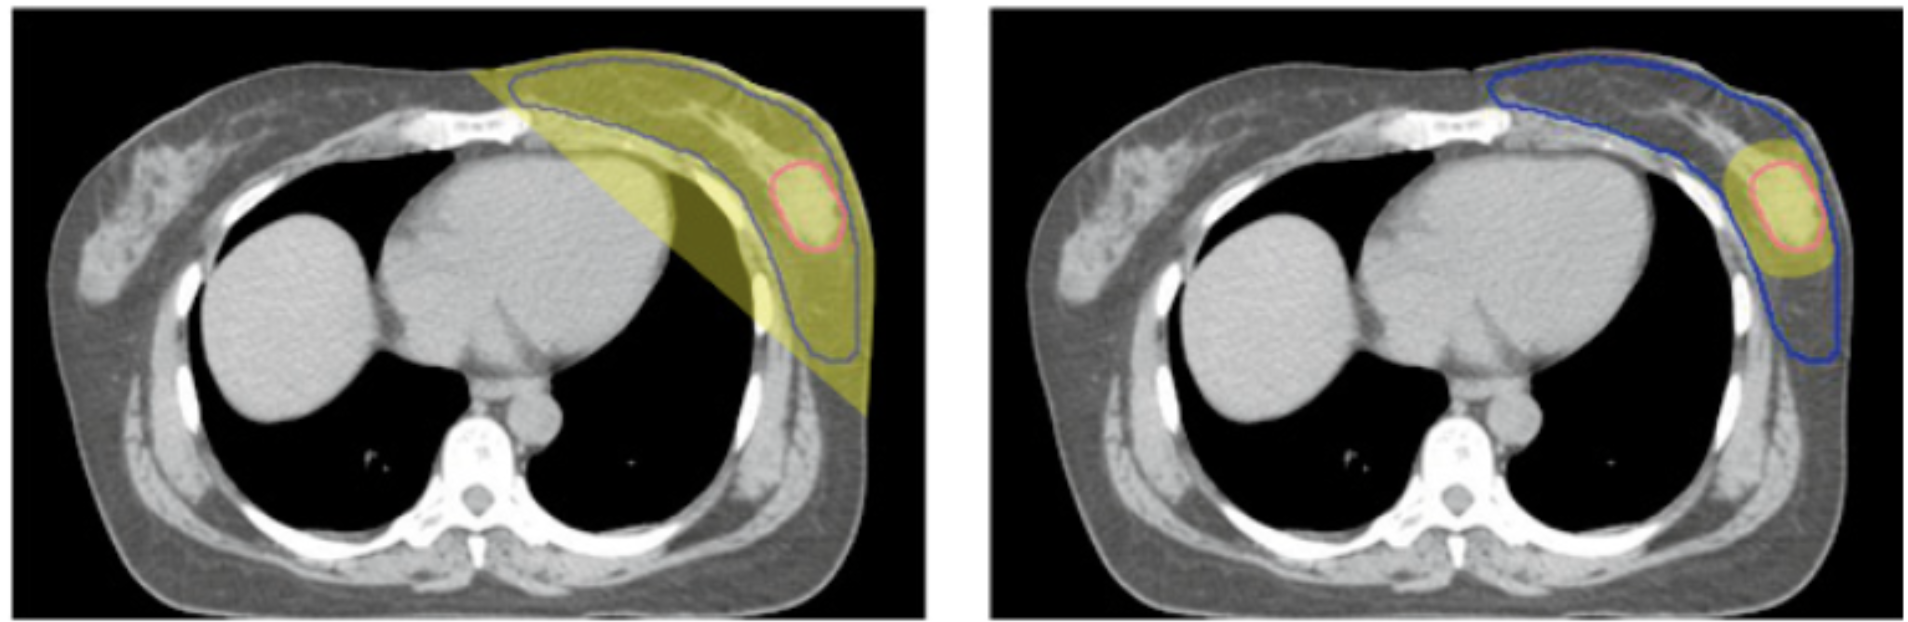
\includegraphics[width=0.6\textwidth]{../figs/introduction/WBI_vs_APBI_irradiation_comparison.png}
        \caption{Comparison of radiation exposure between Whole Breast Irradiation (WBI) (left) and Accelerated Partial Breast Irradiation (APBI) (right) \cite{RefWorks:RefID:157-thomasscience}. The yellow area indicates the irradiated region.}
        \label{fig:introduction:WBI_vs_APBI_irradiation_comparison}
\end{figure}

\subsubsection{Radiation Therapy Treatment Planning\label{sec:introduction:radiationtherapy:treatmentplanning}}
Radiation therapy (WBI or APBI) requires tumor bed delineation to identify and outline the tumor as well as a surrounding healthy tissue margin. This treatment planning ensures radiation is delivered accurately to the tumor site while minimizing exposure to healthy surrounding tissue and organs~\cite{RefWorks:RefID:197-den2015postlumpectomy}.

One concern with tumor bed (TB) delineation is the interobserver variability in accurately marking the TB~\cite{RefWorks:RefID:197-den2015postlumpectomy},~\cite{RefWorks:RefID:179-yang2013tumor}. There are many methods and devices used to assist in TB delineation to address these concerns such as surgical clips, pre-operative imaging, seroma formation, fiducial markers, and other implantable devices~\cite{RefWorks:RefID:179-yang2013tumor},~\cite{RefWorks:RefID:25-acree2022review}.

\subsection{Motivation\label{sec:introduction:motivation}}
The motivation for this work stems from the need to standardize and improve the accuracy and consistency of tumor bed (TB) delineation in radiation therapy following a lumpectomy procedure.

The challenges with accurate TB delineation following a lumpectomy procedure arise because the cancerous tissue has been removed, leaving behind a tumor cavity that is difficult to accurately trace~\cite{RefWorks:RefID:25-acree2022review}. Additionally, unlike other parts of the body, the breast lacks anatomic landmarks to assist with tumor bed delineation~\cite{RefWorks:RefID:344-mitchell2019adaptable}. This need for a marking method is visualized below in Figure~\ref{fig:introduction:need_for_tumor_bed_marker}.

\begin{figure}[h!]
        \centering
        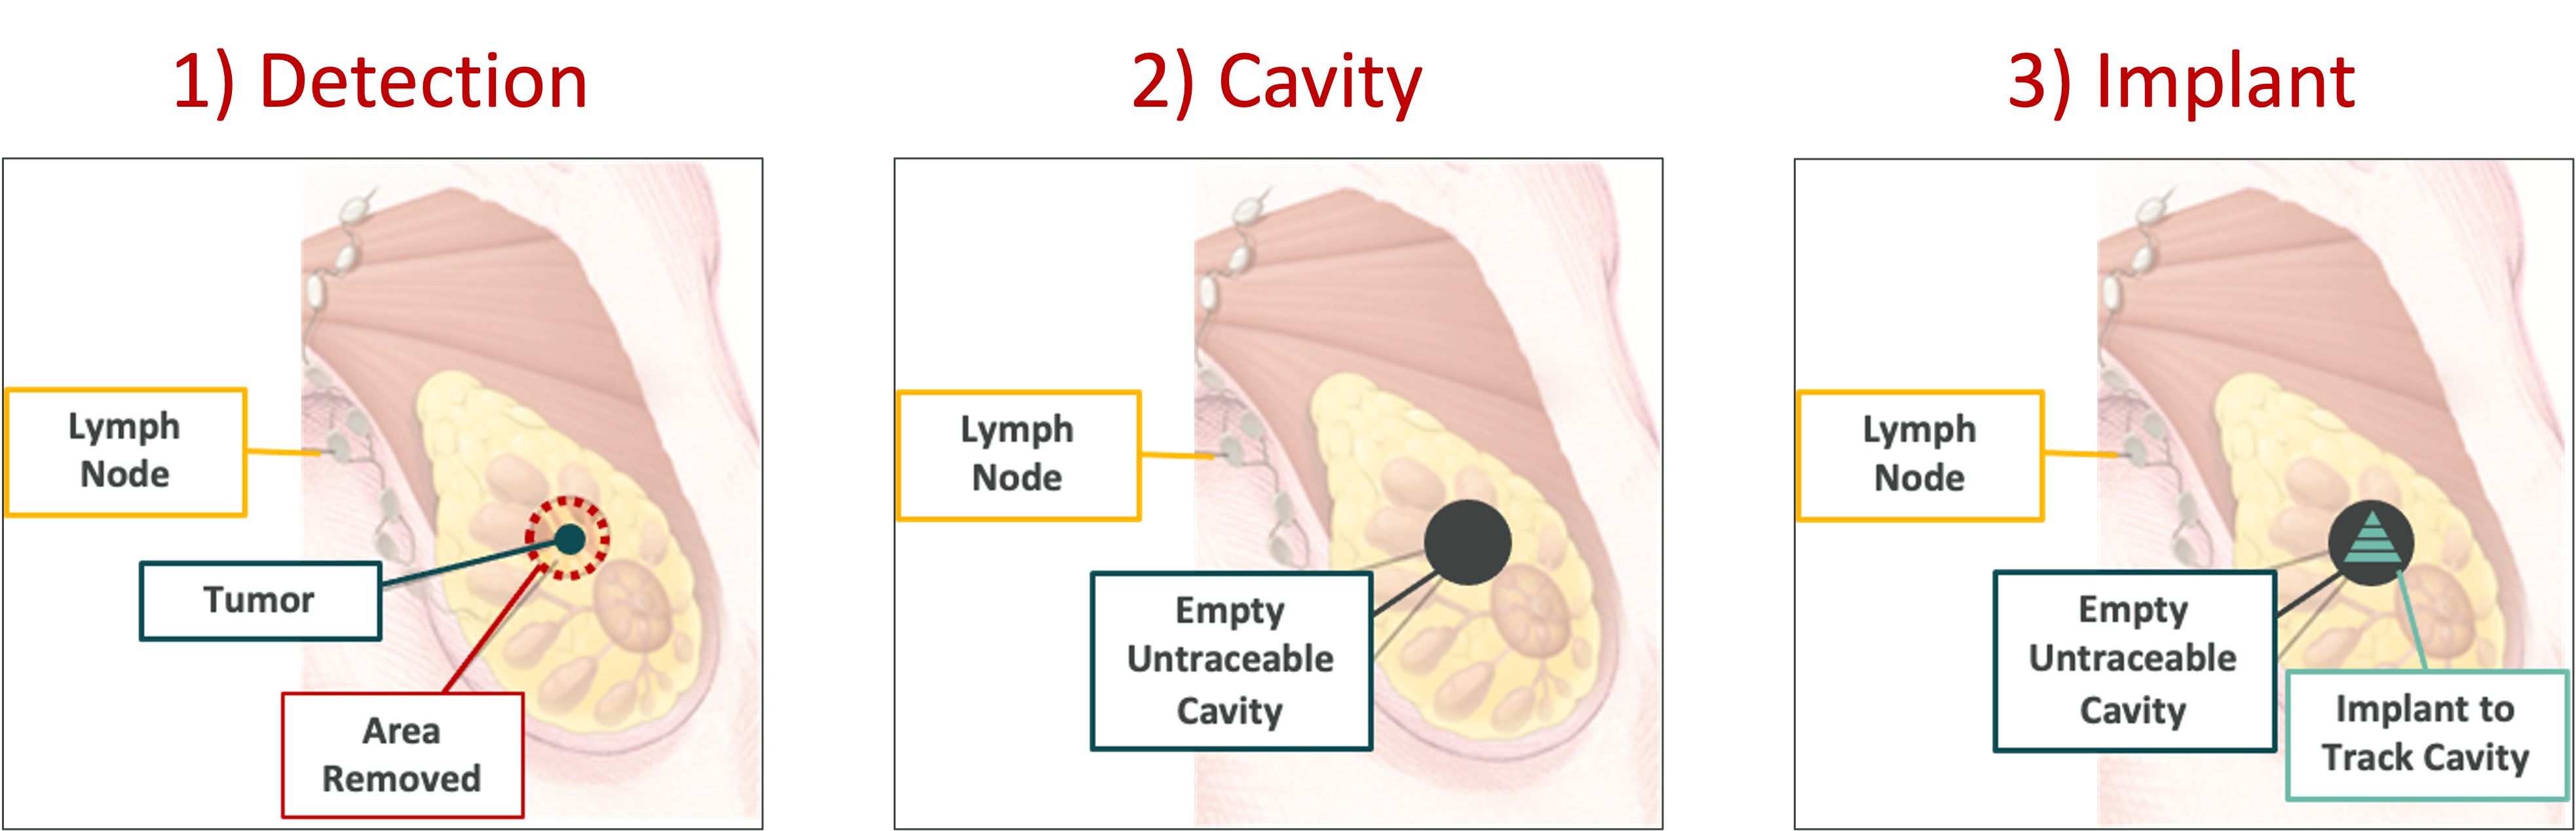
\includegraphics[width=0.6\textwidth]{../figs/introduction/need_for_tumor_bed_marker.png}
        \caption{Motivation for tumor cavity marker following lumpectomy procedure. Adapted from \cite{RefWorks:RefID:38-johnbreastconserving}.}
        \label{fig:introduction:need_for_tumor_bed_marker}
\end{figure}

Current devices and methods used for TB delineation have limitations that affect the overall consistency and accuracy of post-lumpectomy radiation therapy. As over 70\% of breast cancer recurrences occur at the original tumor site, accurate TB delineation and radiation delivery is important in improving patient outcomes~\cite{RefWorks:RefID:25-acree2022review}.

\subsubsection{Importance of Accurate Tumor Bed Delineation\label{sec:introduction:motivation:importanceofaccuratetumorbeddelineation}}
\hl{See if this could use more detail.\\}
Accurate TB delineation is crucial in effective radiation therapy following a lumpectomy procedure given the increasing use of APBI. Since APBI targets a small area of tissue surrounding the tumor bed, accurate delineation is necessary to ensure the radiation dose is delivered precisely to the intended area while minimizing exposure to surrounding healthy tissue and organs~\cite{RefWorks:RefID:197-den2015postlumpectomy}, ~\cite{RefWorks:RefID:25-acree2022review}.

Overestimating TB volume, common in seroma-based delineation, is associated with an increased risk of subcutaneous fibrosis and poorer cosmetic results~\cite{RefWorks:RefID:197-den2015postlumpectomy}. Conversely, underestimating TB volume can lead to insufficient radiation coverage of the tumor bed, increasing the risk of local recurrence~\cite{RefWorks:RefID:198-jiao2024interobserver}. An inaccurate TB volume can
also lead to alteration of management of a radiation boost and completely missing one or more margins of the TB~\cite{RefWorks:RefID:344-mitchell2019adaptable}.

\subsubsection{Current Devices and Methods\label{sec:introduction:motivation:currentdevicesandmethods}}
\hl{See if this could use more detail.\\}
Current devices and methods used for TB delineation include titanium, gold, or liquid fiducial markers/surgical clips, surgeon discretion, seroma formation, or implantable devices~\cite{RefWorks:RefID:25-acree2022review}.

Fiducial markers are solid metal clips inserted around the border of a tumor cavity immediately following the tumor removal~\cite{RefWorks:RefID:358-defining}. These provide a 2D point mapping of the tumor space as shown below in Figure~\ref{fig:introduction:imaging_of_fiducal_clips_in_phantom_breast}.

Liquid fiducial markers were first used as spacers for prostate cancer treatment planning. They have since been repurposed to be used for TB delineation. These markers provide a clearer delineation than solid clips as they conform to the tumor cavity shape~\cite{RefWorks:RefID:25-acree2022review}.

\begin{figure}[h!]
        \centering
        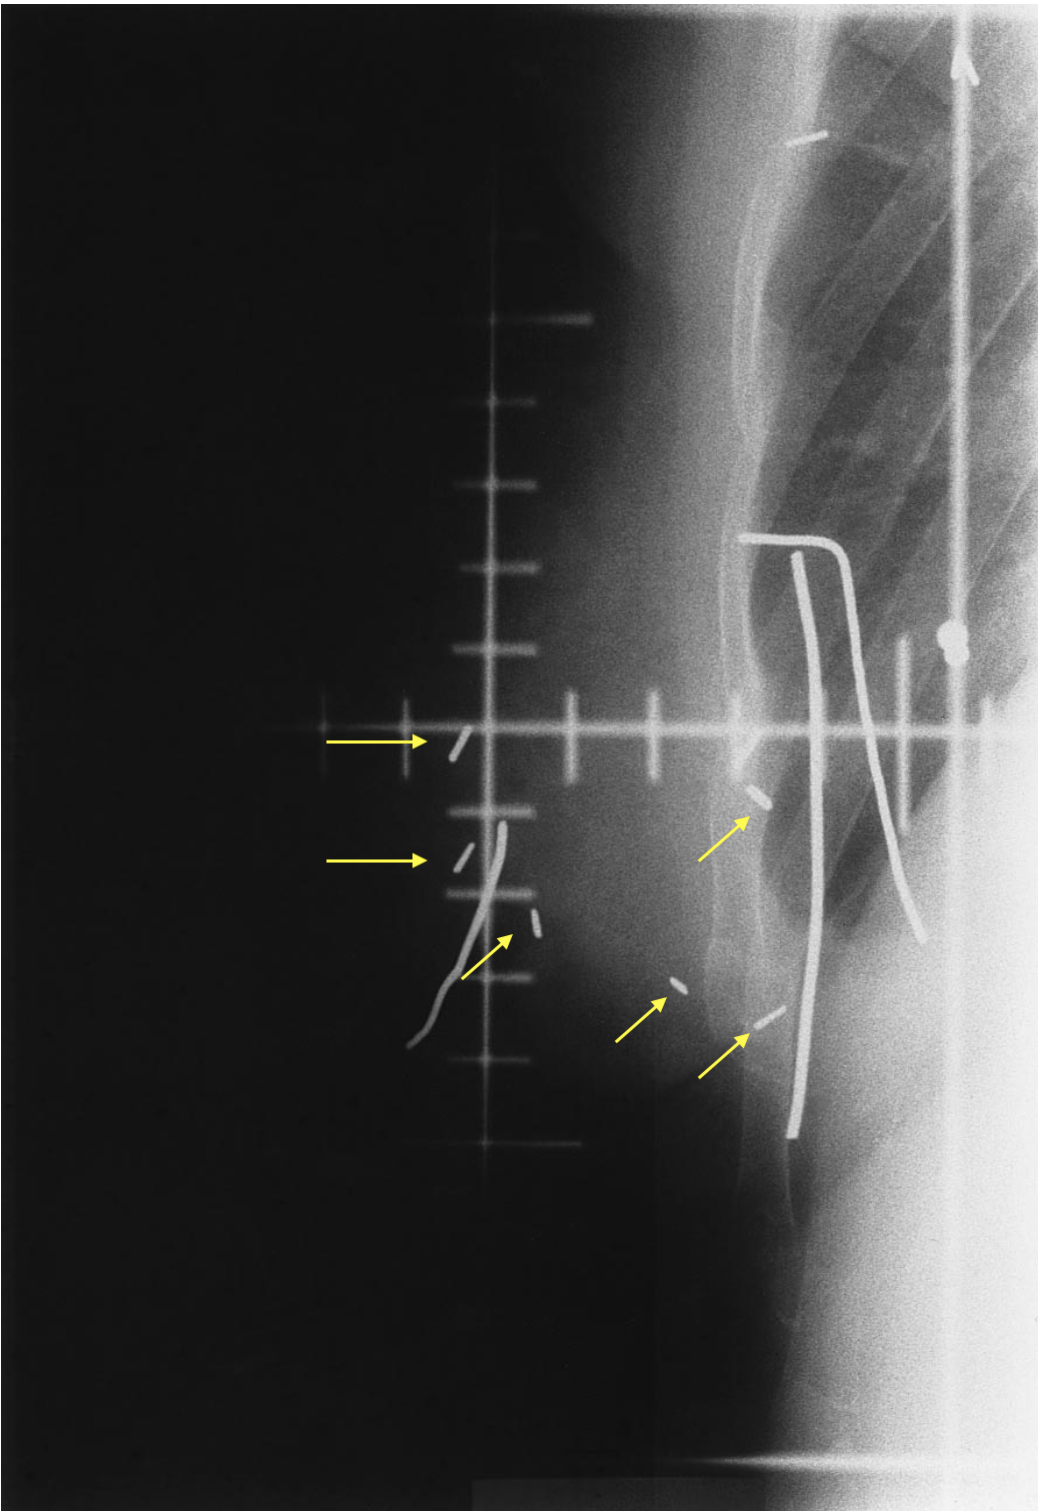
\includegraphics[width=0.6\textwidth]{../figs/introduction/imaging_of_fiducal_clips_in_phantom_breast.png}
        \caption{Imaging of Fiducial Clips in Phantom Breast. Yellow arrows indicate fiducial clips placed around tumor cavity. Adapted from \cite{RefWorks:RefID:178-krawczyk1994importance}.}
        \label{fig:introduction:imaging_of_fiducal_clips_in_phantom_breast}
\end{figure}

Using seroma formation to mark the tumor bed for radiation therapy involves outlining the seroma that forms following a lumpectomy procedure~\cite{RefWorks:RefID:25-acree2022review}.

Lastly, implantable devices can be used to mark the tumor bed. One example is BioZorb (Hologic) which is a 3-dimensional coil-like structure with titanium clips embedded. This device is implanted into the tumor cavity following a lumpectomy procedure and improves on titanium clips alone by creating a 3D outline of the tumor bed. BioZorb was also designed to be reabsorbed into the body within a year~\cite{RefWorks:RefID:25-acree2022review}. BioZorb is shown below in Figure~\ref{fig:introduction:biozorb_implant}.

\begin{figure}[h!]
        \begin{minipage}{0.92\textwidth}
                \centering
                \begin{subfigure}[b]{0.9\textwidth}
                        \centering
                        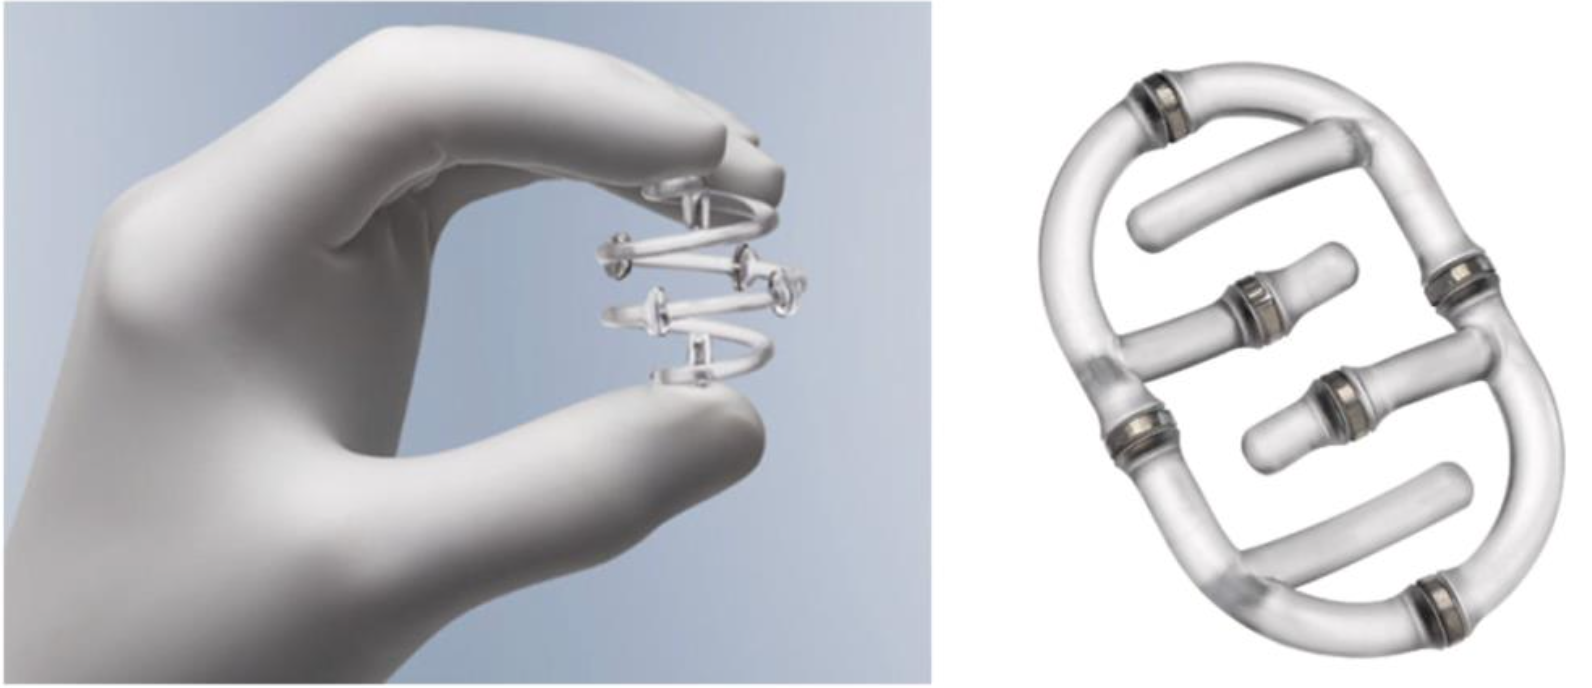
\includegraphics[width=\textwidth]{../figs/introduction/BioZorb_physically.png}
                        \caption{BioZorb physically (top).}
                        \label{fig:introduction:biozorb_physically}
                \end{subfigure}

                \vspace{1em} % optional space between images

                \begin{subfigure}[b]{0.9\textwidth}
                        \centering
                        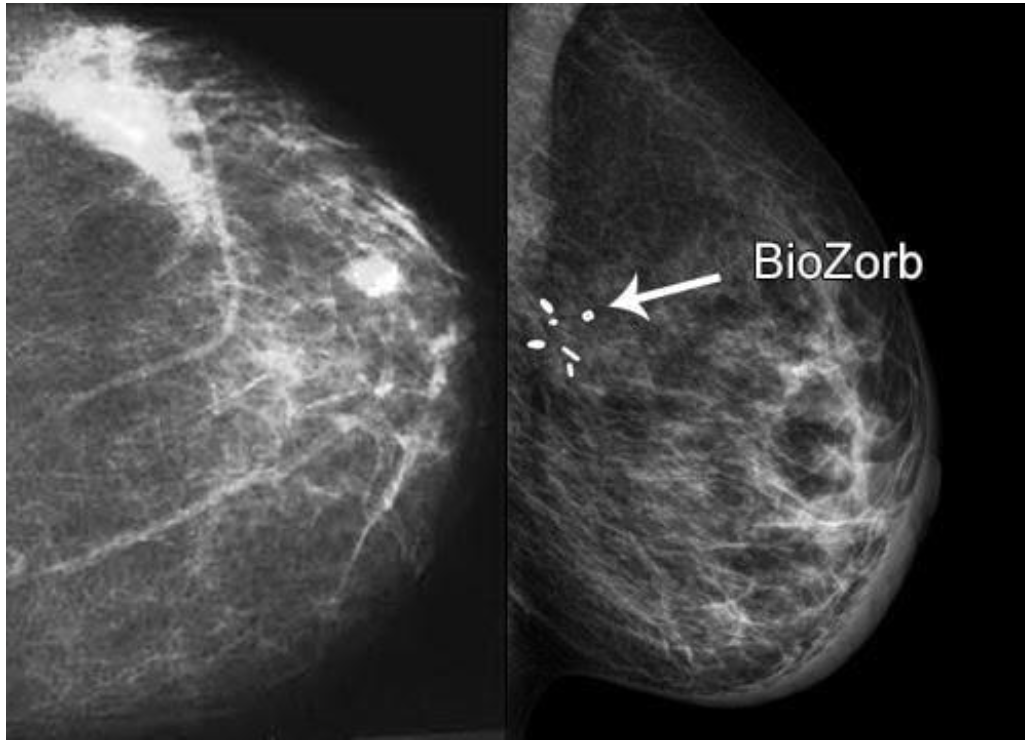
\includegraphics[width=\textwidth]{../figs/introduction/BioZorb_in_imaging.png}
                        \caption{BioZorb in imaging.}
                        \label{fig:introduction:biozorb_in_imaging}
                \end{subfigure}
        \end{minipage}
        \caption{BioZorb, an implantable device to assist with TB delineation~\cite{RefWorks:RefID:370-einsteinisaac}.}
        \label{fig:introduction:biozorb_implant}
\end{figure}

A newer implantable device is Veraform, a continuously radiographically opaque filament that is stitched around the tumor cavity. By being malleable and sewn in place, this device addresses space limitations and migration issues present in other devices~\cite{RefWorks:RefID:344-mitchell2019adaptable}. A simulation showing Veraform in use is shown below in Figure~\ref{fig:introduction:veraform_implant}.
\begin{figure}[h!]
        \centering
        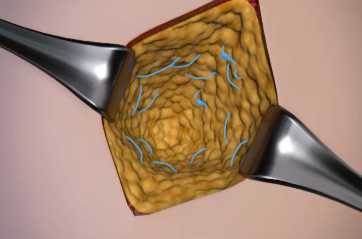
\includegraphics[width=0.6\textwidth]{../figs/introduction/veraform_implant.png}
        \caption{Veraform, an implantable device to assist with TB delineation~\cite{RefWorks:RefID:344-mitchell2019adaptable}.}
        \label{fig:introduction:veraform_implant}
\end{figure}

\subsubsection{Challenges with Current Devices and Methods\label{sec:introduction:motivation:challengeswithcurrentdevicesandmethods}}
\hl{See if this could use more detail.\\}

\subsubsection*{Challenges with Fiducial Markers\label{sec:introduction:motivation:challengeswithcurrentdevicesandmethods:challengeswithfiducialmarkers}}
There are many challenges and inaccuracies that can result from using fiducial markers or surgical clips to create a TB volume. They provide single points of reference which can lead to inaccurate boundaries being drawn, there is no standardized recommendation of how many clips should be used, and clips can migrate over time leading to inaccurate TB localization~\cite{RefWorks:RefID:344-mitchell2019adaptable}. Migration is especially common when patients undergo oncoplastic reconstruction surgery following the lumpectomy procedure. In 2022, it was found the 30,000 breast-conserving therapy patients annually undergo oncoplastic reconstruction surgery~\cite{RefWorks:RefID:25-acree2022review}.

Another concern of surgical clips or fiducial markers is if a re-excision is required. This is when a margin of tissue removed during the lumpectomy is found to contain cancerous cells. When this is the case, a large enough margin surrounding the tumor was not removed, and a re-excision has to be made to remove additional margins. When markers are placed initially, these re-excisions can impact the accuracy of the initial marker placement. It was found that 10\% to 20\% of patients undergoing breast-conserving surgery require a re-excision~\cite{RefWorks:RefID:25-acree2022review}.

\subsubsection*{Challenges with Seroma Formation\label{sec:introduction:motivation:challengeswithcurrentdevicesandmethods:challengeswithseromaformation}}
\hl{Show change in seroma over time visual.\\}

Utilizing seroma formation can be unreliable, as the seroma may not always be localized to the tumor bed, relies on the excision closure method, and time elapsed after surgery\cite{RefWorks:RefID:25-acree2022review}. A seroma may represent the tumor bed, part of the tumor bed, or the entire area in which surgery was performed~\cite{RefWorks:RefID:344-mitchell2019adaptable}.

\subsubsection*{Challenges with Biozorb}
Biozorb was found to provide limited value to patients relative to its high cost~\cite{RefWorks:RefID:344-mitchell2019adaptable}. Additionally, Biozorb was also recalled due to patient discomfort, seroma formation, device migration, and failures to resorb into the body in the designated timeframe~\cite{RefWorks:RefID:296-2024hologic},~\cite{RefWorks:RefID:28-nudelunited}.

\subsubsection{Proposed Solution\label{sec:introduction:motivation:proposedsolution}}
% Explain our research and the proposed mesh


\section{Prior Work Completed\label{introduction:priorWork}}

This project idea of an improved lumpectomy tumor bed marking method was first proposed by the Division Chief for Oncoplastic Surgery at The Ohio State University Comprehensive Cancer Center (OSUCCC), Dr. Roman Skoracki~\cite{RefWorks:RefID:372-krakovskytumor},~\cite{RefWorks:RefID:371-bakhtardesign}.

This project was then adopted bya mechanical engineering senior capstone in 2022 (\hl{Check this date}). It has since been further explored by Adrian Bakhtar, Isaac Einstein, and Zuhaib Jama. The general contributions of each group are summarized below in Table~\ref{tab:introduction:priorWorkCompletedOverview}.

\begin{table}[H]
        \centering
        \caption{Summary of Prior Team and Researcher Contributions}
        \label{tab:introduction:priorWorkCompletedOverview}
        \begin{tabularx}{\textwidth}{>{\raggedright\arraybackslash}p{3cm} X >{\raggedright\arraybackslash}p{3cm}}
                \toprule
                \textbf{Team/Researcher}                                       & \textbf{General Contribution(s)} & \textbf{Time Working on Project} \\
                \midrule
                Senior Capstone Group~\cite{RefWorks:RefID:372-krakovskytumor} &
                - Identified initial pain points and opportunity \newline
                - Evaluated various end-product concepts \newline
                - Selected ideal form factor and developed initial device prototype
                                                                               & 2022                                                                \\
                \addlinespace
                Adrian Bakhtar~\cite{RefWorks:RefID:371-bakhtardesign}         &
                - Continued work started by senior capstone team \newline
                - Worked with stakeholders to refine device design \newline
                - Optimized device geometry, printability, and adhesive capabilities \newline
                - Defended master's thesis and is continuing research through a PhD
                                                                               & 2022 -- Present                                                     \\
                \addlinespace
                Zuhaib Jama~\cite{RefWorks:RefID:384-jamacomputational}        &
                - Evaluated potential stresses experienced by the device via FEM \newline
                - Presented findings at research poster symposium
                                                                               & 2024                                                                \\
                \addlinespace
                Isaac Einstein~\cite{RefWorks:RefID:370-einsteinisaac}         &
                - Evaluated material properties of device base material \newline
                - Presented findings through a research poster symposium and undergraduate thesis
                                                                               & 2023 -- 2024                                                        \\
                \bottomrule
        \end{tabularx}
\end{table}

\subsection{Senior Capstone Work\label{sec:introduction:priorWork:seniorCapstone}}

\subsubsection{Device Requirements\label{sec:introduction:priorWork:seniorCapstone:deviceRequirements}}
Working alongside the OSUCCC including surgeons, radiation oncologists, and dosimetrists, the senior capstone team developed target functional requirements for the device. This is outlined below in Table~\ref{tab:introduction:priorWork:seniorCapstone:targetSpecifications}.

\begin{table}[H]
        \centering
        \caption{Initial Device Target Specifications~\cite{RefWorks:RefID:372-krakovskytumor},~\cite{RefWorks:RefID:371-bakhtardesign}}
        \label{tab:introduction:priorWork:seniorCapstone:targetSpecifications}
        \begin{tabularx}{\textwidth}{
                >{\centering\arraybackslash}p{1.2cm}
                >{\raggedright\arraybackslash}p{3.5cm}
                X
                }
                \toprule
                \textbf{Weight} & \textbf{Specification} & \textbf{Requirement} \\
                \midrule
                1               & Biocompatibility       &
                Follows ISO 10993 \newline
                • Twenty-part protocol FDA testing process                      \\
                \addlinespace
                2               & Sterilizable           &
                Follows ISO 11135 \newline
                • Sterilization of health-care products (Ethylene oxide) \newline
                Packaging follows ISO 11607 \newline
                • Packaging for sterilized material                             \\
                \addlinespace
                3               & Implantation speed     &
                < 3 minutes                                                     \\
                \addlinespace
                4               & Radiodensity           &
                > 0 HU and < 3000 HU (Hounsfield Units)                         \\
                \addlinespace
                5               & Longevity              &
                6 weeks -- 12 months                                            \\
                \addlinespace
                6               & Mechanical Properties  &
                812 -- 4500 kg/m\textsuperscript{3}                             \\
                \addlinespace
                7               & Size/Area              &
                2 -- 7 cm in diameter \newline
                10 -- 150 cm\textsuperscript{2}                                 \\
                \addlinespace
                8               & Cost                   &
                < \$1250                                                        \\
                \bottomrule
        \end{tabularx}
\end{table}

Because the device would eventually be implanted in human patients, biocompatibility and sterilization were given the highest importance. Implantation speed was next based on surgeon feedback~\cite{RefWorks:RefID:372-krakovskytumor}.

It was believed the chances of device adoption by surgeons would decrease if implantation speed was significant~\cite{RefWorks:RefID:372-krakovskytumor}.

Discussions with dosimetrists led the group to select a target Hounsfield Units (HU) of less than 3,000 HU to reduce radiation reflection and provide adequate contrast from breast tissue~\cite{RefWorks:RefID:372-krakovskytumor}.

The longevity of the device was estimated through conversations with OSUCCC based on the range of lumpectomy procedure timelines~\cite{RefWorks:RefID:372-krakovskytumor}.

The mechanical properties were selected to mirror breast tissue based on additional team research~\cite{RefWorks:RefID:372-krakovskytumor}.

Lastly, the size and cost of the device were selected based on research into existing competitor devices~\cite{RefWorks:RefID:372-krakovskytumor}.

\subsubsection{Initial Prototype Development\label{sec:introduction:priorWork:seniorCapstone:initialPrototypeDevelopment}}

\paragraph*{Material Selection\label{sec:introduction:priorWork:seniorCapstone:initialPrototypeDevelopment:materialSelection}}
To adhere with the mechanical properties and biodegradable needs of the device, the capstone team selected Poly(l-lactide-co-$\varepsilon$-caprolactone) (PLCL) as the base material. This is a biodegradable and biocompatible material with an adjustable degredation timeline and mechanical properties. It is composed of two co-polymers: Polylactic acid (PLA) and Polycaprolactone (PCL). The radiopaque agent selected was barium sulfate (BaSO4) based on its extensive clinical trials and current use in digestive marking~\cite{RefWorks:RefID:372-krakovskytumor}.

\paragraph*{Device Form Factor\label{sec:introduction:priorWork:seniorCapstone:initialPrototypeDevelopment:formFactor}}
As shown in Figure~\ref{fig:introduction:initialCapstonePrototype}, the capstone team designed the device in a hemispherical and collapsible form factor. The team created the prototype through melting base materials into a premade mold~\cite{RefWorks:RefID:372-krakovskytumor}.

\paragraph*{Imaging Testing\label{sec:introduction:priorWork:seniorCapstone:initialPrototypeDevelopment:imaginTesting}}

Imaging capabilities and radiopacity of the initial prototype was evaluated by the capstone team to evaluate the desired amount of barium sulfate. This initial testing resulted in excessively bright samples, which illustrated the need to minimal barium sulfate addition~\cite{RefWorks:RefID:372-krakovskytumor}. The capstone team's imaging testing is shown below in Figure~\ref{fig:introduction:capstoneImagingTesting}.

\begin{figure}[h!]
        \centering
        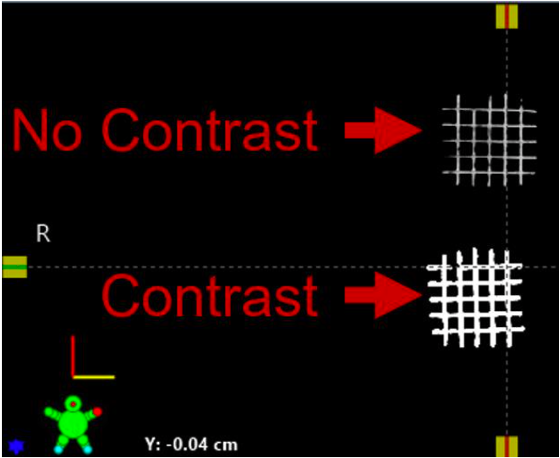
\includegraphics[width=0.8\textwidth]{../figs/introduction/capstone_imaging_testing.png}
        \caption{Initial imaging results from senior capstone team~\cite{RefWorks:RefID:372-krakovskytumor}.}
        \label{fig:introduction:capstoneImagingTesting}
\end{figure}

\subsubsection{Future Questions\label{sec:introduction:priorWork:seniorCapstone:futureQuestions}}

The senior capstone, while making strides in the early development of the device, had areas that could benefit from additional testing. This includes focusing on optimizing the manufacturing process, making the overall mesh thinner, decreasing the amount of barium sulfate embedded, and performing longer-term biodegradability testing.

\subsection{Additional Research Team Work\label{sec:introduction:priorWork:otherTeamWork}}

\subsubsection{Design of Device\label{sec:introduction:priorWork:otherTeamWork:deviceDesign}}

Culminating in the successful defense of a master's thesis, Adrian Bakhtar spearheaded the overall design of the device~\cite{RefWorks:RefID:371-bakhtardesign}.

\paragraph*{Device Geometry\label{introduction:priorWork:otherTeamWork:deviceDesign:deviceGeometry}}

It was initially anticipated that the device geometry would be patient specific based on each unique tumor volume. Based on stakeholder and end-user feedback, it was determined that this approach would not be feasible given the high cost, implementation time, and differences between pre- and post-surgery tumor shapes (See Section~\ref{sec:introduction:priorWork:otherTeamWork:customerDiscovery} for more information).

Given this change, the device was converted from a patient-specific geometry to a uniform mesh with a thickness of 0.125mm. This mesh is shown below in Figure~\ref{fig:introduction:initialThinMeshDesign}. The minimal profile of this mesh allows it to be flexible and easily cuttable by surgeons. Additionally, triangular  cutouts were added to provide directional orientation for radiation oncologists when creating treatment plans. The mesh sheets were created in 20 x 20$mm^2$ and 38 x 38$mm^2$ squares to adequately cover traditional tumor sizes~\cite{RefWorks:RefID:371-bakhtardesign}.

\begin{figure}[h!]
        \centering
        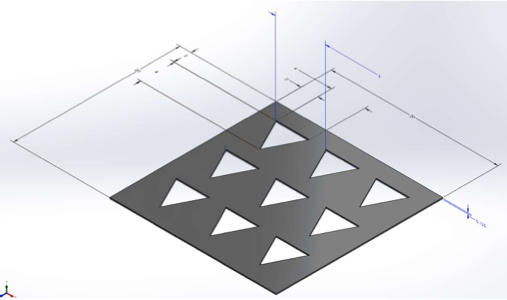
\includegraphics[width=0.8\textwidth]{../figs/introduction/thin_flat_mesh_design_with_cutouts.png}
        \caption{Refined thin mesh design with directional cutouts~\cite{RefWorks:RefID:371-bakhtardesign}.}
        \label{fig:introduction:initialThinMeshDesign}
\end{figure}

\paragraph*{Surface Texture\label{introduction:priorWork:otherTeamWork:deviceDesign:surfaceTexture}}

The mesh design needed to be fixed in place to address the concern of migration seen by existing devices like fiducial clips~\cite{RefWorks:RefID:344-mitchell2019adaptable}. The initial capstone team planned to secure the mesh to the tumor bed walls via suturing, though this could increase the implementation time substantially~\cite{RefWorks:RefID:372-krakovskytumor}. To address this adhesion concern, a texture was added to the top of the flat mesh to grab onto and increase friction between the mesh and tissue. Using the SolidWorks built in "Treadplate Bump" feature, a 3 x 3 mm treadplate bump with a texture offset of 0.75 mm and maximum element size of 0.125 mm was applied to the initial mesh~\cite{RefWorks:RefID:371-bakhtardesign}. This is shown below in Figure~\ref{fig:introduction:meshWithTreadplate}.

\begin{figure}[h!]
        \centering
        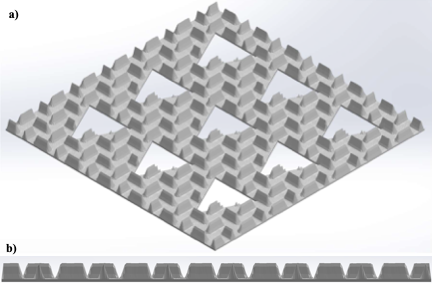
\includegraphics[width=0.8\textwidth]{../figs/introduction/mesh_design_with_treadplate.png}
        \caption{Isometric (a) and front view (b) of thin mesh design with treadplate bump appliedRefined thin mesh design with directional cutouts~\cite{RefWorks:RefID:371-bakhtardesign}.}
        \label{fig:introduction:meshWithTreadplate}
\end{figure}

\paragraph*{Friction and Implantation Testing\label{introduction:priorWork:otherTeamWork:deviceDesign:frictionTesting}}
To test the efficacy of the added surface texture, a friction test was performed. This test evaluated various texture and mesh geometry settings. The friction testing helped inform the device design by illustrating that a higher offset height and larger treadplate features yielded a higher static coefficient of friction.

The mock implantation testing, performed using raw chicken breast, showed that the textured mesh adhered closely to the cavity walls following excessive force and handling of the chicken breast. Both of these test setups are illustrated below in Figure~\ref{fig:introduction:frictionAndImplantationTesting}.

\begin{figure}[h!]
        \centering
        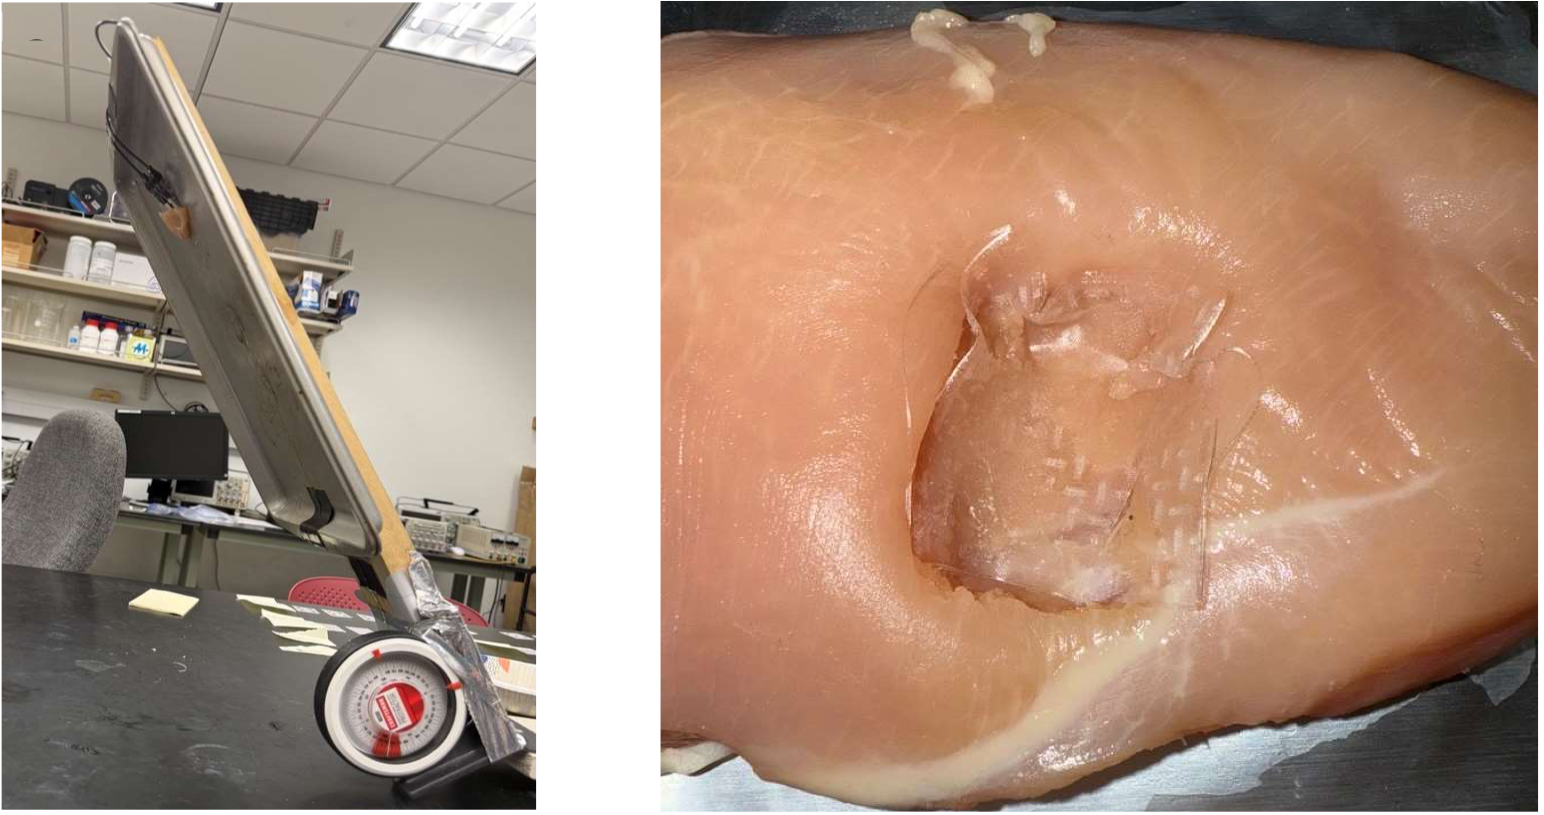
\includegraphics[width=0.8\textwidth]{../figs/introduction/friction_and_implantation_testing.png}
        \caption{Friction testing (left) and implantation testing (right)~\cite{RefWorks:RefID:371-bakhtardesign}.}
        \label{fig:introduction:frictionAndImplantationTesting}
\end{figure}


\subsubsection{Biodegradability Evaluation\label{sec:introduction:priorWork:otherTeamWork:biodegradabilityEval}}

Expanding on the capstone team's initial testing, a long-term biodegradability test was performed on the base material, PLCL. This degradation study used thin mesh squares to evaluate degradation timeline between 1 and 7 months at 37\textdegree C. While this study is still ongoing, one-month results showed an average mass loss of 0.071$\frac{gram}{month}$~\cite{RefWorks:RefID:371-bakhtardesign}.

\subsubsection{Initial Imaging Testing}

To help inform the device design, specifically the internal printing parameters of the device, initial imaging testing was performed on PLCL, PCL, PLA, and PLGA-HA filaments. The effects on radiopacity of infill density, infill pattern, sample height, and sample composition were evaluated through this imaging study.

It was found that PLCL, PCL, and PLA were essentially indistinguishable from one another, while PLGA-HA was marginally brighter. Limitations on this study resulted from the size of samples and subsequent resolution of results. In the future, larger samples may help draw clearer radiopacity conclusions~\cite{RefWorks:RefID:371-bakhtardesign}.

\subsubsection{3D Printing Work\label{sec:introduction:priorWork:otherTeamWork:3dPrinting}}

\paragraph*{Optimizing PLCL Printing Parameters\label{sec:introduction:priorWork:otherTeamWork:3dPrinting:plclParameters}}

While development of a custom PLCL 3D printable filament was underway, externally sourced PLCL filament was bought for mechanical testing and improvement of device design. 1.75mm filament was bought from Lattice Medical, a French-based company~\cite{RefWorks:RefID:42-latticemedical}.

Fused deposition modeling (FDM) printing was conducted with this filament (see Section~\ref{chap:literatureReview}\hl{Update \# after adding 3D printing section} for additional information on FDM printing).

Necessary printing parameters, including nozzle temperature, bed temperature, layer height, infill density, and print speed, needed to be adjusted and optimized for the Lattice PLCL filament. Multiple line tests and scaled device prints were preformed to manually optimize the printing parameters for this filament. The optimal parameters are shown below in Table~\ref{tab:introduction:priorWork:plclPrintingParameters}~\cite{RefWorks:RefID:371-bakhtardesign}. These tests were conducted using a Prusa i3 MK3 printer.

\begin{table}[h!]
        \centering
        \caption{Optimal Printing Parameters for Lattice PLCL on Prusa i3 MK3 Printer}
        \label{tab:introduction:priorWork:plclPrintingParameters}
        \begin{tabularx}{0.8\textwidth}{
                >{\raggedright\arraybackslash}p{5cm}
                >{\raggedright\arraybackslash}X
                }
                \toprule
                \textbf{Parameter}                  & \textbf{Optimal Value} \\
                \midrule
                First layer print speed             & 20 mm/s                \\
                First layer nozzle temperature      & 180\,\textdegree C     \\
                Subsequent layer nozzle temperature & 190\,\textdegree C     \\
                Bed temperature                     & 30\,\textdegree C      \\
                Infill density                      & 10\%                   \\
                \bottomrule
        \end{tabularx}
\end{table}

% a.	Optimizing PLCL printing parameters
% b.	Layer shape

\subsubsection{Customer Discovery\label{sec:introduction:priorWork:otherTeamWork:customerDiscovery}}
% a.	I-Corps
% i.	Led to thin sheet instead of patient-specific shape

\subsection{Undergraduate Thesis\label{sec:introduction:priorWork:undergradThesis}}

\subsubsection{Felfil Extrusion Work\label{sec:introduction:priorWork:undergradThesis:felfil}}
% Trying to extrude a powder unsuccessfully

\subsubsection{Mechanical Testing of Lattice PLCL Filaments\label{sec:introduction:priorWork:undergradThesis:mechTesting}}
% a. Tensile Strength
% b. Flexural Modulus

     % tell them what you are going to tell them

    \newpage

    \newpage
\section{Background\label{introduction:background}}

\subsection{Breast Cancer Overview\label{sec:introduction:breastcanceroverview}}
Breast cancer is a type of cancer that starts in one or both breasts. The left and right breast are each mainly glands, ducts, and fatty tissue. Breast cancer can start in these different parts of the breast or others~\cite{RefWorks:RefID:36-american2021breast}.

\subsubsection{Statistics\label{sec:introduction:breastcancer:statistics}}
Breast cancer accounts for about 30\% of all new cancer cases in U.S. women each year~\cite{RefWorks:RefID:150-2025breast}. The average risk of a woman in the U.S. developing breast cancer sometime in her life is about 1 in 8 (about 13\%)~\cite{RefWorks:RefID:36-american2021breast}. Breast cancer is also the second leading cause of cancer death in women behind lung cancer~\cite{RefWorks:RefID:36-american2021breast}.

\subsubsection{Development and Spread\label{sec:introduction:breastcancer:developmentandspread}}
Breast cancer can start in different parts of the breast, such as the ducts, lobules, or the tissue in between. The cancer can spread when cancer cells are carried to other parts of the body through blood or the lymphatic system. The lymphatic system is a network of small bean-sized glands called lymph nodes, ducts, and vessels that carry clear lymph fluid throughout the body. This clear lymph fluid contains immune system cells to fight infection as well as waste and tissue by-products. This system carries lymph fluid away from the breast; cancer cells can enter the lymph vessels, grow inside lymph nodes, and spread to other parts of the body~\cite{RefWorks:RefID:36-american2021breast}.

The most common areas where lymph vessels of the breast drain into are the underarm (axillary), inside the chest near the breastbone (internal mammary), and around the collar bone (supraclavicular and infraclavicular). Once cancer cells have spread to  the lymph nodes, there is a higher chance of metastases, or spreading, to other parts of the body which is called metastatic breast cancer~\cite{RefWorks:RefID:36-american2021breast}.

The method of cancer cells metastasizing through the lymphatic system is illustrated below in Figure~\ref{fig:introduction:lymphatic_system_in_a_breast} and Figure~\ref{fig:introduction:lymphatic_process_of_metastatic_breast_cancer}.

\begin{figure}[h!]
        \begin{minipage}{0.92\textwidth}
                \centering
                \begin{subfigure}[b]{0.45\textwidth}
                        \centering
                        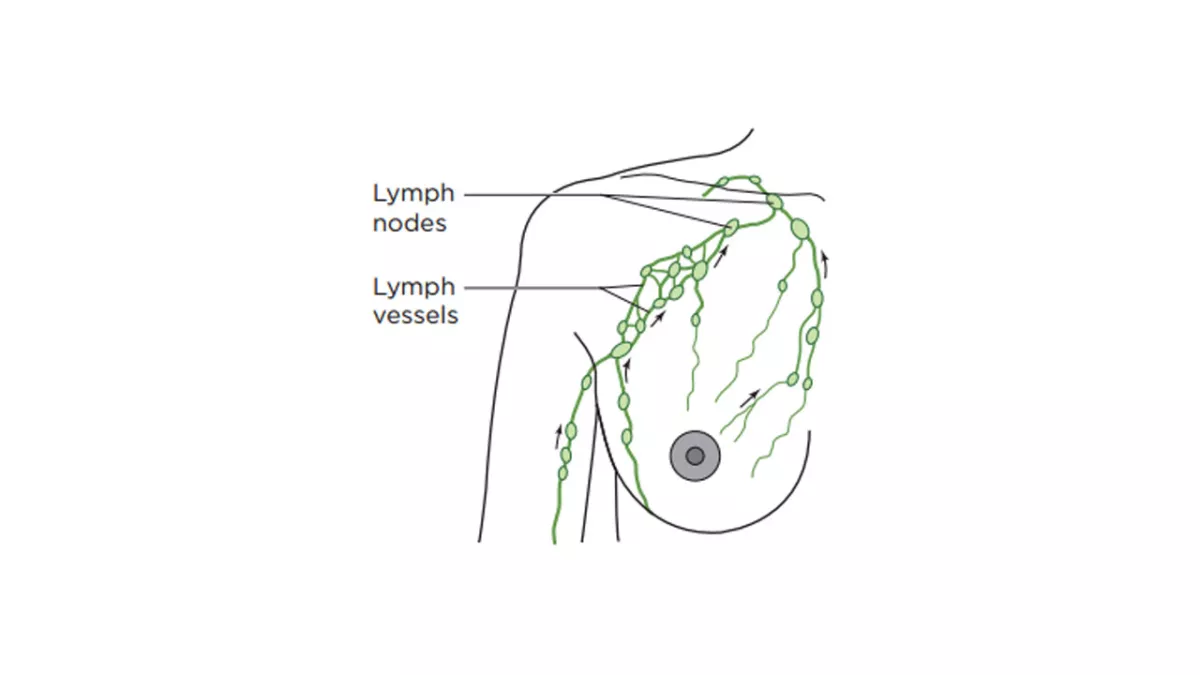
\includegraphics[width=\textwidth]{../figs/introduction/lymphatic_system_in_a_breast.png}
                        \caption{Lymphatic System Overview \cite{RefWorks:RefID:37-memorialsurgery}.}
                        \label{fig:introduction:lymphatic_system_in_a_breast}
                \end{subfigure}
                \begin{subfigure}[b]{0.45\textwidth}
                        \centering
                        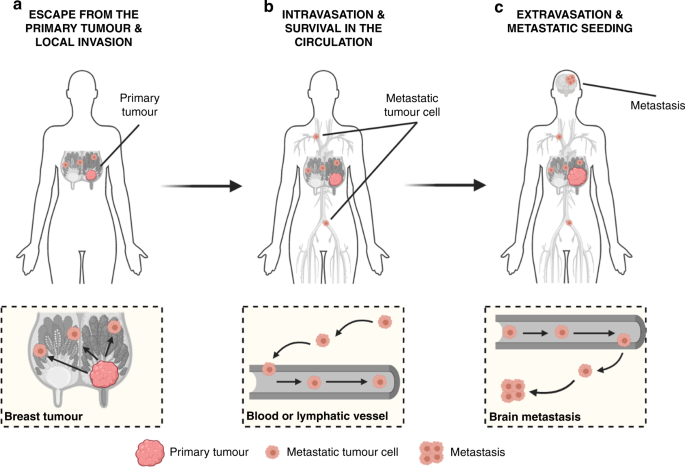
\includegraphics[width=\textwidth]{../figs/introduction/process_of_metastatic_breast_cancer.png}
                        \caption{Lymph Nodes Overview \cite{RefWorks:RefID:364-riggio2020lingering}.}
                        \label{fig:introduction:lymphatic_process_of_metastatic_breast_cancer}
                \end{subfigure}
        \end{minipage}
        \caption{Lymphatic System and Lymph Nodes Overview \cite{RefWorks:RefID:364-riggio2020lingering} \cite{RefWorks:RefID:37-memorialsurgery}.}
        \label{fig:introduction:lymphatic_system_and_nodes_overview}
\end{figure}

\subsection{Treatment of Breast Cancer\label{sec:introduction:treatmentofbreastcancer}}

\subsubsection{Stages of Breast Cancer\label{sec:introduction:breastcancer:stagesofbreastcancer}}
% Early vs late stage
Breast cancer is classified in stages ranging from 0 to IV based on the cancer's characteristics such as tumor size~\cite{RefWorks:RefID:151-2025breast}.

Stage 0 breast cancer is described as non-invasive, meaning the cancer cells are confined to the ducts or lobules in the breast and have not spread to surrounding healthy tissue~\cite{RefWorks:RefID:151-2025breast}.

Stage I breast cancer is invasive, meaning the cancer cells have spread to surrounding healthy tissue. In stage I breast cancer, the tumor is up to 2cm in size but invading cancer cells are no more than 1mm. Stage I is classified as either IA or IB depending on the sevarity of the cancer.~\cite{RefWorks:RefID:151-2025breast}.

Stage II breast cancer is used when the cancer is larger than 2cm but no larger than 5cm, or if the cancer has spread to one to three nearby lymph nodes. Similar to stage I breast cancer, stage II breast cancer can be subdivided into IIA and IIB~\cite{RefWorks:RefID:151-2025breast}.

Stage II breast cancer can be divided into IIIA, IIIB, and IIIC. This stage describes invasive breast cancer that is larger than 5cm or is found in four to nine nearby lymph nodes (IIIA), has spread to the chest wall or skin of the breast (IIIB), or has spread to ten or more nearby lymph nodes or to lymph nodes above or below the collarbone (IIIC)~\cite{RefWorks:RefID:151-2025breast}.

Lastly, stage IV breast cancer describes cancer that has metastasized, or spread, to other parts of the body such as the lungs, liver, bones, or brain~\cite{RefWorks:RefID:151-2025breast}.

Breast cancer stages can be divided into early and late stage breast cancer. Early-stage breast cancer incudes stages 0, I, and IIA while late-stage breast cancer includes stages IIB, III, and IV~\cite{RefWorks:RefID:365-stages}. Table~\ref{tab:introduction:breastcancer:stages} summarizes the stages of breast cancer. An overview of breast cancer treatment options for early and late stage breast cancer is shown in Figure~\ref{fig:introduction:breast_cancer_treatment_options_overview}.


\begin{table}[h!]
        \centering
        \caption{Stages of Breast Cancer~\cite{RefWorks:RefID:151-2025breast, RefWorks:RefID:365-stages}.}
        \label{tab:introduction:breastcancer:stages}
        \begin{tabular}{|c|c|c|}
                \hline
                \textbf{Stage} & \textbf{Description}                                       & \textbf{Early/Late Stage} \\
                \hline
                0              & Non-invasive, confined to ducts or lobules                 & Early                     \\
                \hline
                I              & Invasive, tumor up to 2cm, invading cells no more than 1mm & Early                     \\
                \hline
                IIA            & Tumor 2-5cm or spread to 1-3 lymph nodes                   & Early                     \\
                \hline
                IIB            & Tumor larger than 5cm or spread to 1-3 lymph nodes         & Late                      \\
                \hline
                IIIA           & Tumor larger than 5cm or found in 4-9 lymph nodes          & Late                      \\
                \hline
                IIIB           & Spread to chest wall or skin of breast                     & Late                      \\
                \hline
                IIIC           & Spread to 10+ lymph nodes or above/below collarbone        & Late                      \\
                \hline
                IV             & Metastasized to other parts of the body                    & Late                      \\
                \hline
        \end{tabular}
\end{table}

\subsubsection{Current Treatment Options\label{sec:introduction:breastcancer:currenttreatmentoptions}}

\subsubsection*{Surgical Options\label{sec:introduction:breastcancer:currenttreatmentoptions:surgicaloptions}}

Treatment options for breast cancer largely depend on the type and stage of the cancer. Surgical choices include a lumpectomy, which removes the tumor and a small margin of surrounding healthy tissue, or a mastectomy, which removes the entire breast~\cite{RefWorks:RefID:165-czajka2023breast}.

A lumpectomy is followed by radiation therapy to kill any stray cancer cells that may remain in the breast. This combination helps lower the risk of recurrence, or the return of the cancer~\cite{RefWorks:RefID:159-depolo2024radiation}. Radiation therapy is performed using high-energy X-rays to damage a cancer cell's DNA, preventing it from dividing further until it dies. Healthy tissue cells grow and divide slower than cancer cells, allowing them to repair themselves after radiation therapy while cancer cells cannot~\cite{RefWorks:RefID:159-depolo2024radiation}. See Section~\ref{sec:introduction:radiationtherapy} for more information on radiation therapy.

\subsubsection*{Lymph Node Biopsy\label{sec:introduction:breastcancer:currenttreatmentoptions:lymphnodebiopsy}}
In most surgical treatments for breast cancer, a lymph node biopsy is performed to check if cancer has spread past the breast tissue and to the lymph nodes. Samples from one or more lymph nodes are removed and examined under a microscope for cancer cells~\cite{RefWorks:RefID:37-memorialsurgery}. Standard practice was removing most of the lymph nodes in the underarm, called an axillary dissection. Today, a sentinel lymph node biopsy is more commonly performed to allow a faster recovery time~\cite{RefWorks:RefID:37-memorialsurgery}.

\subsubsection*{Sentinel Lymph Node Biopsy\label{sec:introduction:breastcancer:currenttreatmentoptions:sentinellymphnodebiopsy}}
The sentinel lymph node is the first lymph node that breast cancer cells spread to after leaving the breast. In a sentinel lymph node biopsy, a radioactive tracer (often technetium-99m) and/or a blue dye is injected into the side of the tumor. The tracer(s) travel through the lymphatic system to the sentinel lymph node. The blue stain and radiotracer signal, found with a gamma probe, can be used to identify and excise this lymph node for examination under a microscope for cancer cells~\cite{RefWorks:RefID:37-memorialsurgery},~\cite{RefWorks:RefID:165-czajka2023breast}.

\subsubsection*{Systemic Therapies\label{sec:introduction:breastcancer:currenttreatmentoptions:systemictherapies}}
While breast cancer treatment commonly starts with surgery, systemic therapies such as chemotherapy, hormone therapy, or targeted therapies may also be used~\cite{RefWorks:RefID:37-memorialsurgery}.

Chemotherapy, often called "chemo," uses strong medicines to slow or stop cancer cells from growing further. As chemotherapy often works by attacking cells that divide quickly, it can attack cancer cells but also other healthy cells that divide quickly such as those that make your hair grow. This can lead to side effects such as hair loss and nausea~\cite{RefWorks:RefID:37-memorialsurgery}.

Hormone treatment is used for breast cancer cells that require hormones such as estrogen to grow. This is done by blocking the hormones these cancer cells need to grow. Side effects can include changes in menstrual cycle, hot flashes, and aching bones~\cite{RefWorks:RefID:37-memorialsurgery}.

Targeted therapies, or precision medicines, attack specific characteristics of an individual's cancer cells rather than attacking all rapidly dividing cells like chemotherapy. Targeted therapies can treat the most common breast cancer gene mutations such as BRCA1 and BRCA2, HER2, and PIK3CA. This individualized treatment can lead to less side effects than in chemotherapy~\cite{RefWorks:RefID:37-memorialsurgery}.

\begin{figure}[h!]
        \centering
        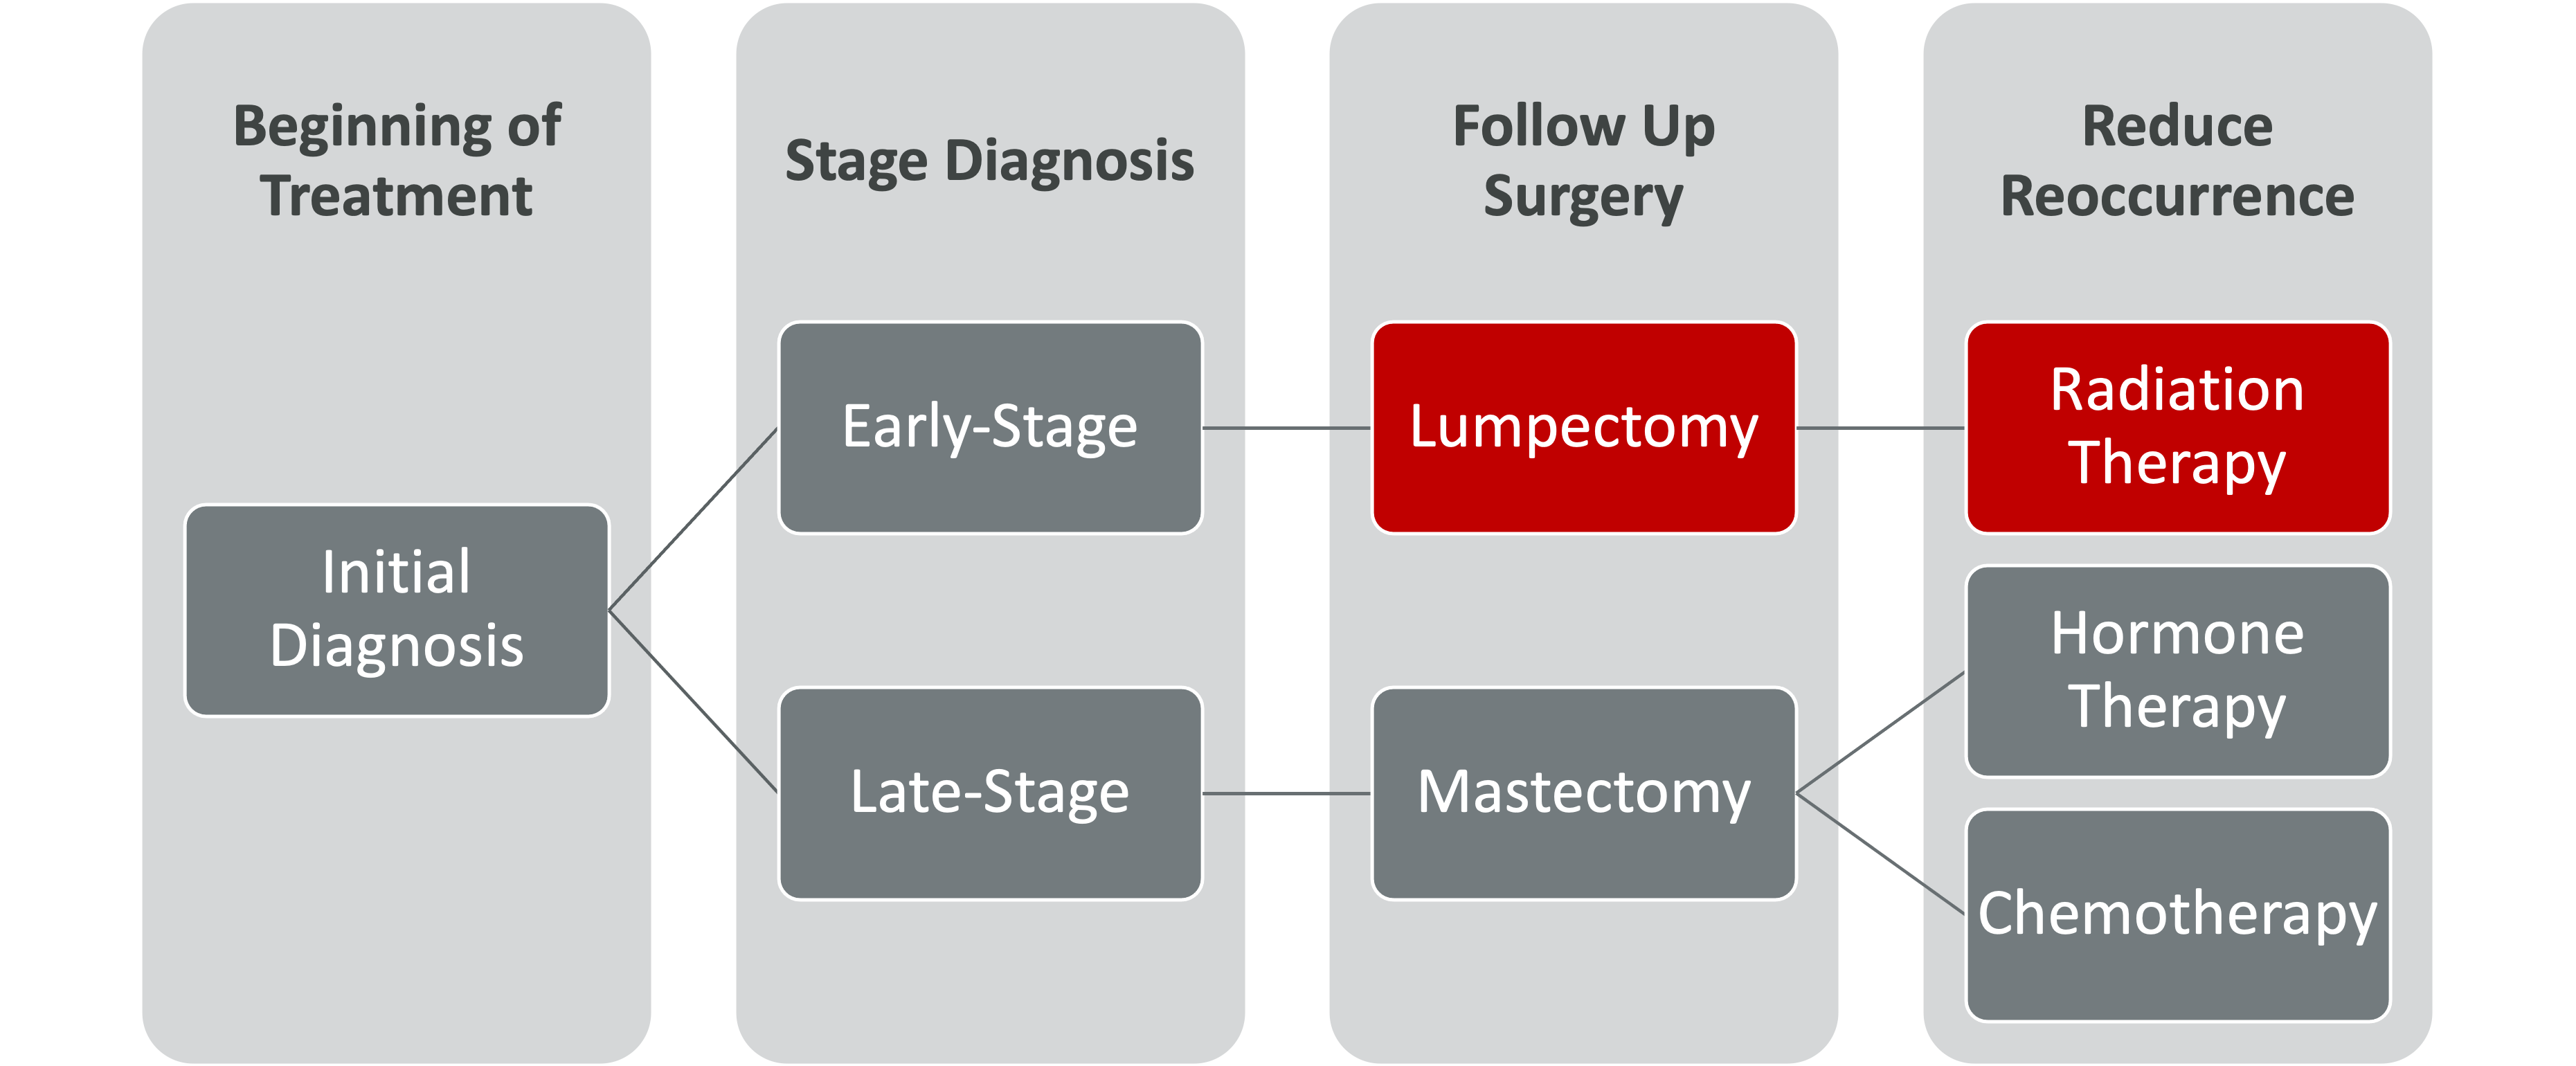
\includegraphics[width=0.6\textwidth]{../figs/introduction/breast_cancer_treatment_process_flowchart.png}
        \caption{Breast Cancer Treatment Options Overview \cite{RefWorks:RefID:37-memorialsurgery}, \cite{RefWorks:RefID:370-einsteinisaac}.}
        \label{fig:introduction:breast_cancer_treatment_options_overview}
\end{figure}

\subsection{Radiation Therapy\label{sec:introduction:radiationtherapy}}
\subsubsection{Radiation Therapy Overview\label{sec:introduction:radiationtherapy:overview}}
As mentioned in Section~\ref{sec:introduction:breastcancer:currenttreatmentoptions:surgicaloptions}, radiation therapy often follows a lumpectomy procedure to kill any stray cancer cells and prevent the cancer from resurfacing. Together, a lumpectomy procedure followed by radiation therapy is commonly known as breast-conserving therapy (BCT). Some compare breast cancer surgery to picking up the large pieces of a broken glass off the floor, while radiation therapy is like vacuuming the remaining shards at the end.

Including radiation therapy after a lumpectomy has been shown to reduce the risk of ipsilateral (same side) recurrence as well as increase overall survival rates~\cite{RefWorks:RefID:157-thomasscience}, ~\cite{RefWorks:RefID:198-jiao2024interobserver}.

\subsubsection{Whole vs Accelerated Partial Breast Irradiation\label{sec:introduction:radiationtherapy:wholevsacceleratedpartialbreastirradiation}}
Patients undergoing BCT can receive either whole breast irradation (WBI) or accelerated partial breast irradiation (APBI). WBI is the more common of the two techniques, although APBI has been gaining traction in recent years due to its unique benefits~\cite{RefWorks:RefID:157-thomasscience}.

WBI is delivered over the course of five to six weeks while APBI is delivered over the course of one week. APBI also limits radiation exposure to 1-2 cm margin of healthy tissue surrounding the tumor site. This limited exposure reduces radiation exposure risks to surrounding organs such as lungs, heart, or ribs. APBI also resulted in higher rates of "excellent/good" cosmetic outcomes compared to WBI (81\% vs 63\% respectively)~\cite{RefWorks:RefID:157-thomasscience}. Comparison of radiation exposure in WBI vs APBI is illustrated in Figure~\ref{fig:introduction:WBI_vs_APBI_irradiation_comparison}.

\begin{figure}[h!]
        \centering
        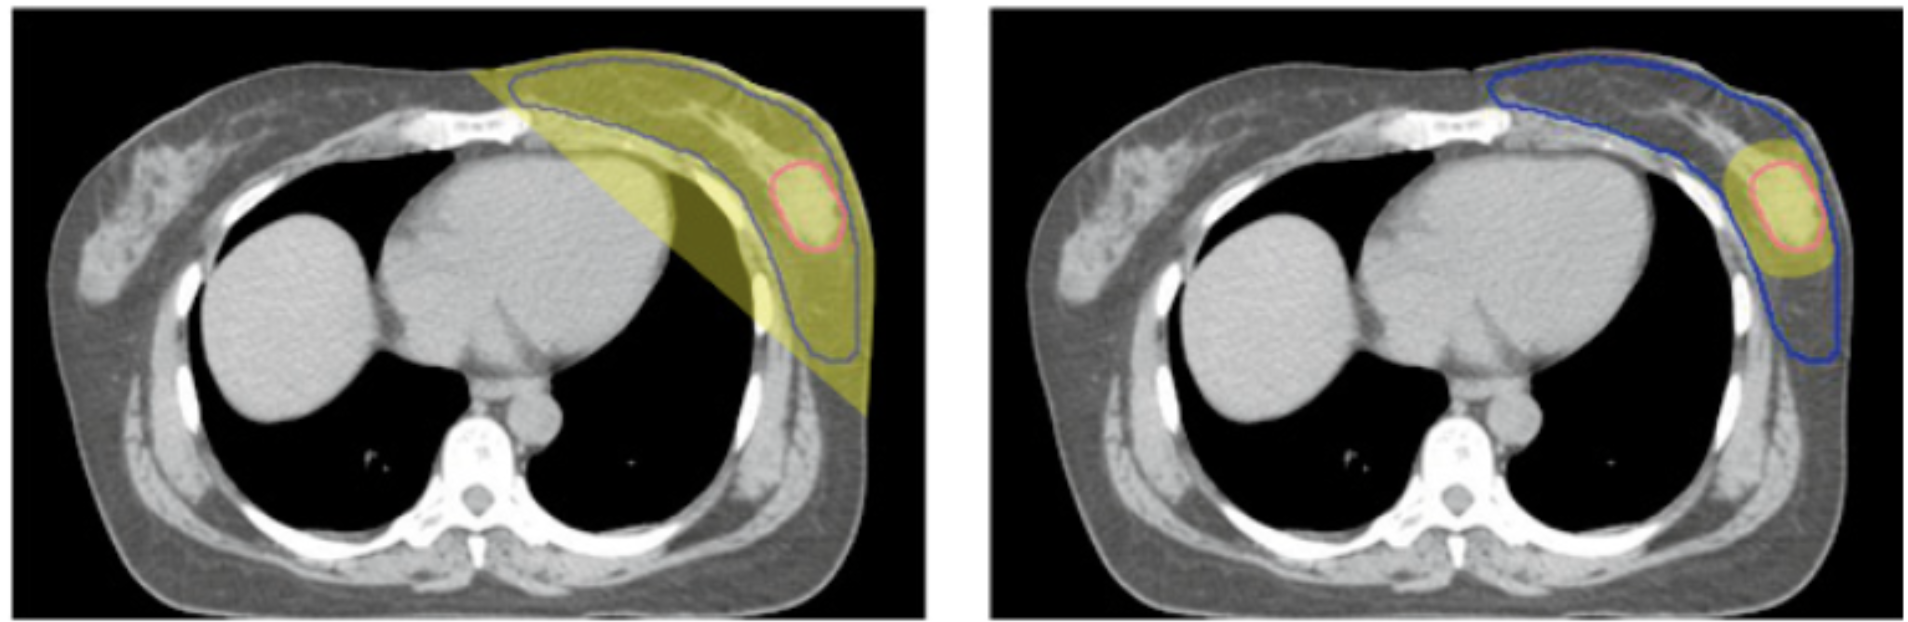
\includegraphics[width=0.6\textwidth]{../figs/introduction/WBI_vs_APBI_irradiation_comparison.png}
        \caption{Comparison of radiation exposure between Whole Breast Irradiation (WBI) (left) and Accelerated Partial Breast Irradiation (APBI) (right) \cite{RefWorks:RefID:157-thomasscience}. The yellow area indicates the irradiated region.}
        \label{fig:introduction:WBI_vs_APBI_irradiation_comparison}
\end{figure}

\subsubsection{Radiation Therapy Treatment Planning\label{sec:introduction:radiationtherapy:treatmentplanning}}
Radiation therapy (WBI or APBI) requires tumor bed delineation to identify and outline the tumor as well as a surrounding healthy tissue margin. This treatment planning ensures radiation is delivered accurately to the tumor site while minimizing exposure to healthy surrounding tissue and organs~\cite{RefWorks:RefID:197-den2015postlumpectomy}.

One concern with tumor bed (TB) delineation is the interobserver variability in accurately marking the TB~\cite{RefWorks:RefID:197-den2015postlumpectomy},~\cite{RefWorks:RefID:179-yang2013tumor}. There are many methods and devices used to assist in TB delineation to address these concerns such as surgical clips, pre-operative imaging, seroma formation, fiducial markers, and other implantable devices~\cite{RefWorks:RefID:179-yang2013tumor},~\cite{RefWorks:RefID:25-acree2022review}.

\subsection{Motivation\label{sec:introduction:motivation}}
The motivation for this work stems from the need to standardize and improve the accuracy and consistency of tumor bed (TB) delineation in radiation therapy following a lumpectomy procedure.

The challenges with accurate TB delineation following a lumpectomy procedure arise because the cancerous tissue has been removed, leaving behind a tumor cavity that is difficult to accurately trace~\cite{RefWorks:RefID:25-acree2022review}. Additionally, unlike other parts of the body, the breast lacks anatomic landmarks to assist with tumor bed delineation~\cite{RefWorks:RefID:344-mitchell2019adaptable}. This need for a marking method is visualized below in Figure~\ref{fig:introduction:need_for_tumor_bed_marker}.

\begin{figure}[h!]
        \centering
        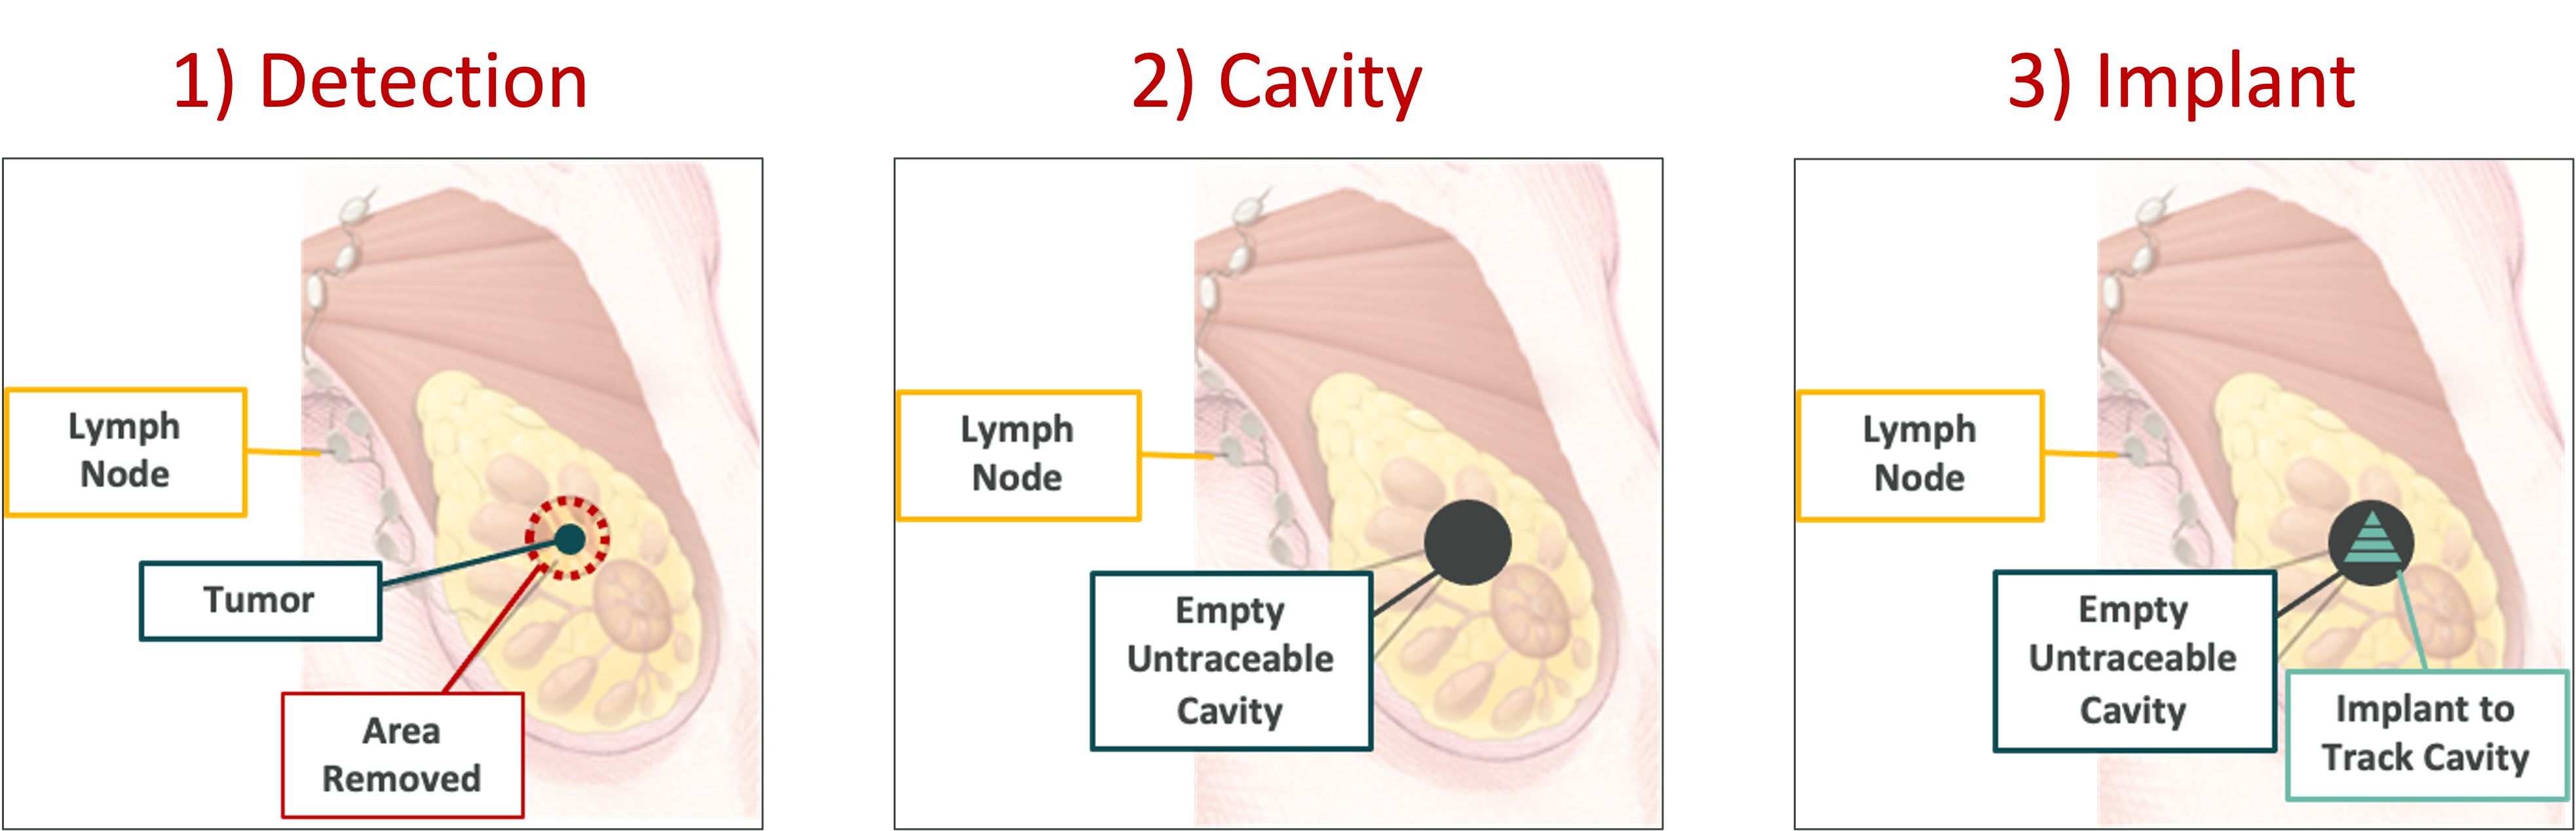
\includegraphics[width=0.6\textwidth]{../figs/introduction/need_for_tumor_bed_marker.png}
        \caption{Motivation for tumor cavity marker following lumpectomy procedure. Adapted from \cite{RefWorks:RefID:38-johnbreastconserving}.}
        \label{fig:introduction:need_for_tumor_bed_marker}
\end{figure}

Current devices and methods used for TB delineation have limitations that affect the overall consistency and accuracy of post-lumpectomy radiation therapy. As over 70\% of breast cancer recurrences occur at the original tumor site, accurate TB delineation and radiation delivery is important in improving patient outcomes~\cite{RefWorks:RefID:25-acree2022review}.

\subsubsection{Importance of Accurate Tumor Bed Delineation\label{sec:introduction:motivation:importanceofaccuratetumorbeddelineation}}
\hl{See if this could use more detail.\\}
Accurate TB delineation is crucial in effective radiation therapy following a lumpectomy procedure given the increasing use of APBI. Since APBI targets a small area of tissue surrounding the tumor bed, accurate delineation is necessary to ensure the radiation dose is delivered precisely to the intended area while minimizing exposure to surrounding healthy tissue and organs~\cite{RefWorks:RefID:197-den2015postlumpectomy}, ~\cite{RefWorks:RefID:25-acree2022review}.

Overestimating TB volume, common in seroma-based delineation, is associated with an increased risk of subcutaneous fibrosis and poorer cosmetic results~\cite{RefWorks:RefID:197-den2015postlumpectomy}. Conversely, underestimating TB volume can lead to insufficient radiation coverage of the tumor bed, increasing the risk of local recurrence~\cite{RefWorks:RefID:198-jiao2024interobserver}. An inaccurate TB volume can
also lead to alteration of management of a radiation boost and completely missing one or more margins of the TB~\cite{RefWorks:RefID:344-mitchell2019adaptable}.

\subsubsection{Current Devices and Methods\label{sec:introduction:motivation:currentdevicesandmethods}}
\hl{See if this could use more detail.\\}
Current devices and methods used for TB delineation include titanium, gold, or liquid fiducial markers/surgical clips, surgeon discretion, seroma formation, or implantable devices~\cite{RefWorks:RefID:25-acree2022review}.

Fiducial markers are solid metal clips inserted around the border of a tumor cavity immediately following the tumor removal~\cite{RefWorks:RefID:358-defining}. These provide a 2D point mapping of the tumor space as shown below in Figure~\ref{fig:introduction:imaging_of_fiducal_clips_in_phantom_breast}.

Liquid fiducial markers were first used as spacers for prostate cancer treatment planning. They have since been repurposed to be used for TB delineation. These markers provide a clearer delineation than solid clips as they conform to the tumor cavity shape~\cite{RefWorks:RefID:25-acree2022review}.

\begin{figure}[h!]
        \centering
        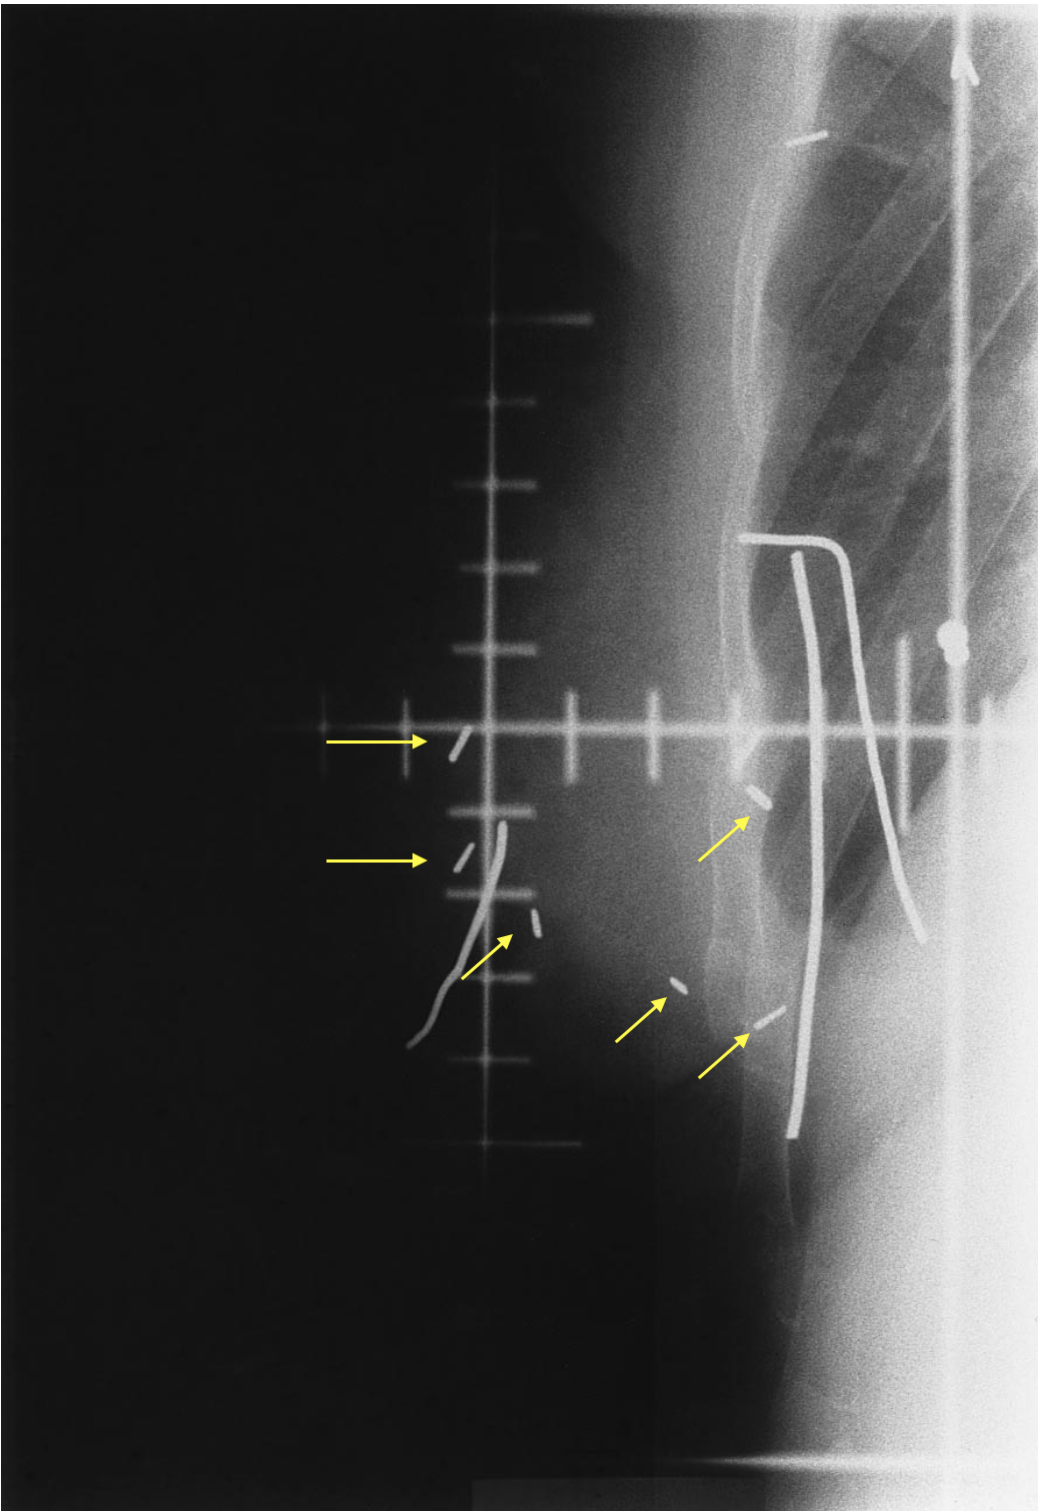
\includegraphics[width=0.6\textwidth]{../figs/introduction/imaging_of_fiducal_clips_in_phantom_breast.png}
        \caption{Imaging of Fiducial Clips in Phantom Breast. Yellow arrows indicate fiducial clips placed around tumor cavity. Adapted from \cite{RefWorks:RefID:178-krawczyk1994importance}.}
        \label{fig:introduction:imaging_of_fiducal_clips_in_phantom_breast}
\end{figure}

Using seroma formation to mark the tumor bed for radiation therapy involves outlining the seroma that forms following a lumpectomy procedure~\cite{RefWorks:RefID:25-acree2022review}.

Lastly, implantable devices can be used to mark the tumor bed. One example is BioZorb (Hologic) which is a 3-dimensional coil-like structure with titanium clips embedded. This device is implanted into the tumor cavity following a lumpectomy procedure and improves on titanium clips alone by creating a 3D outline of the tumor bed. BioZorb was also designed to be reabsorbed into the body within a year~\cite{RefWorks:RefID:25-acree2022review}. BioZorb is shown below in Figure~\ref{fig:introduction:biozorb_implant}.

\begin{figure}[h!]
        \begin{minipage}{0.92\textwidth}
                \centering
                \begin{subfigure}[b]{0.9\textwidth}
                        \centering
                        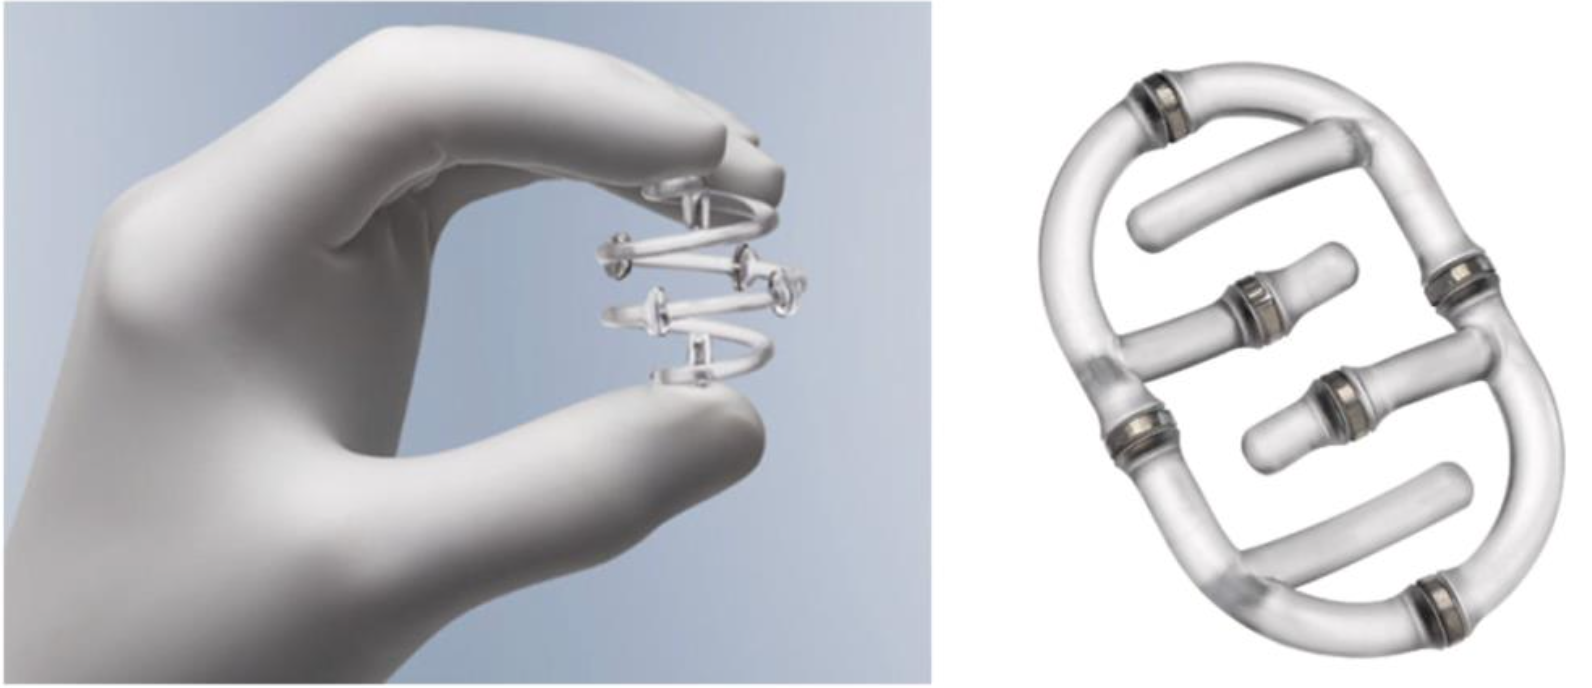
\includegraphics[width=\textwidth]{../figs/introduction/BioZorb_physically.png}
                        \caption{BioZorb physically (top).}
                        \label{fig:introduction:biozorb_physically}
                \end{subfigure}

                \vspace{1em} % optional space between images

                \begin{subfigure}[b]{0.9\textwidth}
                        \centering
                        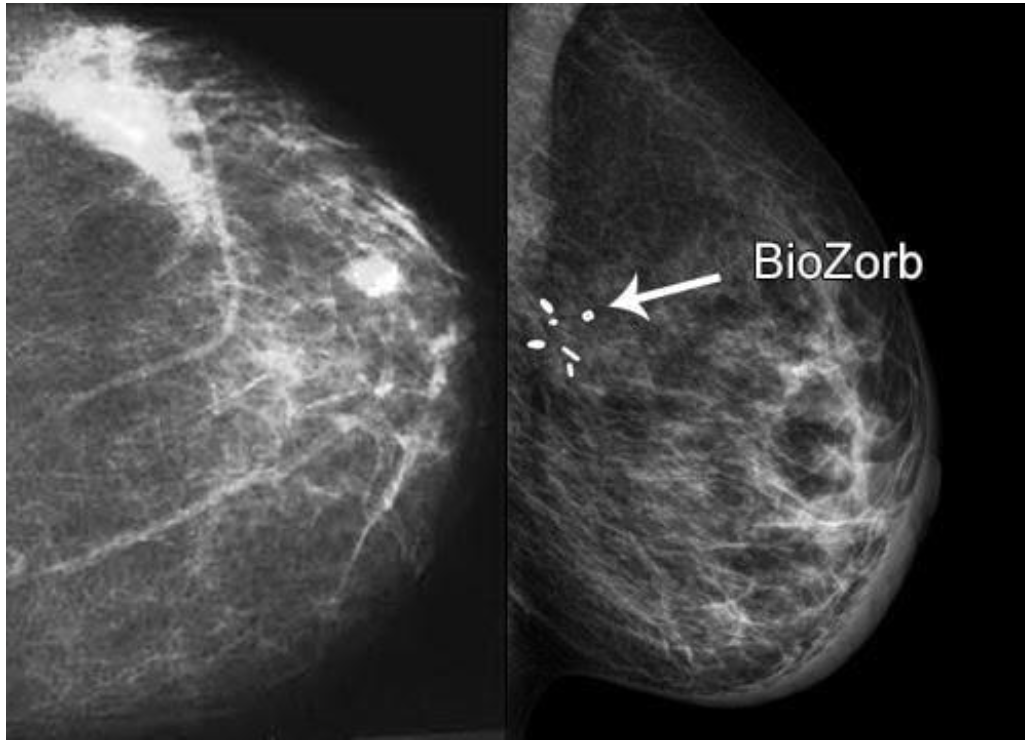
\includegraphics[width=\textwidth]{../figs/introduction/BioZorb_in_imaging.png}
                        \caption{BioZorb in imaging.}
                        \label{fig:introduction:biozorb_in_imaging}
                \end{subfigure}
        \end{minipage}
        \caption{BioZorb, an implantable device to assist with TB delineation~\cite{RefWorks:RefID:370-einsteinisaac}.}
        \label{fig:introduction:biozorb_implant}
\end{figure}

A newer implantable device is Veraform, a continuously radiographically opaque filament that is stitched around the tumor cavity. By being malleable and sewn in place, this device addresses space limitations and migration issues present in other devices~\cite{RefWorks:RefID:344-mitchell2019adaptable}. A simulation showing Veraform in use is shown below in Figure~\ref{fig:introduction:veraform_implant}.
\begin{figure}[h!]
        \centering
        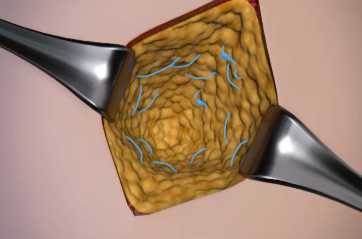
\includegraphics[width=0.6\textwidth]{../figs/introduction/veraform_implant.png}
        \caption{Veraform, an implantable device to assist with TB delineation~\cite{RefWorks:RefID:344-mitchell2019adaptable}.}
        \label{fig:introduction:veraform_implant}
\end{figure}

\subsubsection{Challenges with Current Devices and Methods\label{sec:introduction:motivation:challengeswithcurrentdevicesandmethods}}
\hl{See if this could use more detail.\\}

\subsubsection*{Challenges with Fiducial Markers\label{sec:introduction:motivation:challengeswithcurrentdevicesandmethods:challengeswithfiducialmarkers}}
There are many challenges and inaccuracies that can result from using fiducial markers or surgical clips to create a TB volume. They provide single points of reference which can lead to inaccurate boundaries being drawn, there is no standardized recommendation of how many clips should be used, and clips can migrate over time leading to inaccurate TB localization~\cite{RefWorks:RefID:344-mitchell2019adaptable}. Migration is especially common when patients undergo oncoplastic reconstruction surgery following the lumpectomy procedure. In 2022, it was found the 30,000 breast-conserving therapy patients annually undergo oncoplastic reconstruction surgery~\cite{RefWorks:RefID:25-acree2022review}.

Another concern of surgical clips or fiducial markers is if a re-excision is required. This is when a margin of tissue removed during the lumpectomy is found to contain cancerous cells. When this is the case, a large enough margin surrounding the tumor was not removed, and a re-excision has to be made to remove additional margins. When markers are placed initially, these re-excisions can impact the accuracy of the initial marker placement. It was found that 10\% to 20\% of patients undergoing breast-conserving surgery require a re-excision~\cite{RefWorks:RefID:25-acree2022review}.

\subsubsection*{Challenges with Seroma Formation\label{sec:introduction:motivation:challengeswithcurrentdevicesandmethods:challengeswithseromaformation}}
\hl{Show change in seroma over time visual.\\}

Utilizing seroma formation can be unreliable, as the seroma may not always be localized to the tumor bed, relies on the excision closure method, and time elapsed after surgery\cite{RefWorks:RefID:25-acree2022review}. A seroma may represent the tumor bed, part of the tumor bed, or the entire area in which surgery was performed~\cite{RefWorks:RefID:344-mitchell2019adaptable}.

\subsubsection*{Challenges with Biozorb}
Biozorb was found to provide limited value to patients relative to its high cost~\cite{RefWorks:RefID:344-mitchell2019adaptable}. Additionally, Biozorb was also recalled due to patient discomfort, seroma formation, device migration, and failures to resorb into the body in the designated timeframe~\cite{RefWorks:RefID:296-2024hologic},~\cite{RefWorks:RefID:28-nudelunited}.

\subsubsection{Proposed Solution\label{sec:introduction:motivation:proposedsolution}}
% Explain our research and the proposed mesh
   % describe the problem statement

    \newpage

    \chapter{Contribution 1\label{chap:contrib1}}

\lipsum{}

%%% Local Variables:
%%% mode: latex
%%% TeX-master: "../dissertation"
%%% End:


\newpage
\section{Background\label{introduction:background}}

\subsection{Breast Cancer Overview\label{sec:introduction:breastcanceroverview}}
Breast cancer is a type of cancer that starts in one or both breasts. The left and right breast are each mainly glands, ducts, and fatty tissue. Breast cancer can start in these different parts of the breast or others~\cite{RefWorks:RefID:36-american2021breast}.

\subsubsection{Statistics\label{sec:introduction:breastcancer:statistics}}
Breast cancer accounts for about 30\% of all new cancer cases in U.S. women each year~\cite{RefWorks:RefID:150-2025breast}. The average risk of a woman in the U.S. developing breast cancer sometime in her life is about 1 in 8 (about 13\%)~\cite{RefWorks:RefID:36-american2021breast}. Breast cancer is also the second leading cause of cancer death in women behind lung cancer~\cite{RefWorks:RefID:36-american2021breast}.

\subsubsection{Development and Spread\label{sec:introduction:breastcancer:developmentandspread}}
Breast cancer can start in different parts of the breast, such as the ducts, lobules, or the tissue in between. The cancer can spread when cancer cells are carried to other parts of the body through blood or the lymphatic system. The lymphatic system is a network of small bean-sized glands called lymph nodes, ducts, and vessels that carry clear lymph fluid throughout the body. This clear lymph fluid contains immune system cells to fight infection as well as waste and tissue by-products. This system carries lymph fluid away from the breast; cancer cells can enter the lymph vessels, grow inside lymph nodes, and spread to other parts of the body~\cite{RefWorks:RefID:36-american2021breast}.

The most common areas where lymph vessels of the breast drain into are the underarm (axillary), inside the chest near the breastbone (internal mammary), and around the collar bone (supraclavicular and infraclavicular). Once cancer cells have spread to  the lymph nodes, there is a higher chance of metastases, or spreading, to other parts of the body which is called metastatic breast cancer~\cite{RefWorks:RefID:36-american2021breast}.

The method of cancer cells metastasizing through the lymphatic system is illustrated below in Figure~\ref{fig:introduction:lymphatic_system_in_a_breast} and Figure~\ref{fig:introduction:lymphatic_process_of_metastatic_breast_cancer}.

\begin{figure}[h!]
        \begin{minipage}{0.92\textwidth}
                \centering
                \begin{subfigure}[b]{0.45\textwidth}
                        \centering
                        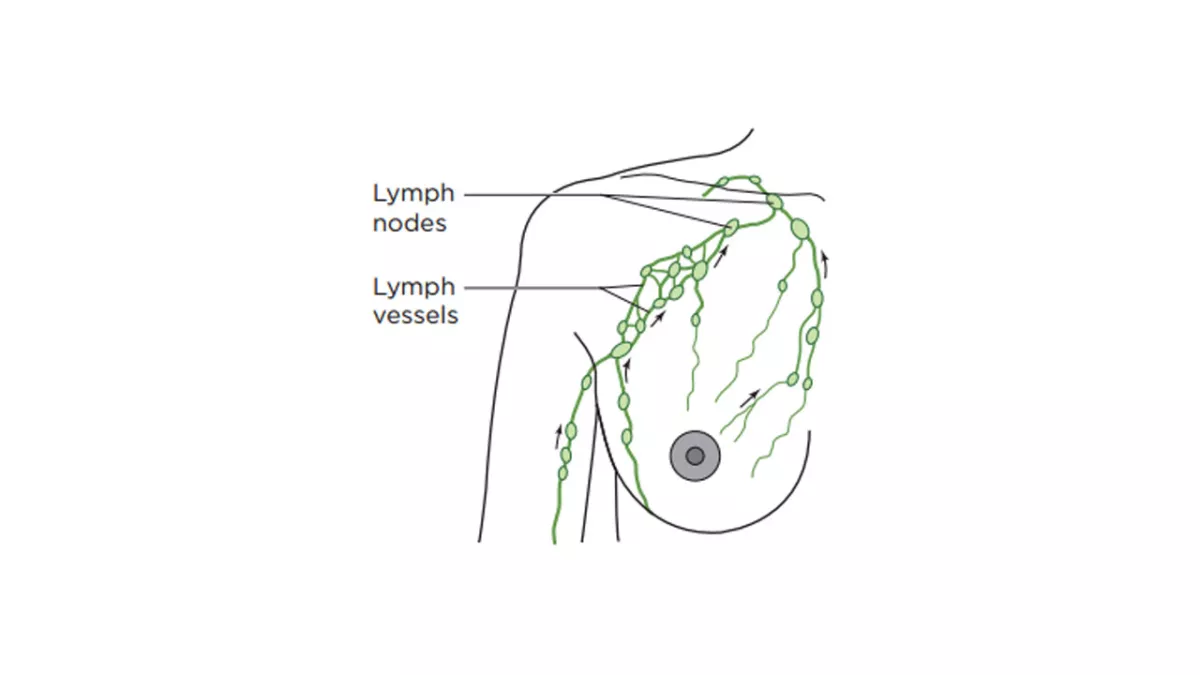
\includegraphics[width=\textwidth]{../figs/introduction/lymphatic_system_in_a_breast.png}
                        \caption{Lymphatic System Overview \cite{RefWorks:RefID:37-memorialsurgery}.}
                        \label{fig:introduction:lymphatic_system_in_a_breast}
                \end{subfigure}
                \begin{subfigure}[b]{0.45\textwidth}
                        \centering
                        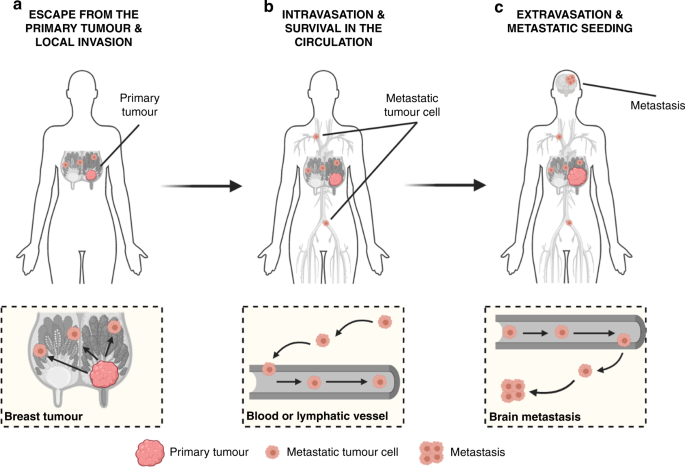
\includegraphics[width=\textwidth]{../figs/introduction/process_of_metastatic_breast_cancer.png}
                        \caption{Lymph Nodes Overview \cite{RefWorks:RefID:364-riggio2020lingering}.}
                        \label{fig:introduction:lymphatic_process_of_metastatic_breast_cancer}
                \end{subfigure}
        \end{minipage}
        \caption{Lymphatic System and Lymph Nodes Overview \cite{RefWorks:RefID:364-riggio2020lingering} \cite{RefWorks:RefID:37-memorialsurgery}.}
        \label{fig:introduction:lymphatic_system_and_nodes_overview}
\end{figure}

\subsection{Treatment of Breast Cancer\label{sec:introduction:treatmentofbreastcancer}}

\subsubsection{Stages of Breast Cancer\label{sec:introduction:breastcancer:stagesofbreastcancer}}
% Early vs late stage
Breast cancer is classified in stages ranging from 0 to IV based on the cancer's characteristics such as tumor size~\cite{RefWorks:RefID:151-2025breast}.

Stage 0 breast cancer is described as non-invasive, meaning the cancer cells are confined to the ducts or lobules in the breast and have not spread to surrounding healthy tissue~\cite{RefWorks:RefID:151-2025breast}.

Stage I breast cancer is invasive, meaning the cancer cells have spread to surrounding healthy tissue. In stage I breast cancer, the tumor is up to 2cm in size but invading cancer cells are no more than 1mm. Stage I is classified as either IA or IB depending on the sevarity of the cancer.~\cite{RefWorks:RefID:151-2025breast}.

Stage II breast cancer is used when the cancer is larger than 2cm but no larger than 5cm, or if the cancer has spread to one to three nearby lymph nodes. Similar to stage I breast cancer, stage II breast cancer can be subdivided into IIA and IIB~\cite{RefWorks:RefID:151-2025breast}.

Stage II breast cancer can be divided into IIIA, IIIB, and IIIC. This stage describes invasive breast cancer that is larger than 5cm or is found in four to nine nearby lymph nodes (IIIA), has spread to the chest wall or skin of the breast (IIIB), or has spread to ten or more nearby lymph nodes or to lymph nodes above or below the collarbone (IIIC)~\cite{RefWorks:RefID:151-2025breast}.

Lastly, stage IV breast cancer describes cancer that has metastasized, or spread, to other parts of the body such as the lungs, liver, bones, or brain~\cite{RefWorks:RefID:151-2025breast}.

Breast cancer stages can be divided into early and late stage breast cancer. Early-stage breast cancer incudes stages 0, I, and IIA while late-stage breast cancer includes stages IIB, III, and IV~\cite{RefWorks:RefID:365-stages}. Table~\ref{tab:introduction:breastcancer:stages} summarizes the stages of breast cancer. An overview of breast cancer treatment options for early and late stage breast cancer is shown in Figure~\ref{fig:introduction:breast_cancer_treatment_options_overview}.


\begin{table}[h!]
        \centering
        \caption{Stages of Breast Cancer~\cite{RefWorks:RefID:151-2025breast, RefWorks:RefID:365-stages}.}
        \label{tab:introduction:breastcancer:stages}
        \begin{tabular}{|c|c|c|}
                \hline
                \textbf{Stage} & \textbf{Description}                                       & \textbf{Early/Late Stage} \\
                \hline
                0              & Non-invasive, confined to ducts or lobules                 & Early                     \\
                \hline
                I              & Invasive, tumor up to 2cm, invading cells no more than 1mm & Early                     \\
                \hline
                IIA            & Tumor 2-5cm or spread to 1-3 lymph nodes                   & Early                     \\
                \hline
                IIB            & Tumor larger than 5cm or spread to 1-3 lymph nodes         & Late                      \\
                \hline
                IIIA           & Tumor larger than 5cm or found in 4-9 lymph nodes          & Late                      \\
                \hline
                IIIB           & Spread to chest wall or skin of breast                     & Late                      \\
                \hline
                IIIC           & Spread to 10+ lymph nodes or above/below collarbone        & Late                      \\
                \hline
                IV             & Metastasized to other parts of the body                    & Late                      \\
                \hline
        \end{tabular}
\end{table}

\subsubsection{Current Treatment Options\label{sec:introduction:breastcancer:currenttreatmentoptions}}

\subsubsection*{Surgical Options\label{sec:introduction:breastcancer:currenttreatmentoptions:surgicaloptions}}

Treatment options for breast cancer largely depend on the type and stage of the cancer. Surgical choices include a lumpectomy, which removes the tumor and a small margin of surrounding healthy tissue, or a mastectomy, which removes the entire breast~\cite{RefWorks:RefID:165-czajka2023breast}.

A lumpectomy is followed by radiation therapy to kill any stray cancer cells that may remain in the breast. This combination helps lower the risk of recurrence, or the return of the cancer~\cite{RefWorks:RefID:159-depolo2024radiation}. Radiation therapy is performed using high-energy X-rays to damage a cancer cell's DNA, preventing it from dividing further until it dies. Healthy tissue cells grow and divide slower than cancer cells, allowing them to repair themselves after radiation therapy while cancer cells cannot~\cite{RefWorks:RefID:159-depolo2024radiation}. See Section~\ref{sec:introduction:radiationtherapy} for more information on radiation therapy.

\subsubsection*{Lymph Node Biopsy\label{sec:introduction:breastcancer:currenttreatmentoptions:lymphnodebiopsy}}
In most surgical treatments for breast cancer, a lymph node biopsy is performed to check if cancer has spread past the breast tissue and to the lymph nodes. Samples from one or more lymph nodes are removed and examined under a microscope for cancer cells~\cite{RefWorks:RefID:37-memorialsurgery}. Standard practice was removing most of the lymph nodes in the underarm, called an axillary dissection. Today, a sentinel lymph node biopsy is more commonly performed to allow a faster recovery time~\cite{RefWorks:RefID:37-memorialsurgery}.

\subsubsection*{Sentinel Lymph Node Biopsy\label{sec:introduction:breastcancer:currenttreatmentoptions:sentinellymphnodebiopsy}}
The sentinel lymph node is the first lymph node that breast cancer cells spread to after leaving the breast. In a sentinel lymph node biopsy, a radioactive tracer (often technetium-99m) and/or a blue dye is injected into the side of the tumor. The tracer(s) travel through the lymphatic system to the sentinel lymph node. The blue stain and radiotracer signal, found with a gamma probe, can be used to identify and excise this lymph node for examination under a microscope for cancer cells~\cite{RefWorks:RefID:37-memorialsurgery},~\cite{RefWorks:RefID:165-czajka2023breast}.

\subsubsection*{Systemic Therapies\label{sec:introduction:breastcancer:currenttreatmentoptions:systemictherapies}}
While breast cancer treatment commonly starts with surgery, systemic therapies such as chemotherapy, hormone therapy, or targeted therapies may also be used~\cite{RefWorks:RefID:37-memorialsurgery}.

Chemotherapy, often called "chemo," uses strong medicines to slow or stop cancer cells from growing further. As chemotherapy often works by attacking cells that divide quickly, it can attack cancer cells but also other healthy cells that divide quickly such as those that make your hair grow. This can lead to side effects such as hair loss and nausea~\cite{RefWorks:RefID:37-memorialsurgery}.

Hormone treatment is used for breast cancer cells that require hormones such as estrogen to grow. This is done by blocking the hormones these cancer cells need to grow. Side effects can include changes in menstrual cycle, hot flashes, and aching bones~\cite{RefWorks:RefID:37-memorialsurgery}.

Targeted therapies, or precision medicines, attack specific characteristics of an individual's cancer cells rather than attacking all rapidly dividing cells like chemotherapy. Targeted therapies can treat the most common breast cancer gene mutations such as BRCA1 and BRCA2, HER2, and PIK3CA. This individualized treatment can lead to less side effects than in chemotherapy~\cite{RefWorks:RefID:37-memorialsurgery}.

\begin{figure}[h!]
        \centering
        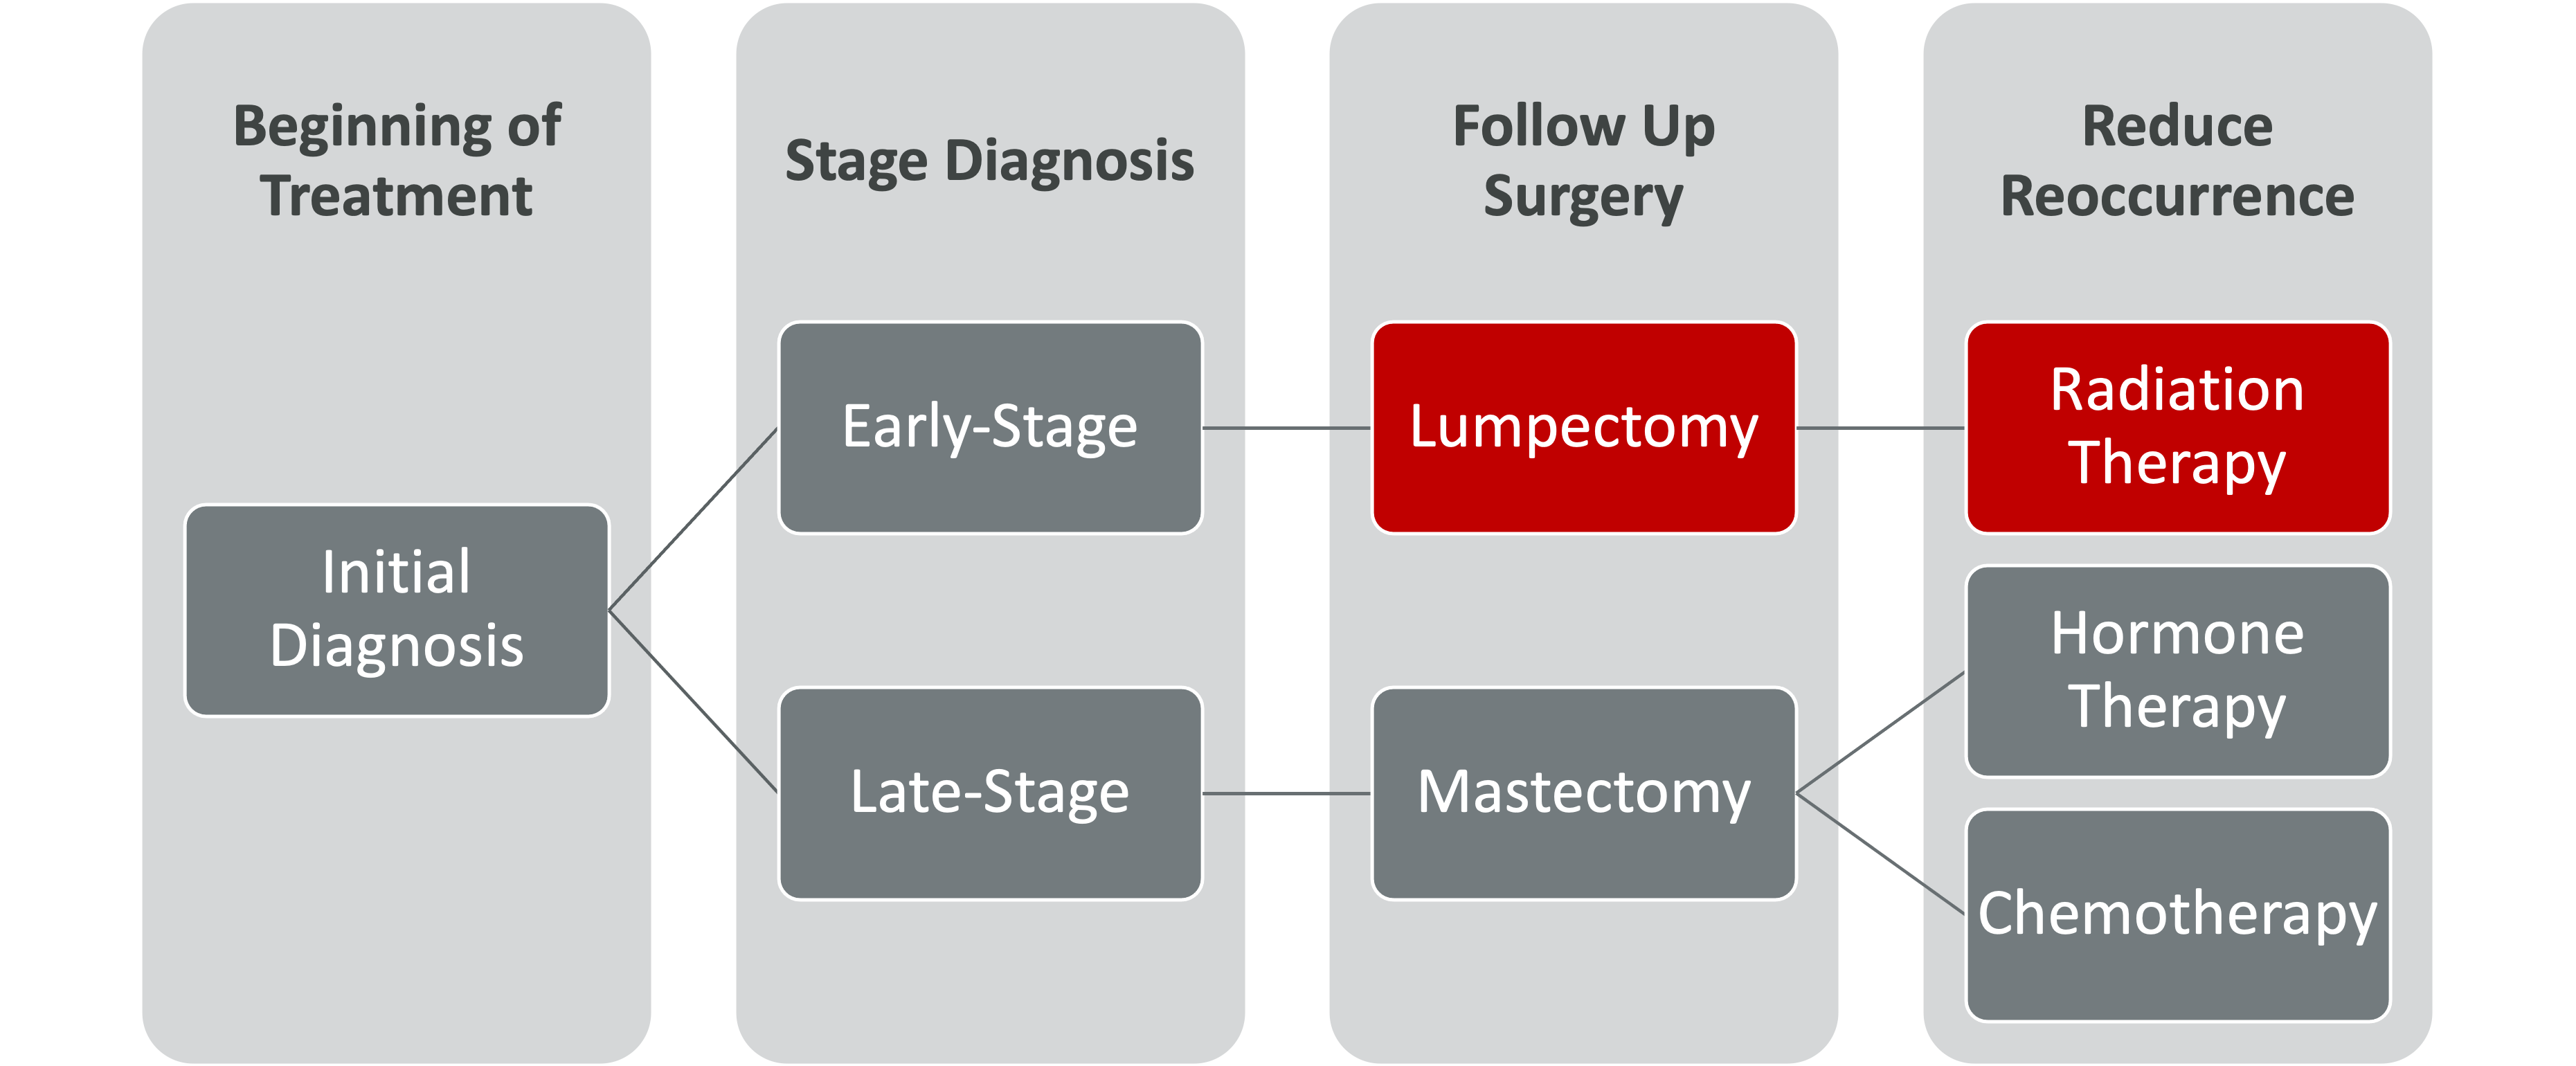
\includegraphics[width=0.6\textwidth]{../figs/introduction/breast_cancer_treatment_process_flowchart.png}
        \caption{Breast Cancer Treatment Options Overview \cite{RefWorks:RefID:37-memorialsurgery}, \cite{RefWorks:RefID:370-einsteinisaac}.}
        \label{fig:introduction:breast_cancer_treatment_options_overview}
\end{figure}

\subsection{Radiation Therapy\label{sec:introduction:radiationtherapy}}
\subsubsection{Radiation Therapy Overview\label{sec:introduction:radiationtherapy:overview}}
As mentioned in Section~\ref{sec:introduction:breastcancer:currenttreatmentoptions:surgicaloptions}, radiation therapy often follows a lumpectomy procedure to kill any stray cancer cells and prevent the cancer from resurfacing. Together, a lumpectomy procedure followed by radiation therapy is commonly known as breast-conserving therapy (BCT). Some compare breast cancer surgery to picking up the large pieces of a broken glass off the floor, while radiation therapy is like vacuuming the remaining shards at the end.

Including radiation therapy after a lumpectomy has been shown to reduce the risk of ipsilateral (same side) recurrence as well as increase overall survival rates~\cite{RefWorks:RefID:157-thomasscience}, ~\cite{RefWorks:RefID:198-jiao2024interobserver}.

\subsubsection{Whole vs Accelerated Partial Breast Irradiation\label{sec:introduction:radiationtherapy:wholevsacceleratedpartialbreastirradiation}}
Patients undergoing BCT can receive either whole breast irradation (WBI) or accelerated partial breast irradiation (APBI). WBI is the more common of the two techniques, although APBI has been gaining traction in recent years due to its unique benefits~\cite{RefWorks:RefID:157-thomasscience}.

WBI is delivered over the course of five to six weeks while APBI is delivered over the course of one week. APBI also limits radiation exposure to 1-2 cm margin of healthy tissue surrounding the tumor site. This limited exposure reduces radiation exposure risks to surrounding organs such as lungs, heart, or ribs. APBI also resulted in higher rates of "excellent/good" cosmetic outcomes compared to WBI (81\% vs 63\% respectively)~\cite{RefWorks:RefID:157-thomasscience}. Comparison of radiation exposure in WBI vs APBI is illustrated in Figure~\ref{fig:introduction:WBI_vs_APBI_irradiation_comparison}.

\begin{figure}[h!]
        \centering
        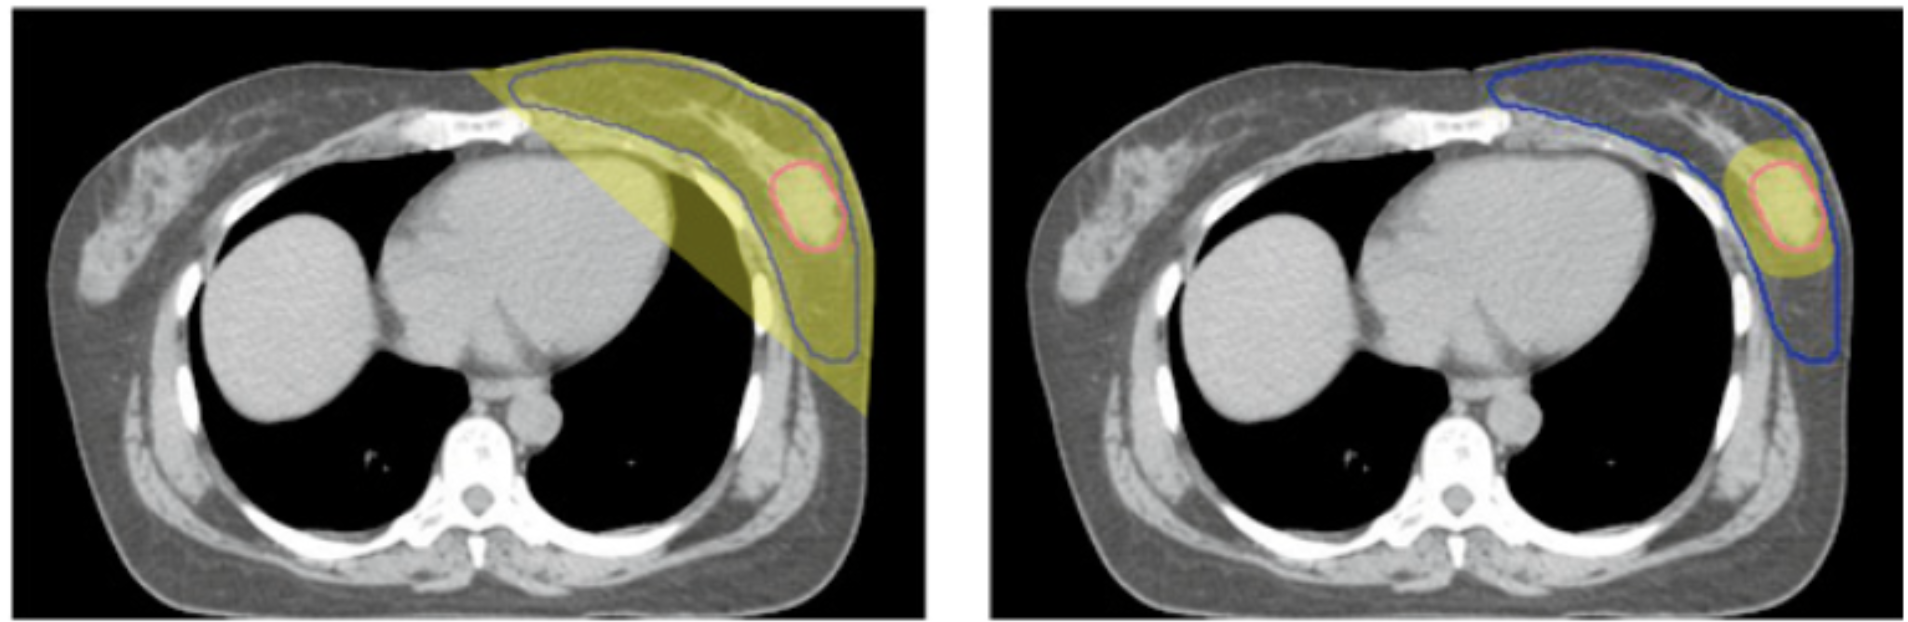
\includegraphics[width=0.6\textwidth]{../figs/introduction/WBI_vs_APBI_irradiation_comparison.png}
        \caption{Comparison of radiation exposure between Whole Breast Irradiation (WBI) (left) and Accelerated Partial Breast Irradiation (APBI) (right) \cite{RefWorks:RefID:157-thomasscience}. The yellow area indicates the irradiated region.}
        \label{fig:introduction:WBI_vs_APBI_irradiation_comparison}
\end{figure}

\subsubsection{Radiation Therapy Treatment Planning\label{sec:introduction:radiationtherapy:treatmentplanning}}
Radiation therapy (WBI or APBI) requires tumor bed delineation to identify and outline the tumor as well as a surrounding healthy tissue margin. This treatment planning ensures radiation is delivered accurately to the tumor site while minimizing exposure to healthy surrounding tissue and organs~\cite{RefWorks:RefID:197-den2015postlumpectomy}.

One concern with tumor bed (TB) delineation is the interobserver variability in accurately marking the TB~\cite{RefWorks:RefID:197-den2015postlumpectomy},~\cite{RefWorks:RefID:179-yang2013tumor}. There are many methods and devices used to assist in TB delineation to address these concerns such as surgical clips, pre-operative imaging, seroma formation, fiducial markers, and other implantable devices~\cite{RefWorks:RefID:179-yang2013tumor},~\cite{RefWorks:RefID:25-acree2022review}.

\subsection{Motivation\label{sec:introduction:motivation}}
The motivation for this work stems from the need to standardize and improve the accuracy and consistency of tumor bed (TB) delineation in radiation therapy following a lumpectomy procedure.

The challenges with accurate TB delineation following a lumpectomy procedure arise because the cancerous tissue has been removed, leaving behind a tumor cavity that is difficult to accurately trace~\cite{RefWorks:RefID:25-acree2022review}. Additionally, unlike other parts of the body, the breast lacks anatomic landmarks to assist with tumor bed delineation~\cite{RefWorks:RefID:344-mitchell2019adaptable}. This need for a marking method is visualized below in Figure~\ref{fig:introduction:need_for_tumor_bed_marker}.

\begin{figure}[h!]
        \centering
        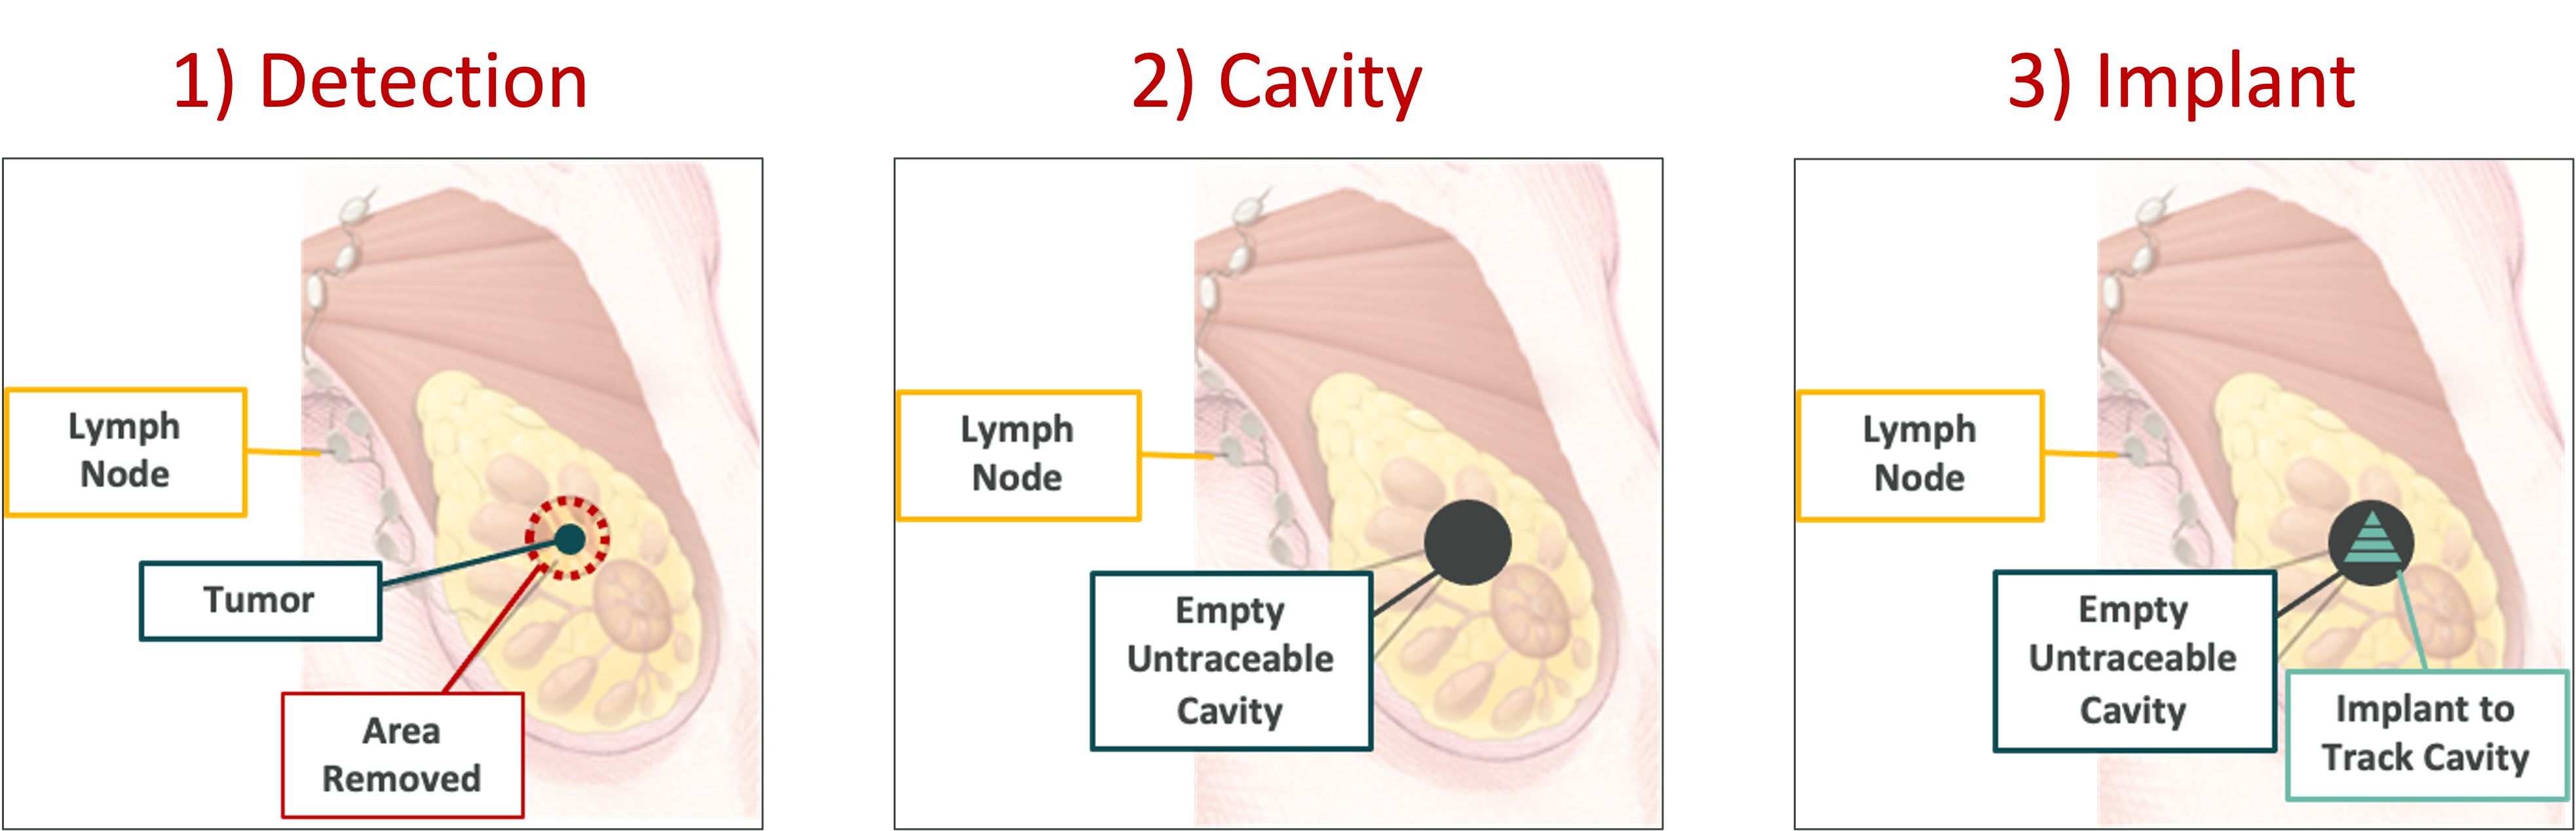
\includegraphics[width=0.6\textwidth]{../figs/introduction/need_for_tumor_bed_marker.png}
        \caption{Motivation for tumor cavity marker following lumpectomy procedure. Adapted from \cite{RefWorks:RefID:38-johnbreastconserving}.}
        \label{fig:introduction:need_for_tumor_bed_marker}
\end{figure}

Current devices and methods used for TB delineation have limitations that affect the overall consistency and accuracy of post-lumpectomy radiation therapy. As over 70\% of breast cancer recurrences occur at the original tumor site, accurate TB delineation and radiation delivery is important in improving patient outcomes~\cite{RefWorks:RefID:25-acree2022review}.

\subsubsection{Importance of Accurate Tumor Bed Delineation\label{sec:introduction:motivation:importanceofaccuratetumorbeddelineation}}
\hl{See if this could use more detail.\\}
Accurate TB delineation is crucial in effective radiation therapy following a lumpectomy procedure given the increasing use of APBI. Since APBI targets a small area of tissue surrounding the tumor bed, accurate delineation is necessary to ensure the radiation dose is delivered precisely to the intended area while minimizing exposure to surrounding healthy tissue and organs~\cite{RefWorks:RefID:197-den2015postlumpectomy}, ~\cite{RefWorks:RefID:25-acree2022review}.

Overestimating TB volume, common in seroma-based delineation, is associated with an increased risk of subcutaneous fibrosis and poorer cosmetic results~\cite{RefWorks:RefID:197-den2015postlumpectomy}. Conversely, underestimating TB volume can lead to insufficient radiation coverage of the tumor bed, increasing the risk of local recurrence~\cite{RefWorks:RefID:198-jiao2024interobserver}. An inaccurate TB volume can
also lead to alteration of management of a radiation boost and completely missing one or more margins of the TB~\cite{RefWorks:RefID:344-mitchell2019adaptable}.

\subsubsection{Current Devices and Methods\label{sec:introduction:motivation:currentdevicesandmethods}}
\hl{See if this could use more detail.\\}
Current devices and methods used for TB delineation include titanium, gold, or liquid fiducial markers/surgical clips, surgeon discretion, seroma formation, or implantable devices~\cite{RefWorks:RefID:25-acree2022review}.

Fiducial markers are solid metal clips inserted around the border of a tumor cavity immediately following the tumor removal~\cite{RefWorks:RefID:358-defining}. These provide a 2D point mapping of the tumor space as shown below in Figure~\ref{fig:introduction:imaging_of_fiducal_clips_in_phantom_breast}.

Liquid fiducial markers were first used as spacers for prostate cancer treatment planning. They have since been repurposed to be used for TB delineation. These markers provide a clearer delineation than solid clips as they conform to the tumor cavity shape~\cite{RefWorks:RefID:25-acree2022review}.

\begin{figure}[h!]
        \centering
        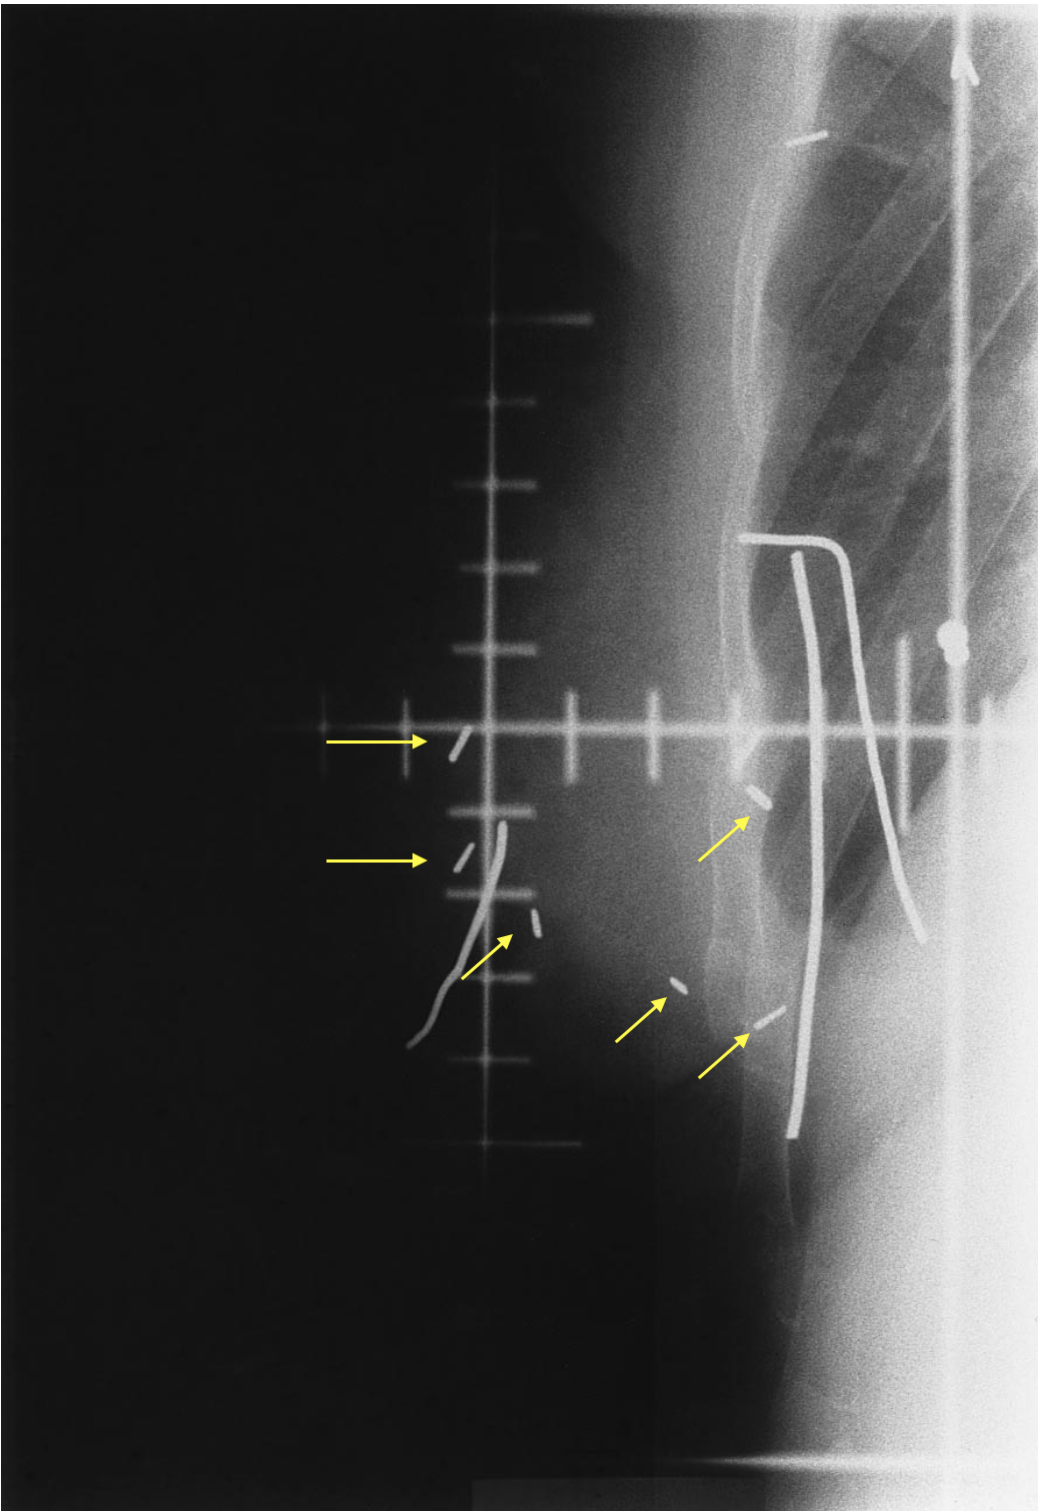
\includegraphics[width=0.6\textwidth]{../figs/introduction/imaging_of_fiducal_clips_in_phantom_breast.png}
        \caption{Imaging of Fiducial Clips in Phantom Breast. Yellow arrows indicate fiducial clips placed around tumor cavity. Adapted from \cite{RefWorks:RefID:178-krawczyk1994importance}.}
        \label{fig:introduction:imaging_of_fiducal_clips_in_phantom_breast}
\end{figure}

Using seroma formation to mark the tumor bed for radiation therapy involves outlining the seroma that forms following a lumpectomy procedure~\cite{RefWorks:RefID:25-acree2022review}.

Lastly, implantable devices can be used to mark the tumor bed. One example is BioZorb (Hologic) which is a 3-dimensional coil-like structure with titanium clips embedded. This device is implanted into the tumor cavity following a lumpectomy procedure and improves on titanium clips alone by creating a 3D outline of the tumor bed. BioZorb was also designed to be reabsorbed into the body within a year~\cite{RefWorks:RefID:25-acree2022review}. BioZorb is shown below in Figure~\ref{fig:introduction:biozorb_implant}.

\begin{figure}[h!]
        \begin{minipage}{0.92\textwidth}
                \centering
                \begin{subfigure}[b]{0.9\textwidth}
                        \centering
                        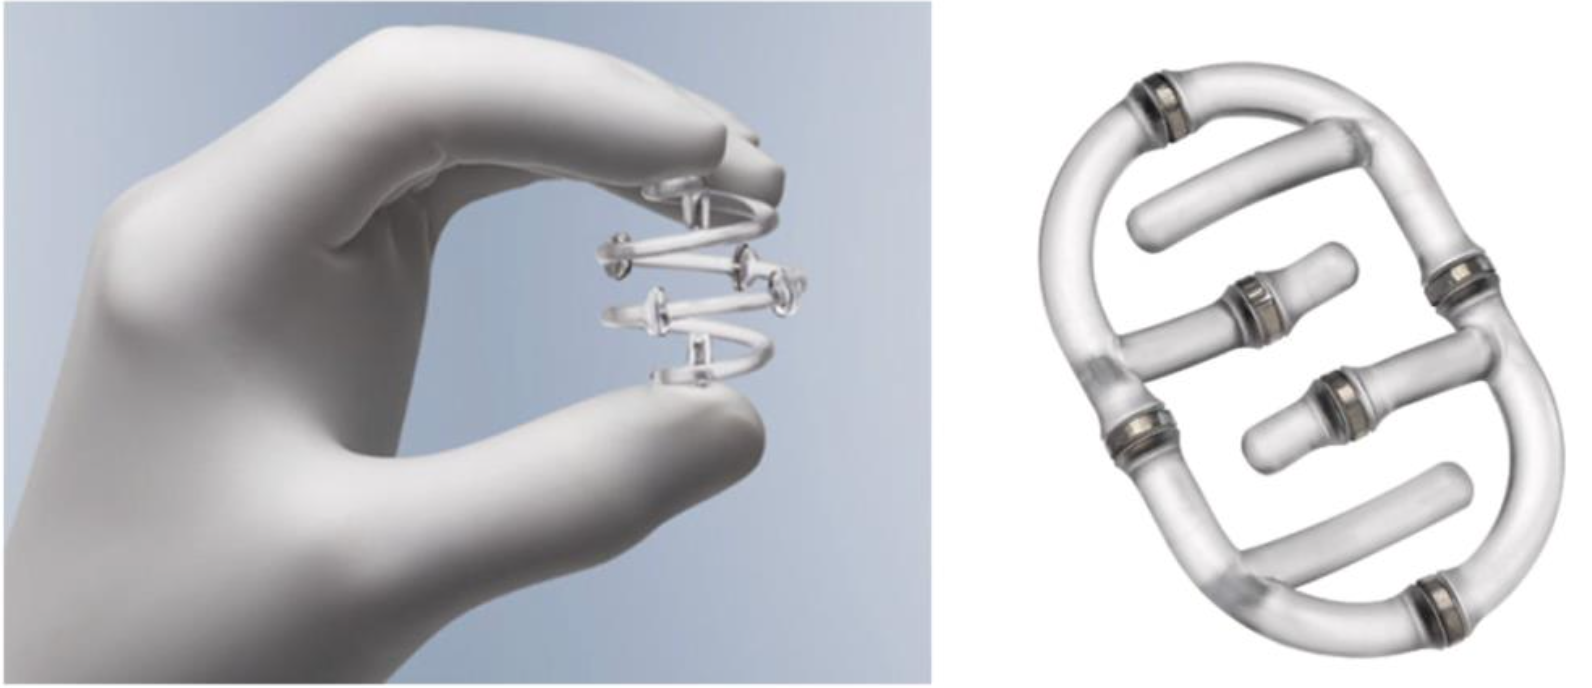
\includegraphics[width=\textwidth]{../figs/introduction/BioZorb_physically.png}
                        \caption{BioZorb physically (top).}
                        \label{fig:introduction:biozorb_physically}
                \end{subfigure}

                \vspace{1em} % optional space between images

                \begin{subfigure}[b]{0.9\textwidth}
                        \centering
                        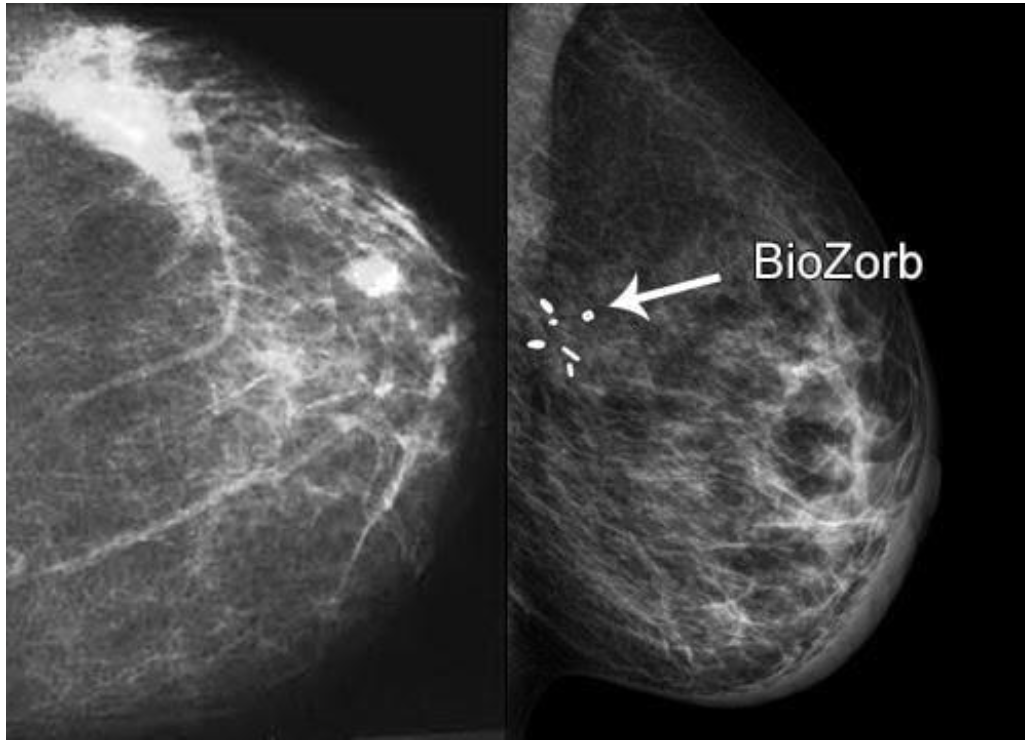
\includegraphics[width=\textwidth]{../figs/introduction/BioZorb_in_imaging.png}
                        \caption{BioZorb in imaging.}
                        \label{fig:introduction:biozorb_in_imaging}
                \end{subfigure}
        \end{minipage}
        \caption{BioZorb, an implantable device to assist with TB delineation~\cite{RefWorks:RefID:370-einsteinisaac}.}
        \label{fig:introduction:biozorb_implant}
\end{figure}

A newer implantable device is Veraform, a continuously radiographically opaque filament that is stitched around the tumor cavity. By being malleable and sewn in place, this device addresses space limitations and migration issues present in other devices~\cite{RefWorks:RefID:344-mitchell2019adaptable}. A simulation showing Veraform in use is shown below in Figure~\ref{fig:introduction:veraform_implant}.
\begin{figure}[h!]
        \centering
        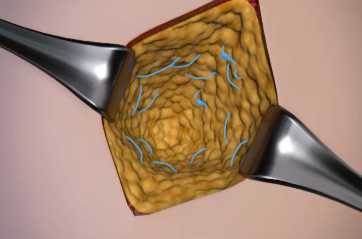
\includegraphics[width=0.6\textwidth]{../figs/introduction/veraform_implant.png}
        \caption{Veraform, an implantable device to assist with TB delineation~\cite{RefWorks:RefID:344-mitchell2019adaptable}.}
        \label{fig:introduction:veraform_implant}
\end{figure}

\subsubsection{Challenges with Current Devices and Methods\label{sec:introduction:motivation:challengeswithcurrentdevicesandmethods}}
\hl{See if this could use more detail.\\}

\subsubsection*{Challenges with Fiducial Markers\label{sec:introduction:motivation:challengeswithcurrentdevicesandmethods:challengeswithfiducialmarkers}}
There are many challenges and inaccuracies that can result from using fiducial markers or surgical clips to create a TB volume. They provide single points of reference which can lead to inaccurate boundaries being drawn, there is no standardized recommendation of how many clips should be used, and clips can migrate over time leading to inaccurate TB localization~\cite{RefWorks:RefID:344-mitchell2019adaptable}. Migration is especially common when patients undergo oncoplastic reconstruction surgery following the lumpectomy procedure. In 2022, it was found the 30,000 breast-conserving therapy patients annually undergo oncoplastic reconstruction surgery~\cite{RefWorks:RefID:25-acree2022review}.

Another concern of surgical clips or fiducial markers is if a re-excision is required. This is when a margin of tissue removed during the lumpectomy is found to contain cancerous cells. When this is the case, a large enough margin surrounding the tumor was not removed, and a re-excision has to be made to remove additional margins. When markers are placed initially, these re-excisions can impact the accuracy of the initial marker placement. It was found that 10\% to 20\% of patients undergoing breast-conserving surgery require a re-excision~\cite{RefWorks:RefID:25-acree2022review}.

\subsubsection*{Challenges with Seroma Formation\label{sec:introduction:motivation:challengeswithcurrentdevicesandmethods:challengeswithseromaformation}}
\hl{Show change in seroma over time visual.\\}

Utilizing seroma formation can be unreliable, as the seroma may not always be localized to the tumor bed, relies on the excision closure method, and time elapsed after surgery\cite{RefWorks:RefID:25-acree2022review}. A seroma may represent the tumor bed, part of the tumor bed, or the entire area in which surgery was performed~\cite{RefWorks:RefID:344-mitchell2019adaptable}.

\subsubsection*{Challenges with Biozorb}
Biozorb was found to provide limited value to patients relative to its high cost~\cite{RefWorks:RefID:344-mitchell2019adaptable}. Additionally, Biozorb was also recalled due to patient discomfort, seroma formation, device migration, and failures to resorb into the body in the designated timeframe~\cite{RefWorks:RefID:296-2024hologic},~\cite{RefWorks:RefID:28-nudelunited}.

\subsubsection{Proposed Solution\label{sec:introduction:motivation:proposedsolution}}
% Explain our research and the proposed mesh


\section{Design\label{chapthree:design}}

\lipsum{}

%%% Local Variables:
%%% mode: latex
%%% TeX-master: "../dissertation"
%%% End:


\section{Implementation\label{chap1:impl}}


%%% Local Variables:
%%% mode: latex
%%% TeX-master: "../dissertation"
%%% End:


\section{Evaluation\label{chap1:eval}}

%%% Local Variables:
%%% mode: latex
%%% TeX-master: "../dissertation"
%%% End:


\chapter{Conclusion\label{chap:conclusion}}

\if@ms
In this chapter, we summarize the status of the work presented in this proposal, and outline future plans~\cite{template}.
\else
In this chapter, we summarize the status of the work presented in this dissertation, and outline future plans~\cite{template}.
\fi

\section{Summary\label{sec:conclusion:summary}}

\lipsum{}

\section{Contributions\label{sec:conclusion:contributions}}

\lipsum{}

    % what is your solution
    \chapter{Contribution 2\label{chap:contrib2}}

\lipsum{}

%%% Local Variables:
%%% mode: latex
%%% TeX-master: "../dissertation"
%%% End:


\newpage
\section{Background\label{introduction:background}}

\subsection{Breast Cancer Overview\label{sec:introduction:breastcanceroverview}}
Breast cancer is a type of cancer that starts in one or both breasts. The left and right breast are each mainly glands, ducts, and fatty tissue. Breast cancer can start in these different parts of the breast or others~\cite{RefWorks:RefID:36-american2021breast}.

\subsubsection{Statistics\label{sec:introduction:breastcancer:statistics}}
Breast cancer accounts for about 30\% of all new cancer cases in U.S. women each year~\cite{RefWorks:RefID:150-2025breast}. The average risk of a woman in the U.S. developing breast cancer sometime in her life is about 1 in 8 (about 13\%)~\cite{RefWorks:RefID:36-american2021breast}. Breast cancer is also the second leading cause of cancer death in women behind lung cancer~\cite{RefWorks:RefID:36-american2021breast}.

\subsubsection{Development and Spread\label{sec:introduction:breastcancer:developmentandspread}}
Breast cancer can start in different parts of the breast, such as the ducts, lobules, or the tissue in between. The cancer can spread when cancer cells are carried to other parts of the body through blood or the lymphatic system. The lymphatic system is a network of small bean-sized glands called lymph nodes, ducts, and vessels that carry clear lymph fluid throughout the body. This clear lymph fluid contains immune system cells to fight infection as well as waste and tissue by-products. This system carries lymph fluid away from the breast; cancer cells can enter the lymph vessels, grow inside lymph nodes, and spread to other parts of the body~\cite{RefWorks:RefID:36-american2021breast}.

The most common areas where lymph vessels of the breast drain into are the underarm (axillary), inside the chest near the breastbone (internal mammary), and around the collar bone (supraclavicular and infraclavicular). Once cancer cells have spread to  the lymph nodes, there is a higher chance of metastases, or spreading, to other parts of the body which is called metastatic breast cancer~\cite{RefWorks:RefID:36-american2021breast}.

The method of cancer cells metastasizing through the lymphatic system is illustrated below in Figure~\ref{fig:introduction:lymphatic_system_in_a_breast} and Figure~\ref{fig:introduction:lymphatic_process_of_metastatic_breast_cancer}.

\begin{figure}[h!]
        \begin{minipage}{0.92\textwidth}
                \centering
                \begin{subfigure}[b]{0.45\textwidth}
                        \centering
                        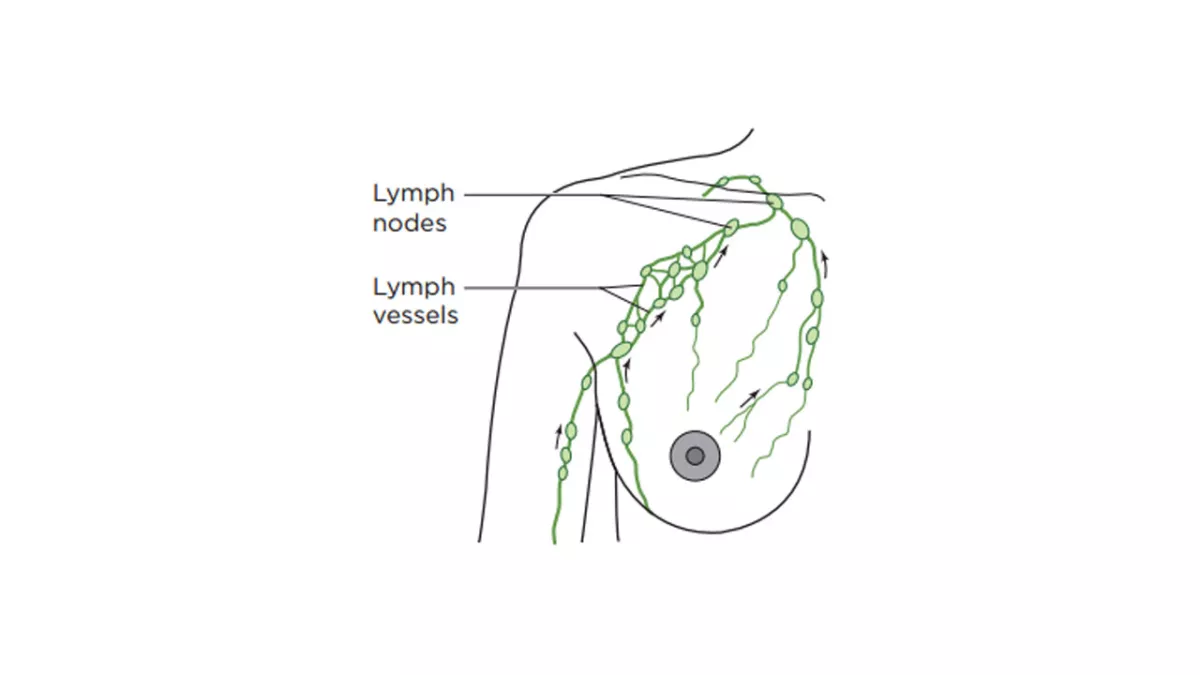
\includegraphics[width=\textwidth]{../figs/introduction/lymphatic_system_in_a_breast.png}
                        \caption{Lymphatic System Overview \cite{RefWorks:RefID:37-memorialsurgery}.}
                        \label{fig:introduction:lymphatic_system_in_a_breast}
                \end{subfigure}
                \begin{subfigure}[b]{0.45\textwidth}
                        \centering
                        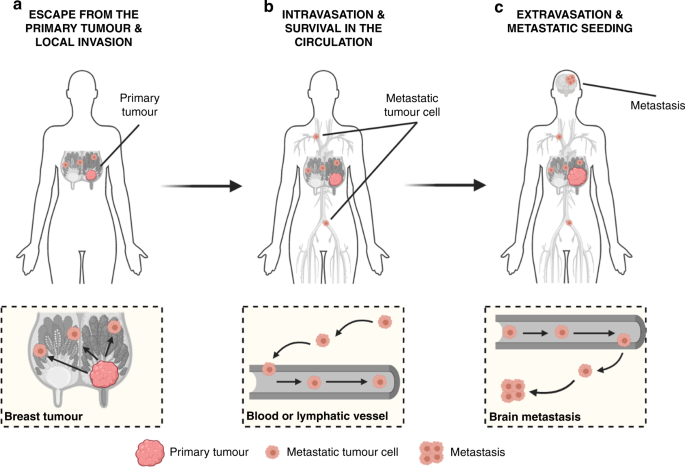
\includegraphics[width=\textwidth]{../figs/introduction/process_of_metastatic_breast_cancer.png}
                        \caption{Lymph Nodes Overview \cite{RefWorks:RefID:364-riggio2020lingering}.}
                        \label{fig:introduction:lymphatic_process_of_metastatic_breast_cancer}
                \end{subfigure}
        \end{minipage}
        \caption{Lymphatic System and Lymph Nodes Overview \cite{RefWorks:RefID:364-riggio2020lingering} \cite{RefWorks:RefID:37-memorialsurgery}.}
        \label{fig:introduction:lymphatic_system_and_nodes_overview}
\end{figure}

\subsection{Treatment of Breast Cancer\label{sec:introduction:treatmentofbreastcancer}}

\subsubsection{Stages of Breast Cancer\label{sec:introduction:breastcancer:stagesofbreastcancer}}
% Early vs late stage
Breast cancer is classified in stages ranging from 0 to IV based on the cancer's characteristics such as tumor size~\cite{RefWorks:RefID:151-2025breast}.

Stage 0 breast cancer is described as non-invasive, meaning the cancer cells are confined to the ducts or lobules in the breast and have not spread to surrounding healthy tissue~\cite{RefWorks:RefID:151-2025breast}.

Stage I breast cancer is invasive, meaning the cancer cells have spread to surrounding healthy tissue. In stage I breast cancer, the tumor is up to 2cm in size but invading cancer cells are no more than 1mm. Stage I is classified as either IA or IB depending on the sevarity of the cancer.~\cite{RefWorks:RefID:151-2025breast}.

Stage II breast cancer is used when the cancer is larger than 2cm but no larger than 5cm, or if the cancer has spread to one to three nearby lymph nodes. Similar to stage I breast cancer, stage II breast cancer can be subdivided into IIA and IIB~\cite{RefWorks:RefID:151-2025breast}.

Stage II breast cancer can be divided into IIIA, IIIB, and IIIC. This stage describes invasive breast cancer that is larger than 5cm or is found in four to nine nearby lymph nodes (IIIA), has spread to the chest wall or skin of the breast (IIIB), or has spread to ten or more nearby lymph nodes or to lymph nodes above or below the collarbone (IIIC)~\cite{RefWorks:RefID:151-2025breast}.

Lastly, stage IV breast cancer describes cancer that has metastasized, or spread, to other parts of the body such as the lungs, liver, bones, or brain~\cite{RefWorks:RefID:151-2025breast}.

Breast cancer stages can be divided into early and late stage breast cancer. Early-stage breast cancer incudes stages 0, I, and IIA while late-stage breast cancer includes stages IIB, III, and IV~\cite{RefWorks:RefID:365-stages}. Table~\ref{tab:introduction:breastcancer:stages} summarizes the stages of breast cancer. An overview of breast cancer treatment options for early and late stage breast cancer is shown in Figure~\ref{fig:introduction:breast_cancer_treatment_options_overview}.


\begin{table}[h!]
        \centering
        \caption{Stages of Breast Cancer~\cite{RefWorks:RefID:151-2025breast, RefWorks:RefID:365-stages}.}
        \label{tab:introduction:breastcancer:stages}
        \begin{tabular}{|c|c|c|}
                \hline
                \textbf{Stage} & \textbf{Description}                                       & \textbf{Early/Late Stage} \\
                \hline
                0              & Non-invasive, confined to ducts or lobules                 & Early                     \\
                \hline
                I              & Invasive, tumor up to 2cm, invading cells no more than 1mm & Early                     \\
                \hline
                IIA            & Tumor 2-5cm or spread to 1-3 lymph nodes                   & Early                     \\
                \hline
                IIB            & Tumor larger than 5cm or spread to 1-3 lymph nodes         & Late                      \\
                \hline
                IIIA           & Tumor larger than 5cm or found in 4-9 lymph nodes          & Late                      \\
                \hline
                IIIB           & Spread to chest wall or skin of breast                     & Late                      \\
                \hline
                IIIC           & Spread to 10+ lymph nodes or above/below collarbone        & Late                      \\
                \hline
                IV             & Metastasized to other parts of the body                    & Late                      \\
                \hline
        \end{tabular}
\end{table}

\subsubsection{Current Treatment Options\label{sec:introduction:breastcancer:currenttreatmentoptions}}

\subsubsection*{Surgical Options\label{sec:introduction:breastcancer:currenttreatmentoptions:surgicaloptions}}

Treatment options for breast cancer largely depend on the type and stage of the cancer. Surgical choices include a lumpectomy, which removes the tumor and a small margin of surrounding healthy tissue, or a mastectomy, which removes the entire breast~\cite{RefWorks:RefID:165-czajka2023breast}.

A lumpectomy is followed by radiation therapy to kill any stray cancer cells that may remain in the breast. This combination helps lower the risk of recurrence, or the return of the cancer~\cite{RefWorks:RefID:159-depolo2024radiation}. Radiation therapy is performed using high-energy X-rays to damage a cancer cell's DNA, preventing it from dividing further until it dies. Healthy tissue cells grow and divide slower than cancer cells, allowing them to repair themselves after radiation therapy while cancer cells cannot~\cite{RefWorks:RefID:159-depolo2024radiation}. See Section~\ref{sec:introduction:radiationtherapy} for more information on radiation therapy.

\subsubsection*{Lymph Node Biopsy\label{sec:introduction:breastcancer:currenttreatmentoptions:lymphnodebiopsy}}
In most surgical treatments for breast cancer, a lymph node biopsy is performed to check if cancer has spread past the breast tissue and to the lymph nodes. Samples from one or more lymph nodes are removed and examined under a microscope for cancer cells~\cite{RefWorks:RefID:37-memorialsurgery}. Standard practice was removing most of the lymph nodes in the underarm, called an axillary dissection. Today, a sentinel lymph node biopsy is more commonly performed to allow a faster recovery time~\cite{RefWorks:RefID:37-memorialsurgery}.

\subsubsection*{Sentinel Lymph Node Biopsy\label{sec:introduction:breastcancer:currenttreatmentoptions:sentinellymphnodebiopsy}}
The sentinel lymph node is the first lymph node that breast cancer cells spread to after leaving the breast. In a sentinel lymph node biopsy, a radioactive tracer (often technetium-99m) and/or a blue dye is injected into the side of the tumor. The tracer(s) travel through the lymphatic system to the sentinel lymph node. The blue stain and radiotracer signal, found with a gamma probe, can be used to identify and excise this lymph node for examination under a microscope for cancer cells~\cite{RefWorks:RefID:37-memorialsurgery},~\cite{RefWorks:RefID:165-czajka2023breast}.

\subsubsection*{Systemic Therapies\label{sec:introduction:breastcancer:currenttreatmentoptions:systemictherapies}}
While breast cancer treatment commonly starts with surgery, systemic therapies such as chemotherapy, hormone therapy, or targeted therapies may also be used~\cite{RefWorks:RefID:37-memorialsurgery}.

Chemotherapy, often called "chemo," uses strong medicines to slow or stop cancer cells from growing further. As chemotherapy often works by attacking cells that divide quickly, it can attack cancer cells but also other healthy cells that divide quickly such as those that make your hair grow. This can lead to side effects such as hair loss and nausea~\cite{RefWorks:RefID:37-memorialsurgery}.

Hormone treatment is used for breast cancer cells that require hormones such as estrogen to grow. This is done by blocking the hormones these cancer cells need to grow. Side effects can include changes in menstrual cycle, hot flashes, and aching bones~\cite{RefWorks:RefID:37-memorialsurgery}.

Targeted therapies, or precision medicines, attack specific characteristics of an individual's cancer cells rather than attacking all rapidly dividing cells like chemotherapy. Targeted therapies can treat the most common breast cancer gene mutations such as BRCA1 and BRCA2, HER2, and PIK3CA. This individualized treatment can lead to less side effects than in chemotherapy~\cite{RefWorks:RefID:37-memorialsurgery}.

\begin{figure}[h!]
        \centering
        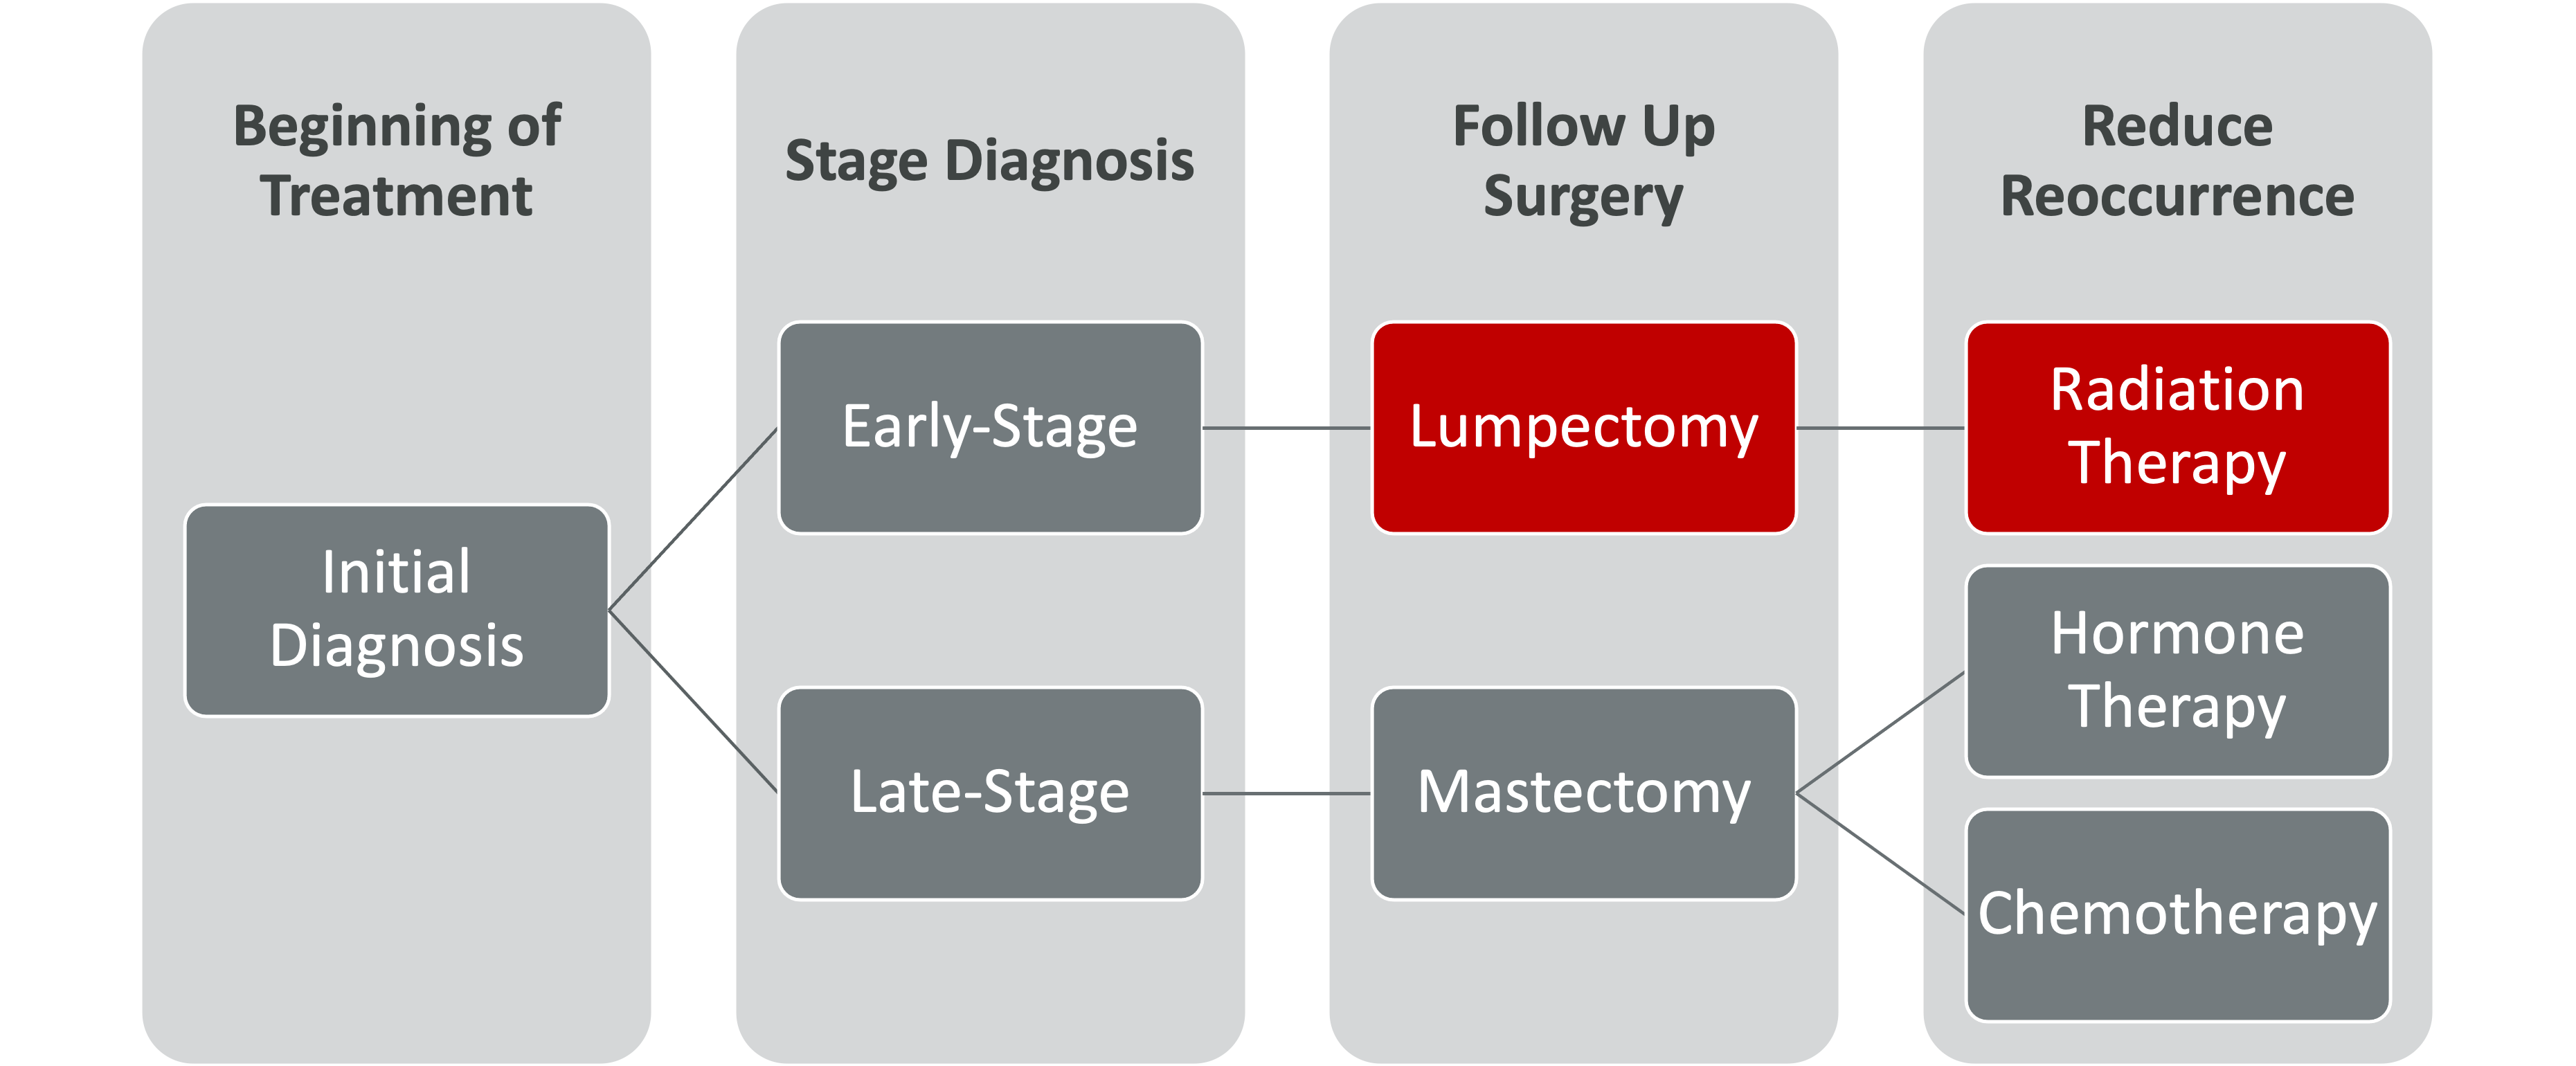
\includegraphics[width=0.6\textwidth]{../figs/introduction/breast_cancer_treatment_process_flowchart.png}
        \caption{Breast Cancer Treatment Options Overview \cite{RefWorks:RefID:37-memorialsurgery}, \cite{RefWorks:RefID:370-einsteinisaac}.}
        \label{fig:introduction:breast_cancer_treatment_options_overview}
\end{figure}

\subsection{Radiation Therapy\label{sec:introduction:radiationtherapy}}
\subsubsection{Radiation Therapy Overview\label{sec:introduction:radiationtherapy:overview}}
As mentioned in Section~\ref{sec:introduction:breastcancer:currenttreatmentoptions:surgicaloptions}, radiation therapy often follows a lumpectomy procedure to kill any stray cancer cells and prevent the cancer from resurfacing. Together, a lumpectomy procedure followed by radiation therapy is commonly known as breast-conserving therapy (BCT). Some compare breast cancer surgery to picking up the large pieces of a broken glass off the floor, while radiation therapy is like vacuuming the remaining shards at the end.

Including radiation therapy after a lumpectomy has been shown to reduce the risk of ipsilateral (same side) recurrence as well as increase overall survival rates~\cite{RefWorks:RefID:157-thomasscience}, ~\cite{RefWorks:RefID:198-jiao2024interobserver}.

\subsubsection{Whole vs Accelerated Partial Breast Irradiation\label{sec:introduction:radiationtherapy:wholevsacceleratedpartialbreastirradiation}}
Patients undergoing BCT can receive either whole breast irradation (WBI) or accelerated partial breast irradiation (APBI). WBI is the more common of the two techniques, although APBI has been gaining traction in recent years due to its unique benefits~\cite{RefWorks:RefID:157-thomasscience}.

WBI is delivered over the course of five to six weeks while APBI is delivered over the course of one week. APBI also limits radiation exposure to 1-2 cm margin of healthy tissue surrounding the tumor site. This limited exposure reduces radiation exposure risks to surrounding organs such as lungs, heart, or ribs. APBI also resulted in higher rates of "excellent/good" cosmetic outcomes compared to WBI (81\% vs 63\% respectively)~\cite{RefWorks:RefID:157-thomasscience}. Comparison of radiation exposure in WBI vs APBI is illustrated in Figure~\ref{fig:introduction:WBI_vs_APBI_irradiation_comparison}.

\begin{figure}[h!]
        \centering
        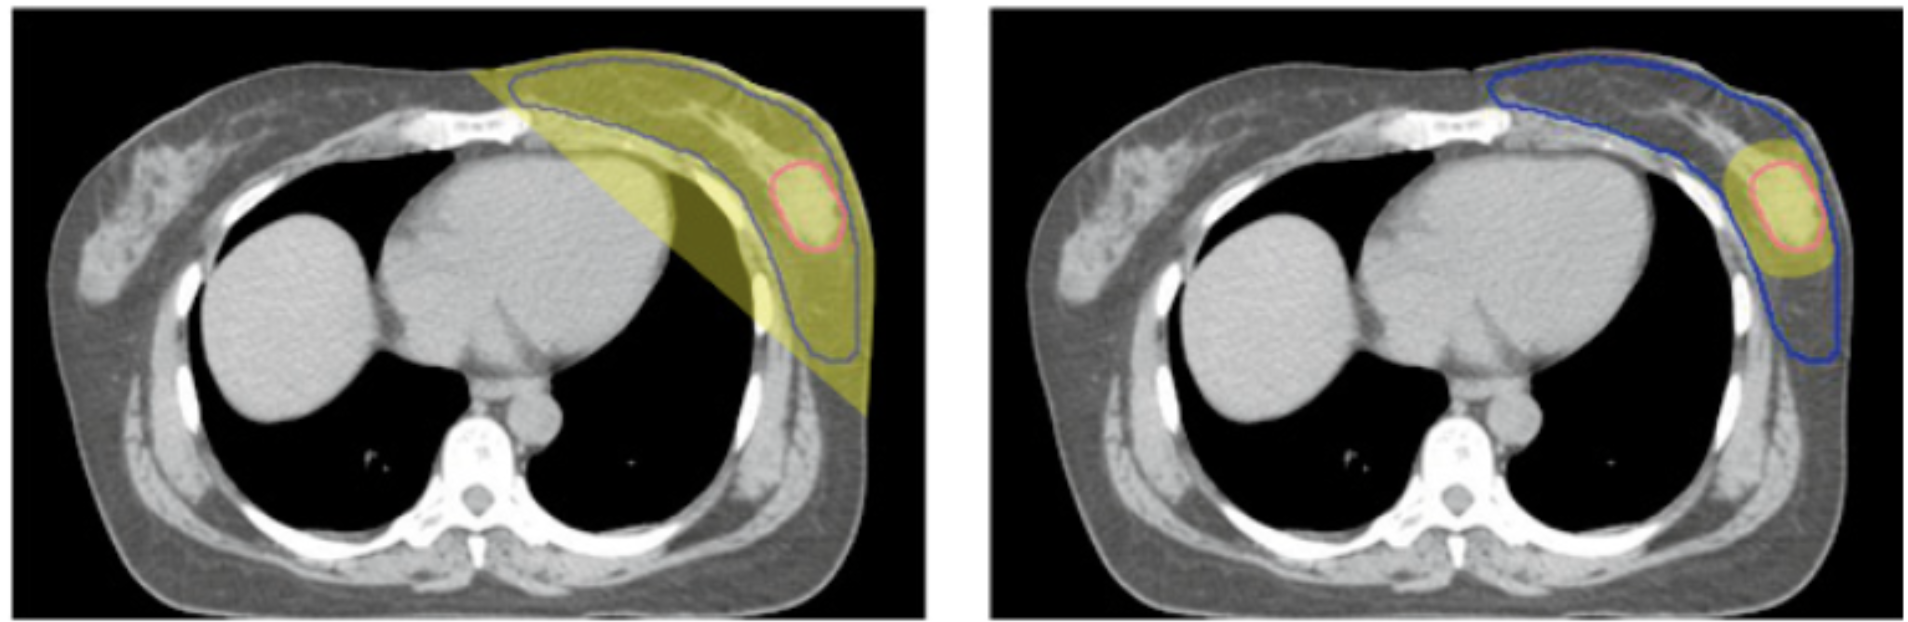
\includegraphics[width=0.6\textwidth]{../figs/introduction/WBI_vs_APBI_irradiation_comparison.png}
        \caption{Comparison of radiation exposure between Whole Breast Irradiation (WBI) (left) and Accelerated Partial Breast Irradiation (APBI) (right) \cite{RefWorks:RefID:157-thomasscience}. The yellow area indicates the irradiated region.}
        \label{fig:introduction:WBI_vs_APBI_irradiation_comparison}
\end{figure}

\subsubsection{Radiation Therapy Treatment Planning\label{sec:introduction:radiationtherapy:treatmentplanning}}
Radiation therapy (WBI or APBI) requires tumor bed delineation to identify and outline the tumor as well as a surrounding healthy tissue margin. This treatment planning ensures radiation is delivered accurately to the tumor site while minimizing exposure to healthy surrounding tissue and organs~\cite{RefWorks:RefID:197-den2015postlumpectomy}.

One concern with tumor bed (TB) delineation is the interobserver variability in accurately marking the TB~\cite{RefWorks:RefID:197-den2015postlumpectomy},~\cite{RefWorks:RefID:179-yang2013tumor}. There are many methods and devices used to assist in TB delineation to address these concerns such as surgical clips, pre-operative imaging, seroma formation, fiducial markers, and other implantable devices~\cite{RefWorks:RefID:179-yang2013tumor},~\cite{RefWorks:RefID:25-acree2022review}.

\subsection{Motivation\label{sec:introduction:motivation}}
The motivation for this work stems from the need to standardize and improve the accuracy and consistency of tumor bed (TB) delineation in radiation therapy following a lumpectomy procedure.

The challenges with accurate TB delineation following a lumpectomy procedure arise because the cancerous tissue has been removed, leaving behind a tumor cavity that is difficult to accurately trace~\cite{RefWorks:RefID:25-acree2022review}. Additionally, unlike other parts of the body, the breast lacks anatomic landmarks to assist with tumor bed delineation~\cite{RefWorks:RefID:344-mitchell2019adaptable}. This need for a marking method is visualized below in Figure~\ref{fig:introduction:need_for_tumor_bed_marker}.

\begin{figure}[h!]
        \centering
        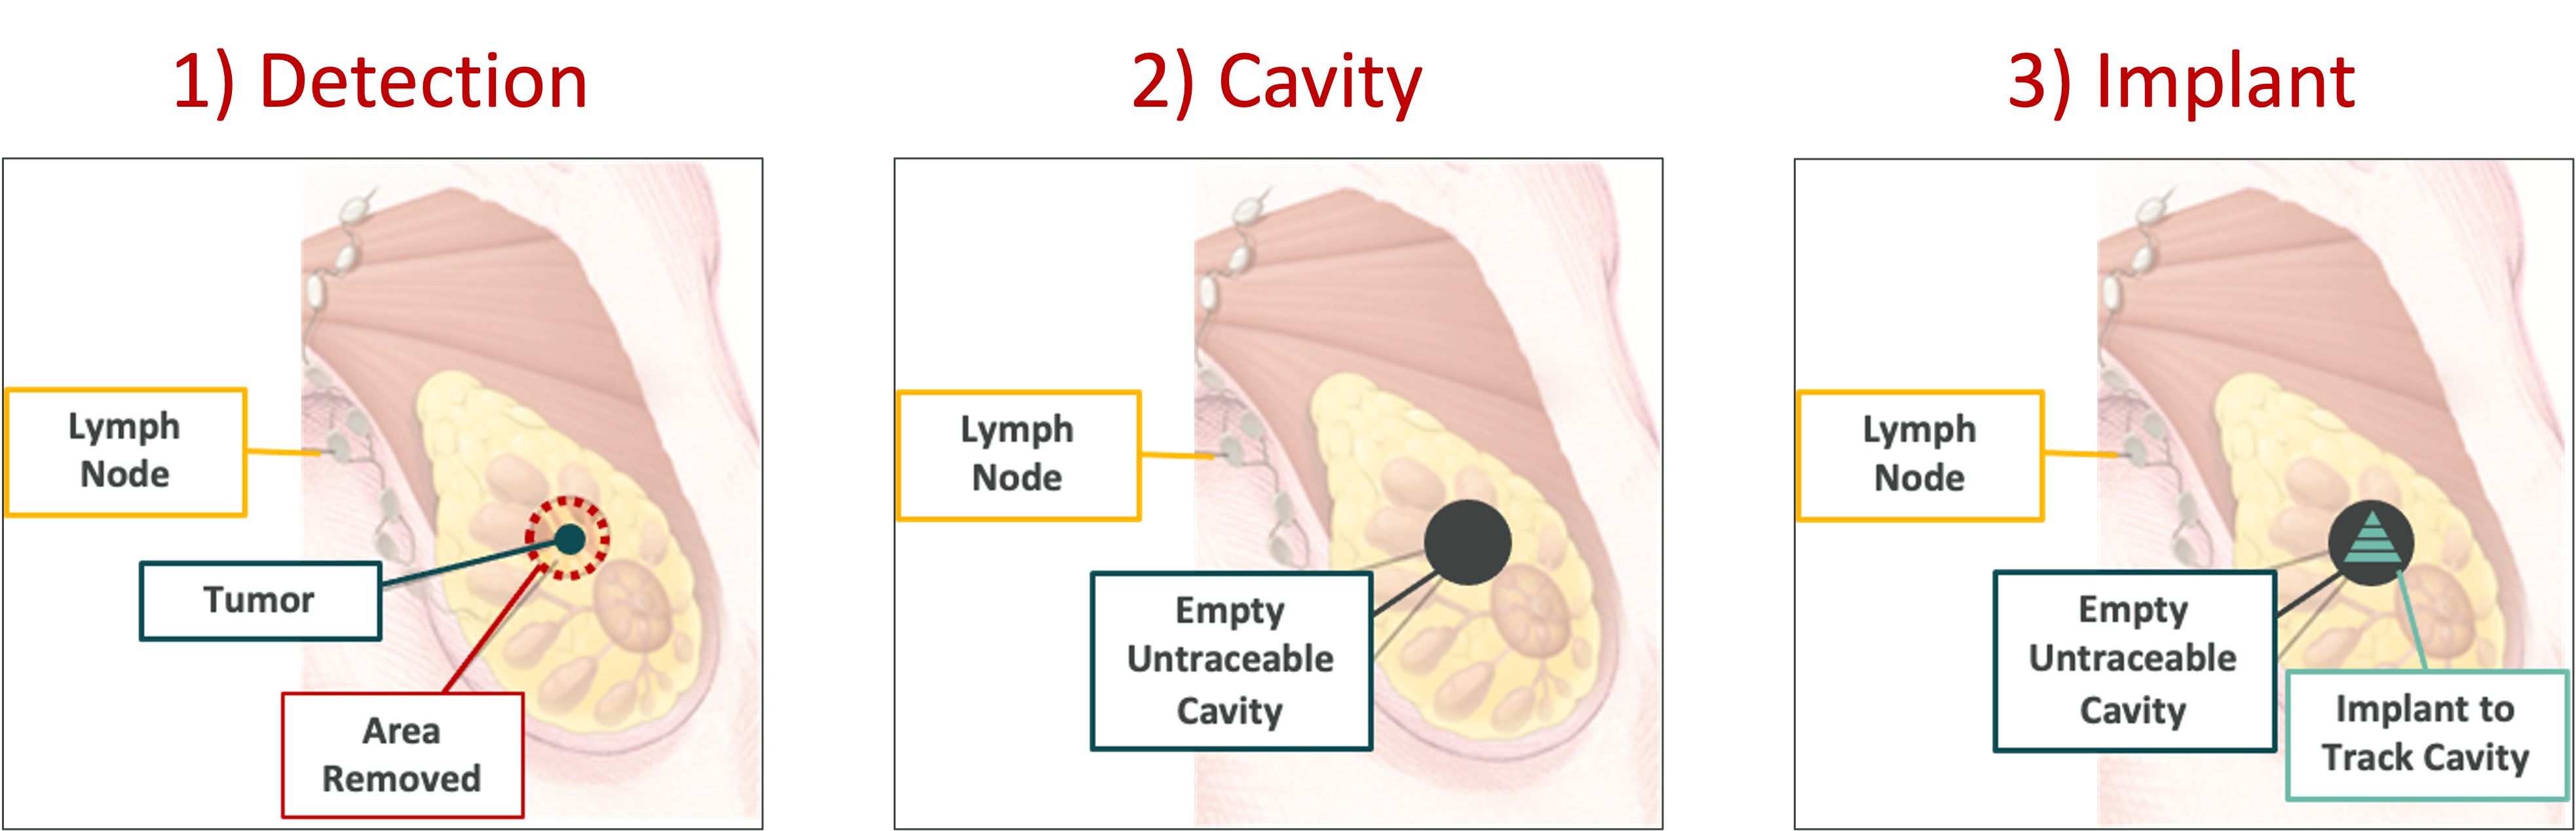
\includegraphics[width=0.6\textwidth]{../figs/introduction/need_for_tumor_bed_marker.png}
        \caption{Motivation for tumor cavity marker following lumpectomy procedure. Adapted from \cite{RefWorks:RefID:38-johnbreastconserving}.}
        \label{fig:introduction:need_for_tumor_bed_marker}
\end{figure}

Current devices and methods used for TB delineation have limitations that affect the overall consistency and accuracy of post-lumpectomy radiation therapy. As over 70\% of breast cancer recurrences occur at the original tumor site, accurate TB delineation and radiation delivery is important in improving patient outcomes~\cite{RefWorks:RefID:25-acree2022review}.

\subsubsection{Importance of Accurate Tumor Bed Delineation\label{sec:introduction:motivation:importanceofaccuratetumorbeddelineation}}
\hl{See if this could use more detail.\\}
Accurate TB delineation is crucial in effective radiation therapy following a lumpectomy procedure given the increasing use of APBI. Since APBI targets a small area of tissue surrounding the tumor bed, accurate delineation is necessary to ensure the radiation dose is delivered precisely to the intended area while minimizing exposure to surrounding healthy tissue and organs~\cite{RefWorks:RefID:197-den2015postlumpectomy}, ~\cite{RefWorks:RefID:25-acree2022review}.

Overestimating TB volume, common in seroma-based delineation, is associated with an increased risk of subcutaneous fibrosis and poorer cosmetic results~\cite{RefWorks:RefID:197-den2015postlumpectomy}. Conversely, underestimating TB volume can lead to insufficient radiation coverage of the tumor bed, increasing the risk of local recurrence~\cite{RefWorks:RefID:198-jiao2024interobserver}. An inaccurate TB volume can
also lead to alteration of management of a radiation boost and completely missing one or more margins of the TB~\cite{RefWorks:RefID:344-mitchell2019adaptable}.

\subsubsection{Current Devices and Methods\label{sec:introduction:motivation:currentdevicesandmethods}}
\hl{See if this could use more detail.\\}
Current devices and methods used for TB delineation include titanium, gold, or liquid fiducial markers/surgical clips, surgeon discretion, seroma formation, or implantable devices~\cite{RefWorks:RefID:25-acree2022review}.

Fiducial markers are solid metal clips inserted around the border of a tumor cavity immediately following the tumor removal~\cite{RefWorks:RefID:358-defining}. These provide a 2D point mapping of the tumor space as shown below in Figure~\ref{fig:introduction:imaging_of_fiducal_clips_in_phantom_breast}.

Liquid fiducial markers were first used as spacers for prostate cancer treatment planning. They have since been repurposed to be used for TB delineation. These markers provide a clearer delineation than solid clips as they conform to the tumor cavity shape~\cite{RefWorks:RefID:25-acree2022review}.

\begin{figure}[h!]
        \centering
        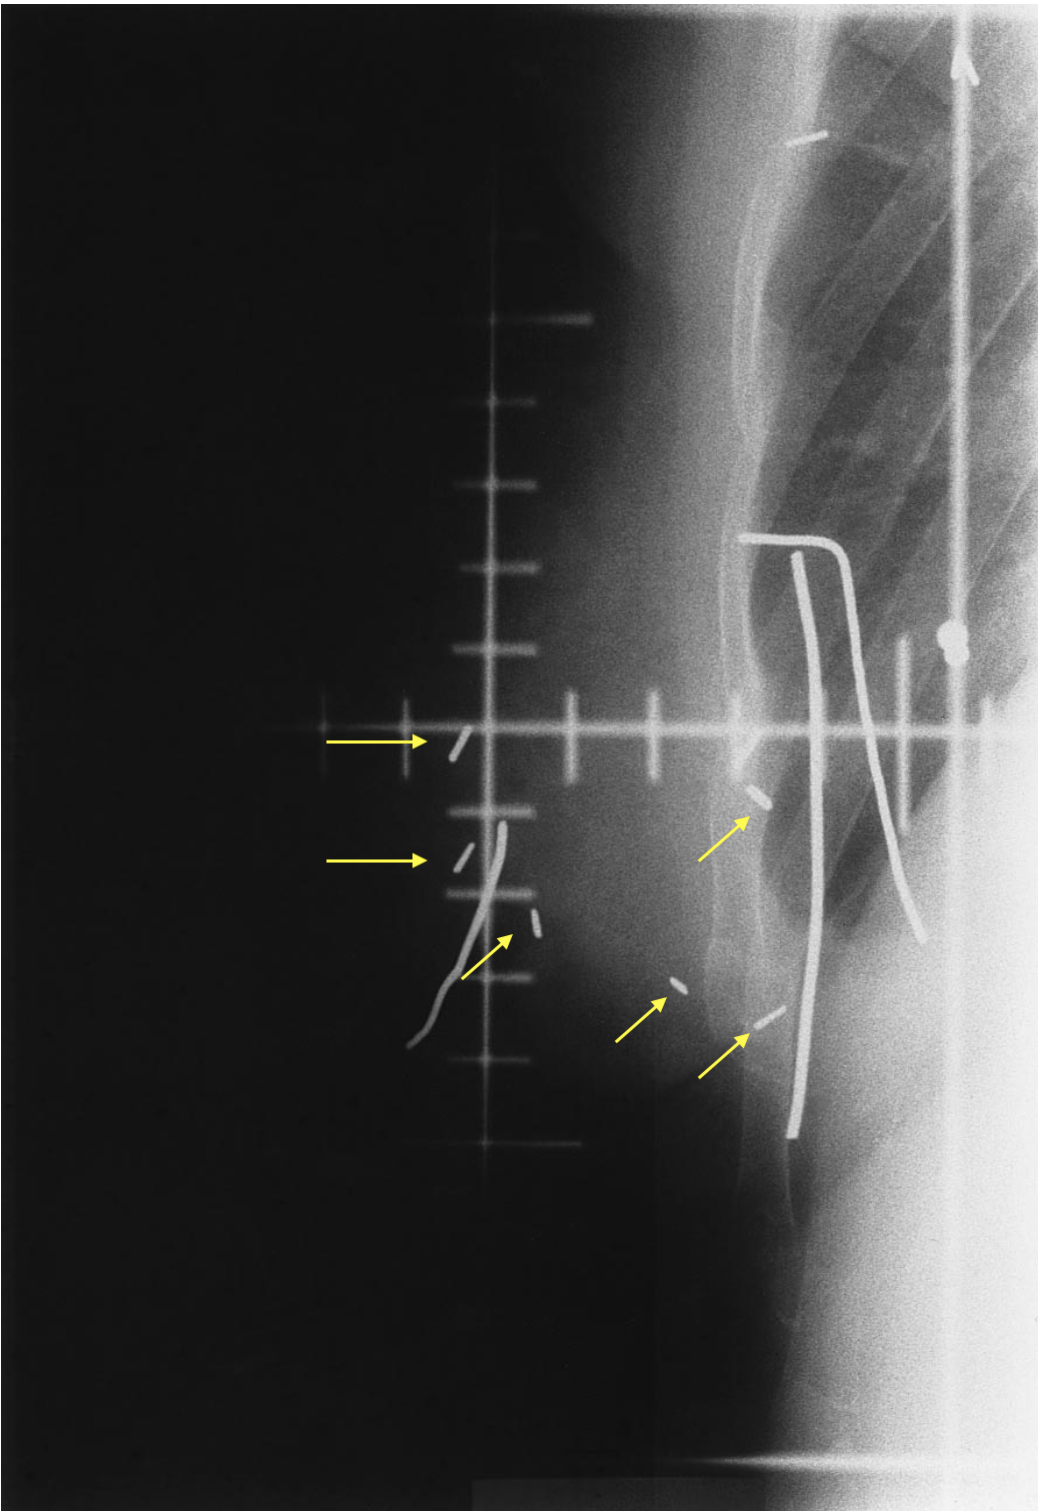
\includegraphics[width=0.6\textwidth]{../figs/introduction/imaging_of_fiducal_clips_in_phantom_breast.png}
        \caption{Imaging of Fiducial Clips in Phantom Breast. Yellow arrows indicate fiducial clips placed around tumor cavity. Adapted from \cite{RefWorks:RefID:178-krawczyk1994importance}.}
        \label{fig:introduction:imaging_of_fiducal_clips_in_phantom_breast}
\end{figure}

Using seroma formation to mark the tumor bed for radiation therapy involves outlining the seroma that forms following a lumpectomy procedure~\cite{RefWorks:RefID:25-acree2022review}.

Lastly, implantable devices can be used to mark the tumor bed. One example is BioZorb (Hologic) which is a 3-dimensional coil-like structure with titanium clips embedded. This device is implanted into the tumor cavity following a lumpectomy procedure and improves on titanium clips alone by creating a 3D outline of the tumor bed. BioZorb was also designed to be reabsorbed into the body within a year~\cite{RefWorks:RefID:25-acree2022review}. BioZorb is shown below in Figure~\ref{fig:introduction:biozorb_implant}.

\begin{figure}[h!]
        \begin{minipage}{0.92\textwidth}
                \centering
                \begin{subfigure}[b]{0.9\textwidth}
                        \centering
                        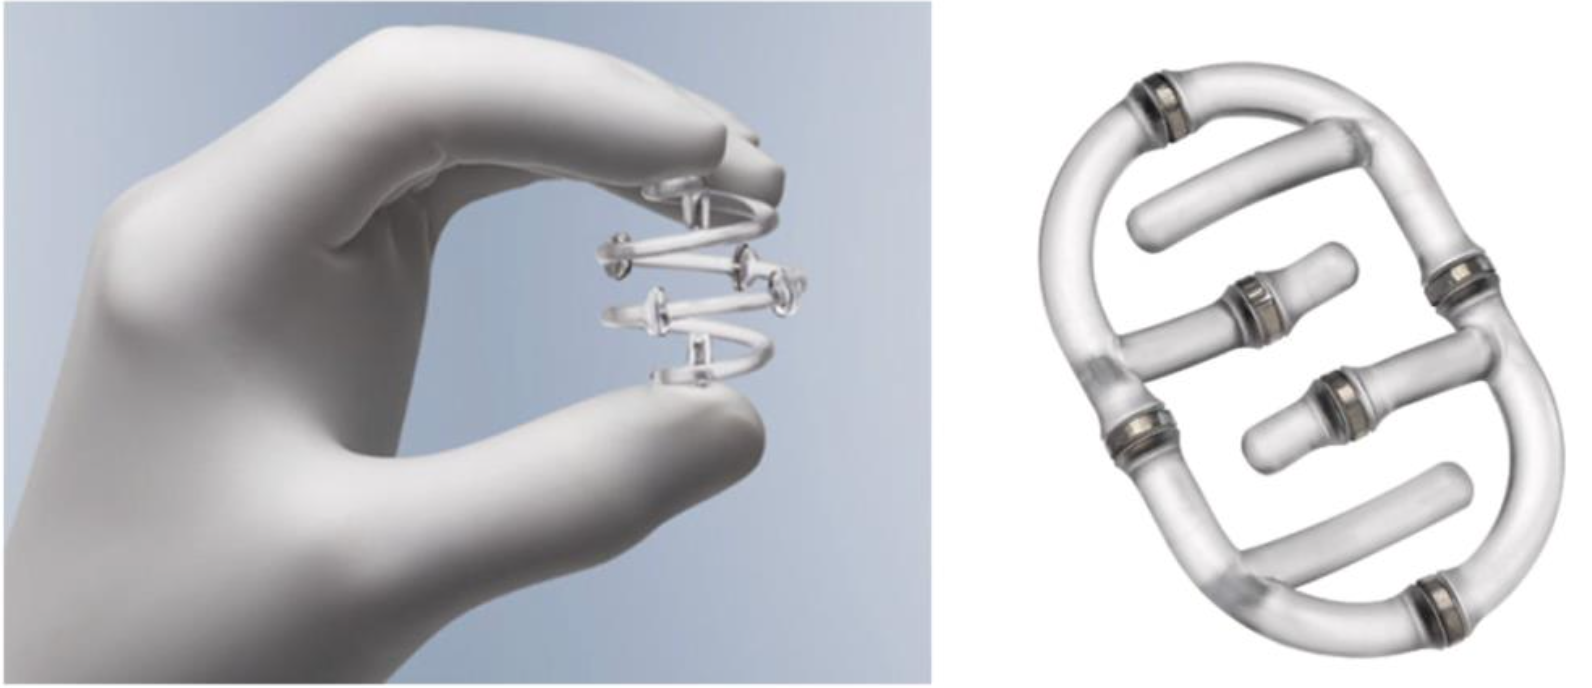
\includegraphics[width=\textwidth]{../figs/introduction/BioZorb_physically.png}
                        \caption{BioZorb physically (top).}
                        \label{fig:introduction:biozorb_physically}
                \end{subfigure}

                \vspace{1em} % optional space between images

                \begin{subfigure}[b]{0.9\textwidth}
                        \centering
                        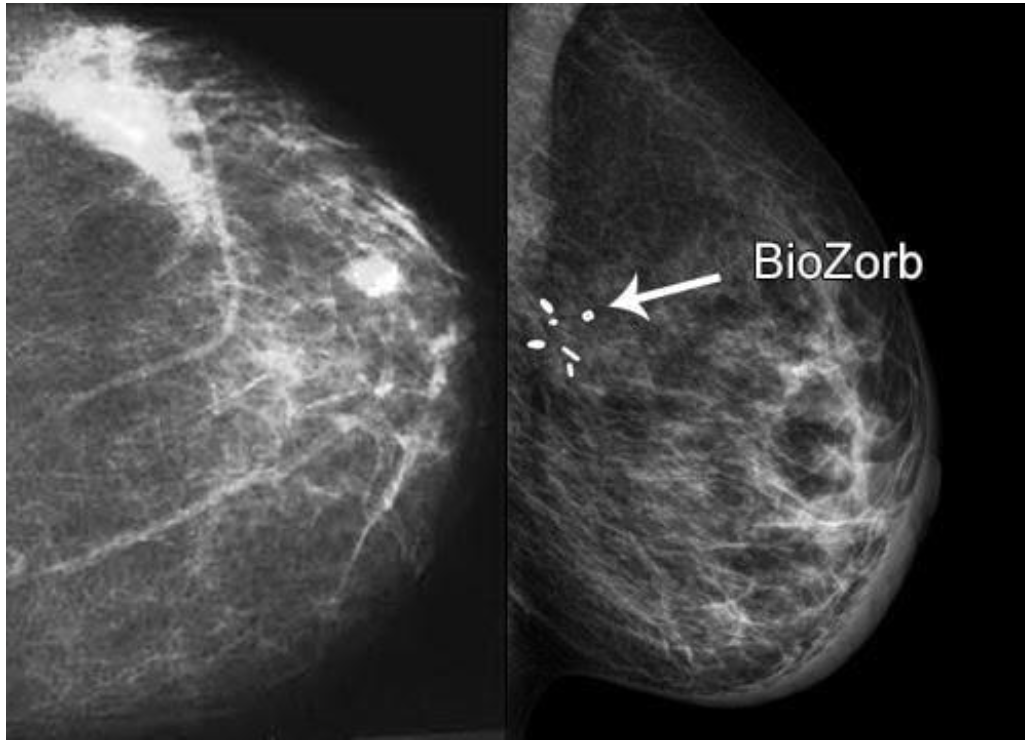
\includegraphics[width=\textwidth]{../figs/introduction/BioZorb_in_imaging.png}
                        \caption{BioZorb in imaging.}
                        \label{fig:introduction:biozorb_in_imaging}
                \end{subfigure}
        \end{minipage}
        \caption{BioZorb, an implantable device to assist with TB delineation~\cite{RefWorks:RefID:370-einsteinisaac}.}
        \label{fig:introduction:biozorb_implant}
\end{figure}

A newer implantable device is Veraform, a continuously radiographically opaque filament that is stitched around the tumor cavity. By being malleable and sewn in place, this device addresses space limitations and migration issues present in other devices~\cite{RefWorks:RefID:344-mitchell2019adaptable}. A simulation showing Veraform in use is shown below in Figure~\ref{fig:introduction:veraform_implant}.
\begin{figure}[h!]
        \centering
        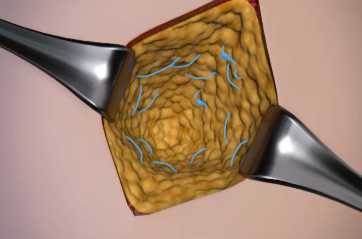
\includegraphics[width=0.6\textwidth]{../figs/introduction/veraform_implant.png}
        \caption{Veraform, an implantable device to assist with TB delineation~\cite{RefWorks:RefID:344-mitchell2019adaptable}.}
        \label{fig:introduction:veraform_implant}
\end{figure}

\subsubsection{Challenges with Current Devices and Methods\label{sec:introduction:motivation:challengeswithcurrentdevicesandmethods}}
\hl{See if this could use more detail.\\}

\subsubsection*{Challenges with Fiducial Markers\label{sec:introduction:motivation:challengeswithcurrentdevicesandmethods:challengeswithfiducialmarkers}}
There are many challenges and inaccuracies that can result from using fiducial markers or surgical clips to create a TB volume. They provide single points of reference which can lead to inaccurate boundaries being drawn, there is no standardized recommendation of how many clips should be used, and clips can migrate over time leading to inaccurate TB localization~\cite{RefWorks:RefID:344-mitchell2019adaptable}. Migration is especially common when patients undergo oncoplastic reconstruction surgery following the lumpectomy procedure. In 2022, it was found the 30,000 breast-conserving therapy patients annually undergo oncoplastic reconstruction surgery~\cite{RefWorks:RefID:25-acree2022review}.

Another concern of surgical clips or fiducial markers is if a re-excision is required. This is when a margin of tissue removed during the lumpectomy is found to contain cancerous cells. When this is the case, a large enough margin surrounding the tumor was not removed, and a re-excision has to be made to remove additional margins. When markers are placed initially, these re-excisions can impact the accuracy of the initial marker placement. It was found that 10\% to 20\% of patients undergoing breast-conserving surgery require a re-excision~\cite{RefWorks:RefID:25-acree2022review}.

\subsubsection*{Challenges with Seroma Formation\label{sec:introduction:motivation:challengeswithcurrentdevicesandmethods:challengeswithseromaformation}}
\hl{Show change in seroma over time visual.\\}

Utilizing seroma formation can be unreliable, as the seroma may not always be localized to the tumor bed, relies on the excision closure method, and time elapsed after surgery\cite{RefWorks:RefID:25-acree2022review}. A seroma may represent the tumor bed, part of the tumor bed, or the entire area in which surgery was performed~\cite{RefWorks:RefID:344-mitchell2019adaptable}.

\subsubsection*{Challenges with Biozorb}
Biozorb was found to provide limited value to patients relative to its high cost~\cite{RefWorks:RefID:344-mitchell2019adaptable}. Additionally, Biozorb was also recalled due to patient discomfort, seroma formation, device migration, and failures to resorb into the body in the designated timeframe~\cite{RefWorks:RefID:296-2024hologic},~\cite{RefWorks:RefID:28-nudelunited}.

\subsubsection{Proposed Solution\label{sec:introduction:motivation:proposedsolution}}
% Explain our research and the proposed mesh


\section{Design\label{chapthree:design}}

\lipsum{}

%%% Local Variables:
%%% mode: latex
%%% TeX-master: "../dissertation"
%%% End:


\section{Implementation\label{chap1:impl}}


%%% Local Variables:
%%% mode: latex
%%% TeX-master: "../dissertation"
%%% End:


\section{Evaluation\label{chap1:eval}}

%%% Local Variables:
%%% mode: latex
%%% TeX-master: "../dissertation"
%%% End:


\chapter{Conclusion\label{chap:conclusion}}

\if@ms
In this chapter, we summarize the status of the work presented in this proposal, and outline future plans~\cite{template}.
\else
In this chapter, we summarize the status of the work presented in this dissertation, and outline future plans~\cite{template}.
\fi

\section{Summary\label{sec:conclusion:summary}}

\lipsum{}

\section{Contributions\label{sec:conclusion:contributions}}

\lipsum{}


    \chapter{Contribution 3\label{chap:contrib3}}

\lipsum{}

%%% Local Variables:
%%% mode: latex
%%% TeX-master: "../dissertation"
%%% End:


\newpage
\section{Background\label{introduction:background}}

\subsection{Breast Cancer Overview\label{sec:introduction:breastcanceroverview}}
Breast cancer is a type of cancer that starts in one or both breasts. The left and right breast are each mainly glands, ducts, and fatty tissue. Breast cancer can start in these different parts of the breast or others~\cite{RefWorks:RefID:36-american2021breast}.

\subsubsection{Statistics\label{sec:introduction:breastcancer:statistics}}
Breast cancer accounts for about 30\% of all new cancer cases in U.S. women each year~\cite{RefWorks:RefID:150-2025breast}. The average risk of a woman in the U.S. developing breast cancer sometime in her life is about 1 in 8 (about 13\%)~\cite{RefWorks:RefID:36-american2021breast}. Breast cancer is also the second leading cause of cancer death in women behind lung cancer~\cite{RefWorks:RefID:36-american2021breast}.

\subsubsection{Development and Spread\label{sec:introduction:breastcancer:developmentandspread}}
Breast cancer can start in different parts of the breast, such as the ducts, lobules, or the tissue in between. The cancer can spread when cancer cells are carried to other parts of the body through blood or the lymphatic system. The lymphatic system is a network of small bean-sized glands called lymph nodes, ducts, and vessels that carry clear lymph fluid throughout the body. This clear lymph fluid contains immune system cells to fight infection as well as waste and tissue by-products. This system carries lymph fluid away from the breast; cancer cells can enter the lymph vessels, grow inside lymph nodes, and spread to other parts of the body~\cite{RefWorks:RefID:36-american2021breast}.

The most common areas where lymph vessels of the breast drain into are the underarm (axillary), inside the chest near the breastbone (internal mammary), and around the collar bone (supraclavicular and infraclavicular). Once cancer cells have spread to  the lymph nodes, there is a higher chance of metastases, or spreading, to other parts of the body which is called metastatic breast cancer~\cite{RefWorks:RefID:36-american2021breast}.

The method of cancer cells metastasizing through the lymphatic system is illustrated below in Figure~\ref{fig:introduction:lymphatic_system_in_a_breast} and Figure~\ref{fig:introduction:lymphatic_process_of_metastatic_breast_cancer}.

\begin{figure}[h!]
        \begin{minipage}{0.92\textwidth}
                \centering
                \begin{subfigure}[b]{0.45\textwidth}
                        \centering
                        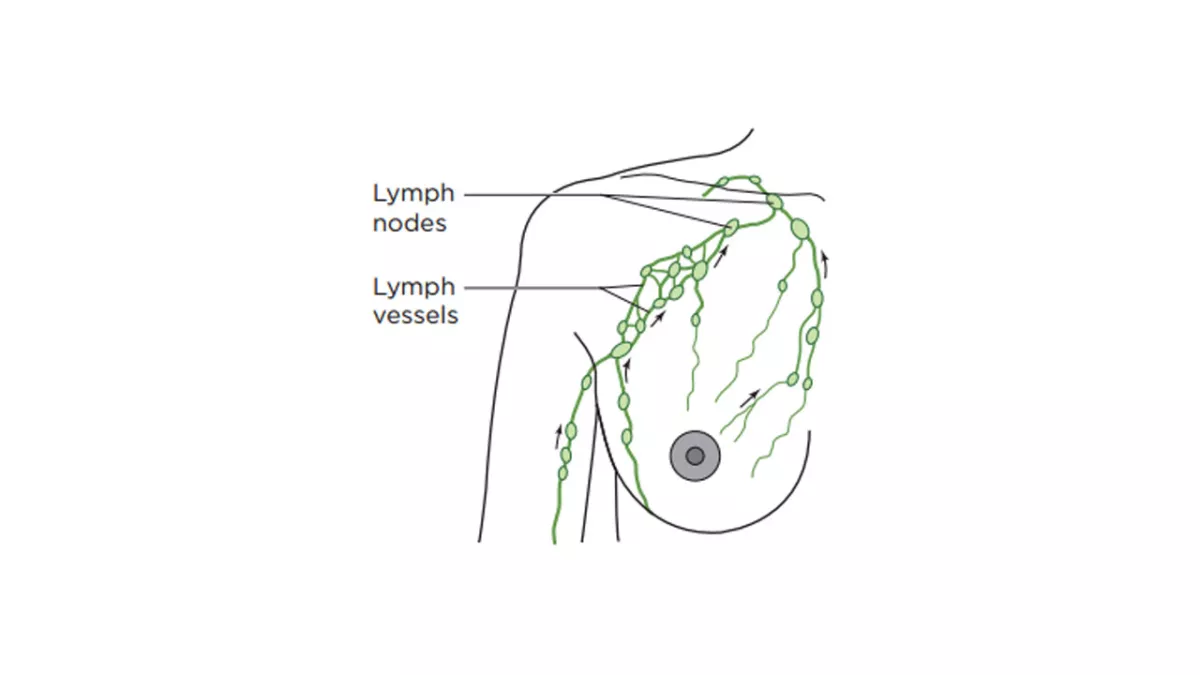
\includegraphics[width=\textwidth]{../figs/introduction/lymphatic_system_in_a_breast.png}
                        \caption{Lymphatic System Overview \cite{RefWorks:RefID:37-memorialsurgery}.}
                        \label{fig:introduction:lymphatic_system_in_a_breast}
                \end{subfigure}
                \begin{subfigure}[b]{0.45\textwidth}
                        \centering
                        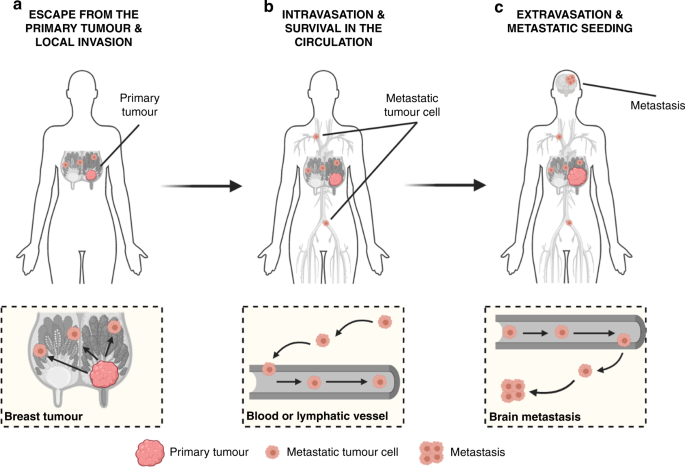
\includegraphics[width=\textwidth]{../figs/introduction/process_of_metastatic_breast_cancer.png}
                        \caption{Lymph Nodes Overview \cite{RefWorks:RefID:364-riggio2020lingering}.}
                        \label{fig:introduction:lymphatic_process_of_metastatic_breast_cancer}
                \end{subfigure}
        \end{minipage}
        \caption{Lymphatic System and Lymph Nodes Overview \cite{RefWorks:RefID:364-riggio2020lingering} \cite{RefWorks:RefID:37-memorialsurgery}.}
        \label{fig:introduction:lymphatic_system_and_nodes_overview}
\end{figure}

\subsection{Treatment of Breast Cancer\label{sec:introduction:treatmentofbreastcancer}}

\subsubsection{Stages of Breast Cancer\label{sec:introduction:breastcancer:stagesofbreastcancer}}
% Early vs late stage
Breast cancer is classified in stages ranging from 0 to IV based on the cancer's characteristics such as tumor size~\cite{RefWorks:RefID:151-2025breast}.

Stage 0 breast cancer is described as non-invasive, meaning the cancer cells are confined to the ducts or lobules in the breast and have not spread to surrounding healthy tissue~\cite{RefWorks:RefID:151-2025breast}.

Stage I breast cancer is invasive, meaning the cancer cells have spread to surrounding healthy tissue. In stage I breast cancer, the tumor is up to 2cm in size but invading cancer cells are no more than 1mm. Stage I is classified as either IA or IB depending on the sevarity of the cancer.~\cite{RefWorks:RefID:151-2025breast}.

Stage II breast cancer is used when the cancer is larger than 2cm but no larger than 5cm, or if the cancer has spread to one to three nearby lymph nodes. Similar to stage I breast cancer, stage II breast cancer can be subdivided into IIA and IIB~\cite{RefWorks:RefID:151-2025breast}.

Stage II breast cancer can be divided into IIIA, IIIB, and IIIC. This stage describes invasive breast cancer that is larger than 5cm or is found in four to nine nearby lymph nodes (IIIA), has spread to the chest wall or skin of the breast (IIIB), or has spread to ten or more nearby lymph nodes or to lymph nodes above or below the collarbone (IIIC)~\cite{RefWorks:RefID:151-2025breast}.

Lastly, stage IV breast cancer describes cancer that has metastasized, or spread, to other parts of the body such as the lungs, liver, bones, or brain~\cite{RefWorks:RefID:151-2025breast}.

Breast cancer stages can be divided into early and late stage breast cancer. Early-stage breast cancer incudes stages 0, I, and IIA while late-stage breast cancer includes stages IIB, III, and IV~\cite{RefWorks:RefID:365-stages}. Table~\ref{tab:introduction:breastcancer:stages} summarizes the stages of breast cancer. An overview of breast cancer treatment options for early and late stage breast cancer is shown in Figure~\ref{fig:introduction:breast_cancer_treatment_options_overview}.


\begin{table}[h!]
        \centering
        \caption{Stages of Breast Cancer~\cite{RefWorks:RefID:151-2025breast, RefWorks:RefID:365-stages}.}
        \label{tab:introduction:breastcancer:stages}
        \begin{tabular}{|c|c|c|}
                \hline
                \textbf{Stage} & \textbf{Description}                                       & \textbf{Early/Late Stage} \\
                \hline
                0              & Non-invasive, confined to ducts or lobules                 & Early                     \\
                \hline
                I              & Invasive, tumor up to 2cm, invading cells no more than 1mm & Early                     \\
                \hline
                IIA            & Tumor 2-5cm or spread to 1-3 lymph nodes                   & Early                     \\
                \hline
                IIB            & Tumor larger than 5cm or spread to 1-3 lymph nodes         & Late                      \\
                \hline
                IIIA           & Tumor larger than 5cm or found in 4-9 lymph nodes          & Late                      \\
                \hline
                IIIB           & Spread to chest wall or skin of breast                     & Late                      \\
                \hline
                IIIC           & Spread to 10+ lymph nodes or above/below collarbone        & Late                      \\
                \hline
                IV             & Metastasized to other parts of the body                    & Late                      \\
                \hline
        \end{tabular}
\end{table}

\subsubsection{Current Treatment Options\label{sec:introduction:breastcancer:currenttreatmentoptions}}

\subsubsection*{Surgical Options\label{sec:introduction:breastcancer:currenttreatmentoptions:surgicaloptions}}

Treatment options for breast cancer largely depend on the type and stage of the cancer. Surgical choices include a lumpectomy, which removes the tumor and a small margin of surrounding healthy tissue, or a mastectomy, which removes the entire breast~\cite{RefWorks:RefID:165-czajka2023breast}.

A lumpectomy is followed by radiation therapy to kill any stray cancer cells that may remain in the breast. This combination helps lower the risk of recurrence, or the return of the cancer~\cite{RefWorks:RefID:159-depolo2024radiation}. Radiation therapy is performed using high-energy X-rays to damage a cancer cell's DNA, preventing it from dividing further until it dies. Healthy tissue cells grow and divide slower than cancer cells, allowing them to repair themselves after radiation therapy while cancer cells cannot~\cite{RefWorks:RefID:159-depolo2024radiation}. See Section~\ref{sec:introduction:radiationtherapy} for more information on radiation therapy.

\subsubsection*{Lymph Node Biopsy\label{sec:introduction:breastcancer:currenttreatmentoptions:lymphnodebiopsy}}
In most surgical treatments for breast cancer, a lymph node biopsy is performed to check if cancer has spread past the breast tissue and to the lymph nodes. Samples from one or more lymph nodes are removed and examined under a microscope for cancer cells~\cite{RefWorks:RefID:37-memorialsurgery}. Standard practice was removing most of the lymph nodes in the underarm, called an axillary dissection. Today, a sentinel lymph node biopsy is more commonly performed to allow a faster recovery time~\cite{RefWorks:RefID:37-memorialsurgery}.

\subsubsection*{Sentinel Lymph Node Biopsy\label{sec:introduction:breastcancer:currenttreatmentoptions:sentinellymphnodebiopsy}}
The sentinel lymph node is the first lymph node that breast cancer cells spread to after leaving the breast. In a sentinel lymph node biopsy, a radioactive tracer (often technetium-99m) and/or a blue dye is injected into the side of the tumor. The tracer(s) travel through the lymphatic system to the sentinel lymph node. The blue stain and radiotracer signal, found with a gamma probe, can be used to identify and excise this lymph node for examination under a microscope for cancer cells~\cite{RefWorks:RefID:37-memorialsurgery},~\cite{RefWorks:RefID:165-czajka2023breast}.

\subsubsection*{Systemic Therapies\label{sec:introduction:breastcancer:currenttreatmentoptions:systemictherapies}}
While breast cancer treatment commonly starts with surgery, systemic therapies such as chemotherapy, hormone therapy, or targeted therapies may also be used~\cite{RefWorks:RefID:37-memorialsurgery}.

Chemotherapy, often called "chemo," uses strong medicines to slow or stop cancer cells from growing further. As chemotherapy often works by attacking cells that divide quickly, it can attack cancer cells but also other healthy cells that divide quickly such as those that make your hair grow. This can lead to side effects such as hair loss and nausea~\cite{RefWorks:RefID:37-memorialsurgery}.

Hormone treatment is used for breast cancer cells that require hormones such as estrogen to grow. This is done by blocking the hormones these cancer cells need to grow. Side effects can include changes in menstrual cycle, hot flashes, and aching bones~\cite{RefWorks:RefID:37-memorialsurgery}.

Targeted therapies, or precision medicines, attack specific characteristics of an individual's cancer cells rather than attacking all rapidly dividing cells like chemotherapy. Targeted therapies can treat the most common breast cancer gene mutations such as BRCA1 and BRCA2, HER2, and PIK3CA. This individualized treatment can lead to less side effects than in chemotherapy~\cite{RefWorks:RefID:37-memorialsurgery}.

\begin{figure}[h!]
        \centering
        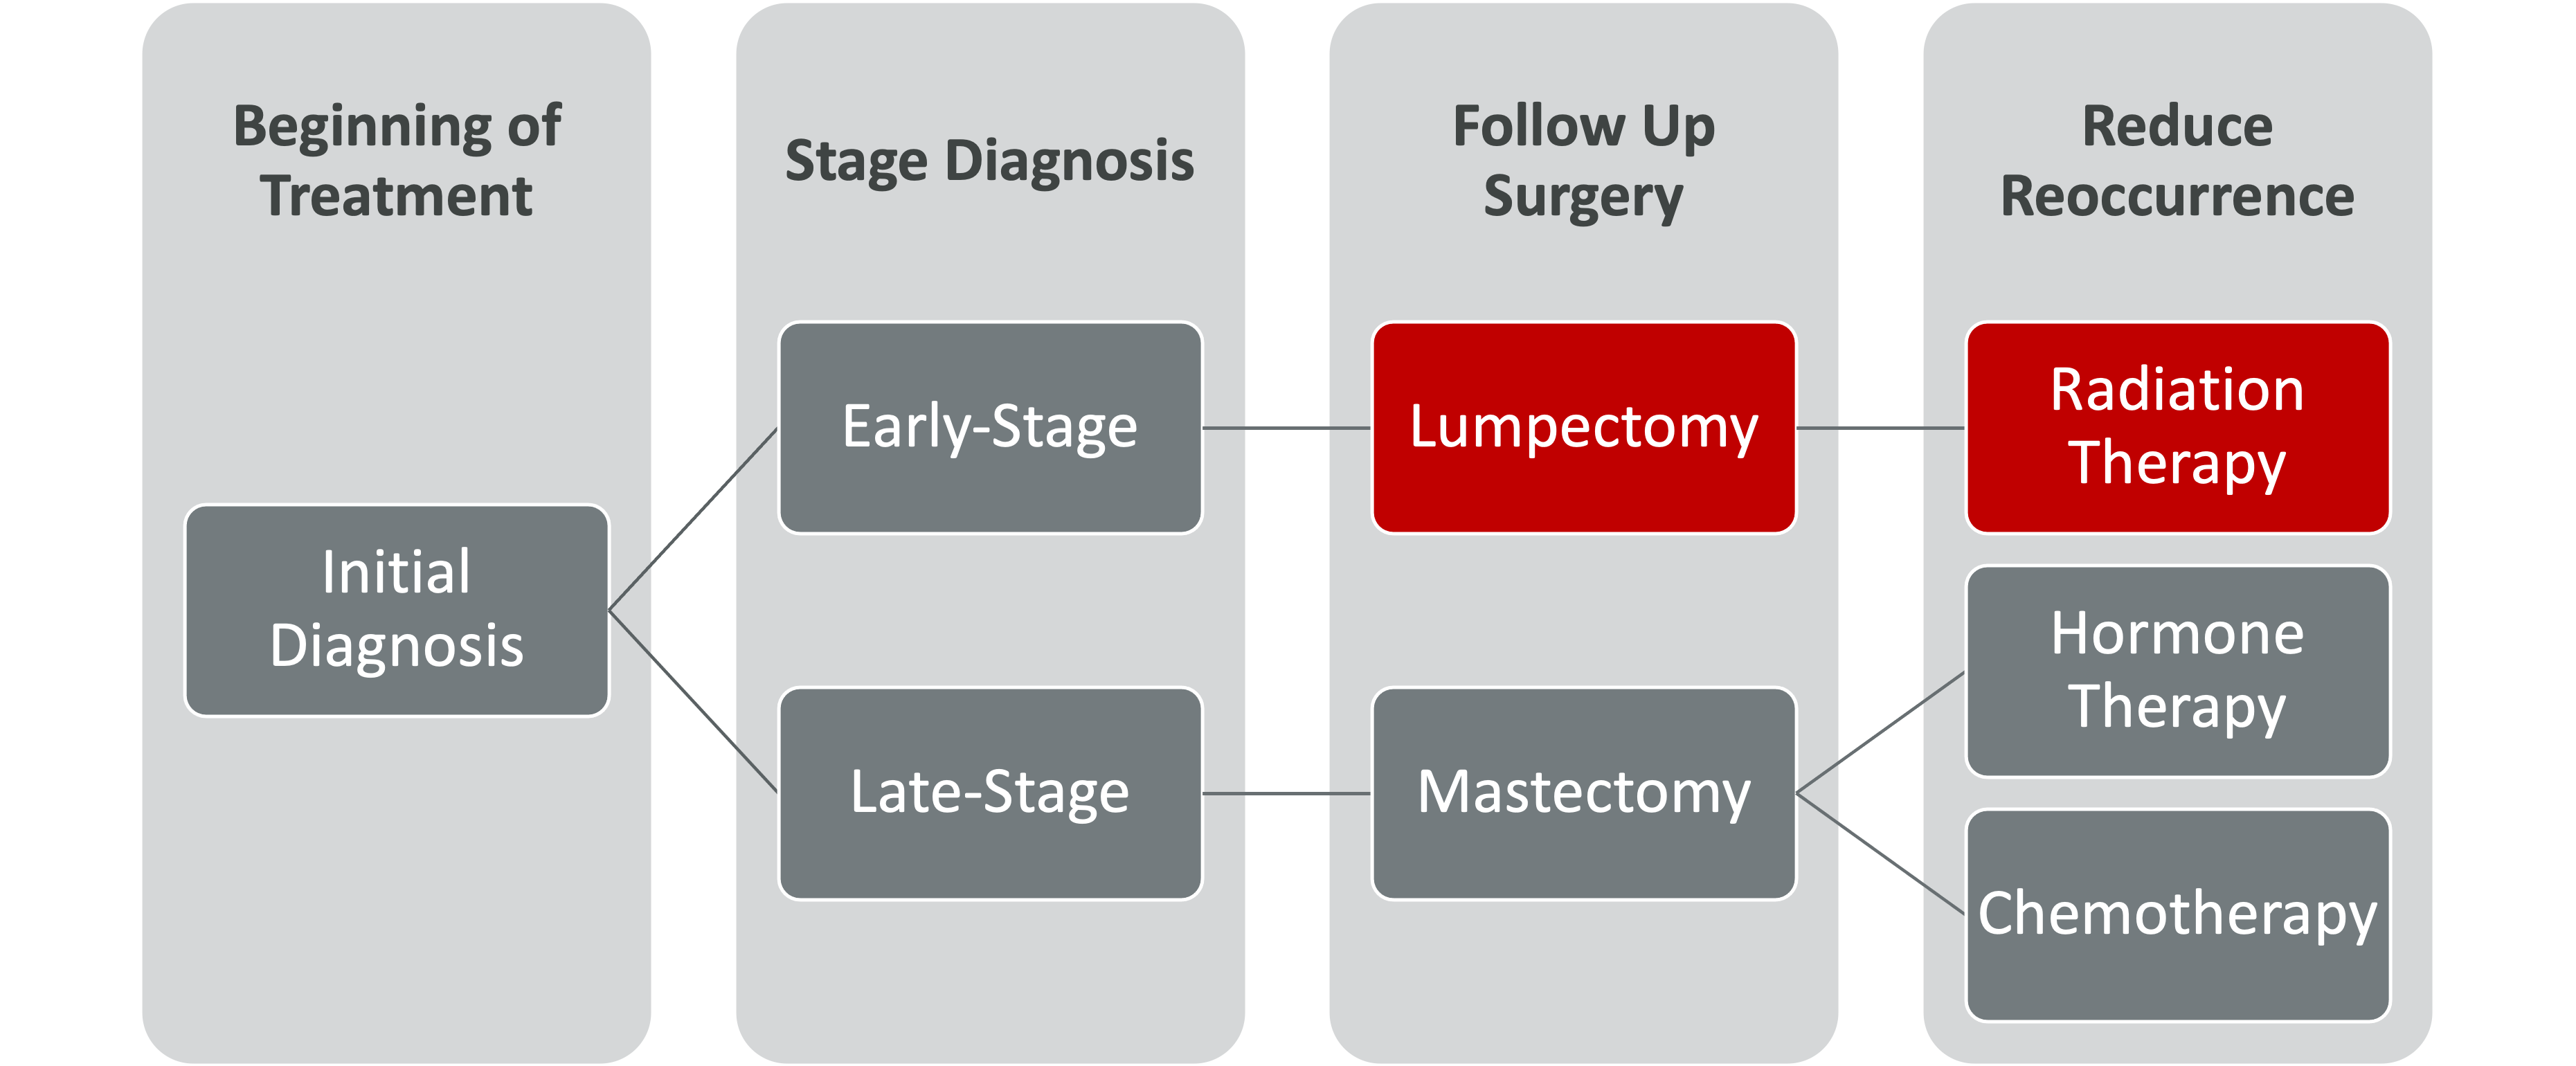
\includegraphics[width=0.6\textwidth]{../figs/introduction/breast_cancer_treatment_process_flowchart.png}
        \caption{Breast Cancer Treatment Options Overview \cite{RefWorks:RefID:37-memorialsurgery}, \cite{RefWorks:RefID:370-einsteinisaac}.}
        \label{fig:introduction:breast_cancer_treatment_options_overview}
\end{figure}

\subsection{Radiation Therapy\label{sec:introduction:radiationtherapy}}
\subsubsection{Radiation Therapy Overview\label{sec:introduction:radiationtherapy:overview}}
As mentioned in Section~\ref{sec:introduction:breastcancer:currenttreatmentoptions:surgicaloptions}, radiation therapy often follows a lumpectomy procedure to kill any stray cancer cells and prevent the cancer from resurfacing. Together, a lumpectomy procedure followed by radiation therapy is commonly known as breast-conserving therapy (BCT). Some compare breast cancer surgery to picking up the large pieces of a broken glass off the floor, while radiation therapy is like vacuuming the remaining shards at the end.

Including radiation therapy after a lumpectomy has been shown to reduce the risk of ipsilateral (same side) recurrence as well as increase overall survival rates~\cite{RefWorks:RefID:157-thomasscience}, ~\cite{RefWorks:RefID:198-jiao2024interobserver}.

\subsubsection{Whole vs Accelerated Partial Breast Irradiation\label{sec:introduction:radiationtherapy:wholevsacceleratedpartialbreastirradiation}}
Patients undergoing BCT can receive either whole breast irradation (WBI) or accelerated partial breast irradiation (APBI). WBI is the more common of the two techniques, although APBI has been gaining traction in recent years due to its unique benefits~\cite{RefWorks:RefID:157-thomasscience}.

WBI is delivered over the course of five to six weeks while APBI is delivered over the course of one week. APBI also limits radiation exposure to 1-2 cm margin of healthy tissue surrounding the tumor site. This limited exposure reduces radiation exposure risks to surrounding organs such as lungs, heart, or ribs. APBI also resulted in higher rates of "excellent/good" cosmetic outcomes compared to WBI (81\% vs 63\% respectively)~\cite{RefWorks:RefID:157-thomasscience}. Comparison of radiation exposure in WBI vs APBI is illustrated in Figure~\ref{fig:introduction:WBI_vs_APBI_irradiation_comparison}.

\begin{figure}[h!]
        \centering
        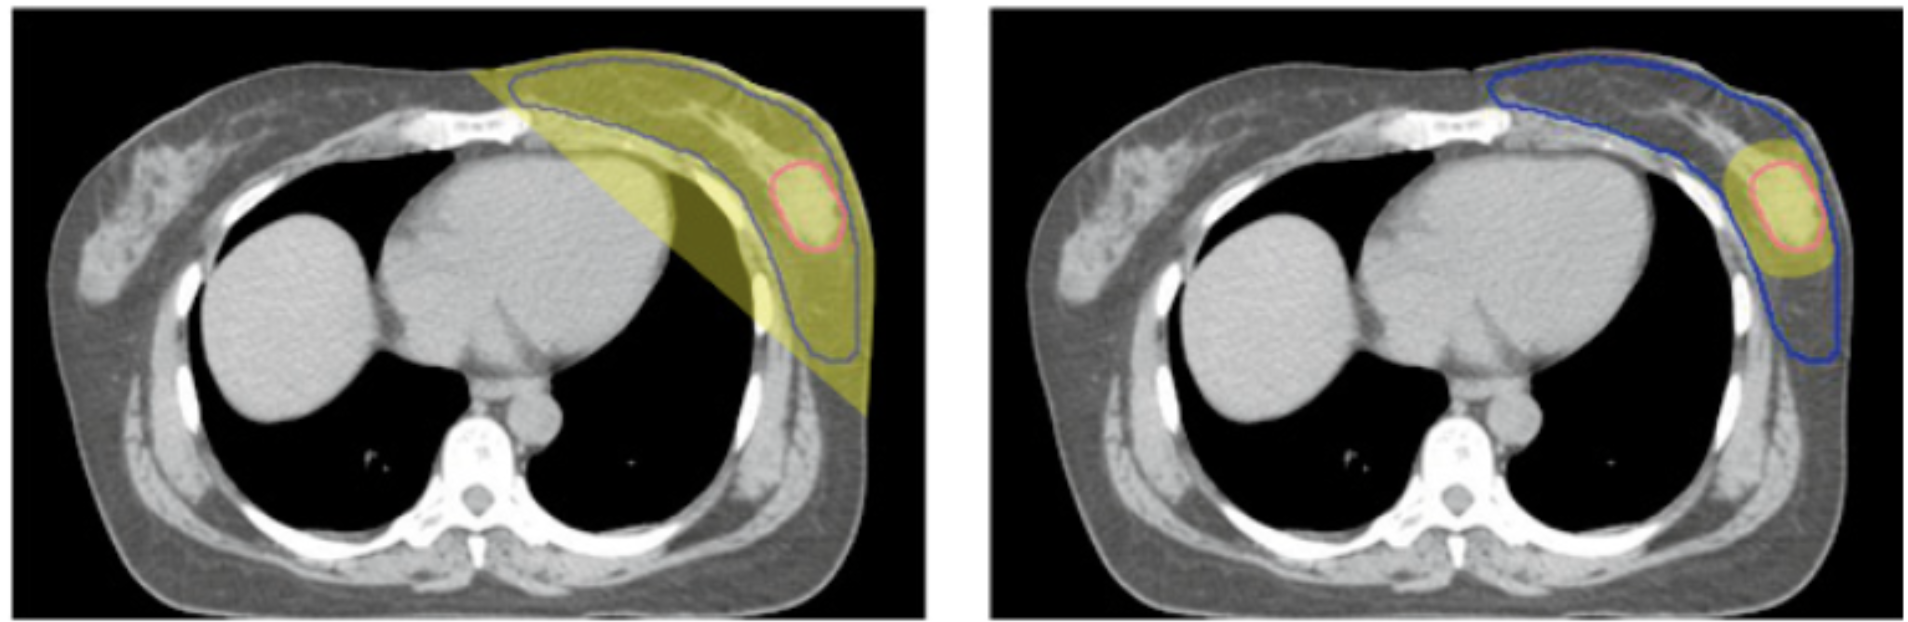
\includegraphics[width=0.6\textwidth]{../figs/introduction/WBI_vs_APBI_irradiation_comparison.png}
        \caption{Comparison of radiation exposure between Whole Breast Irradiation (WBI) (left) and Accelerated Partial Breast Irradiation (APBI) (right) \cite{RefWorks:RefID:157-thomasscience}. The yellow area indicates the irradiated region.}
        \label{fig:introduction:WBI_vs_APBI_irradiation_comparison}
\end{figure}

\subsubsection{Radiation Therapy Treatment Planning\label{sec:introduction:radiationtherapy:treatmentplanning}}
Radiation therapy (WBI or APBI) requires tumor bed delineation to identify and outline the tumor as well as a surrounding healthy tissue margin. This treatment planning ensures radiation is delivered accurately to the tumor site while minimizing exposure to healthy surrounding tissue and organs~\cite{RefWorks:RefID:197-den2015postlumpectomy}.

One concern with tumor bed (TB) delineation is the interobserver variability in accurately marking the TB~\cite{RefWorks:RefID:197-den2015postlumpectomy},~\cite{RefWorks:RefID:179-yang2013tumor}. There are many methods and devices used to assist in TB delineation to address these concerns such as surgical clips, pre-operative imaging, seroma formation, fiducial markers, and other implantable devices~\cite{RefWorks:RefID:179-yang2013tumor},~\cite{RefWorks:RefID:25-acree2022review}.

\subsection{Motivation\label{sec:introduction:motivation}}
The motivation for this work stems from the need to standardize and improve the accuracy and consistency of tumor bed (TB) delineation in radiation therapy following a lumpectomy procedure.

The challenges with accurate TB delineation following a lumpectomy procedure arise because the cancerous tissue has been removed, leaving behind a tumor cavity that is difficult to accurately trace~\cite{RefWorks:RefID:25-acree2022review}. Additionally, unlike other parts of the body, the breast lacks anatomic landmarks to assist with tumor bed delineation~\cite{RefWorks:RefID:344-mitchell2019adaptable}. This need for a marking method is visualized below in Figure~\ref{fig:introduction:need_for_tumor_bed_marker}.

\begin{figure}[h!]
        \centering
        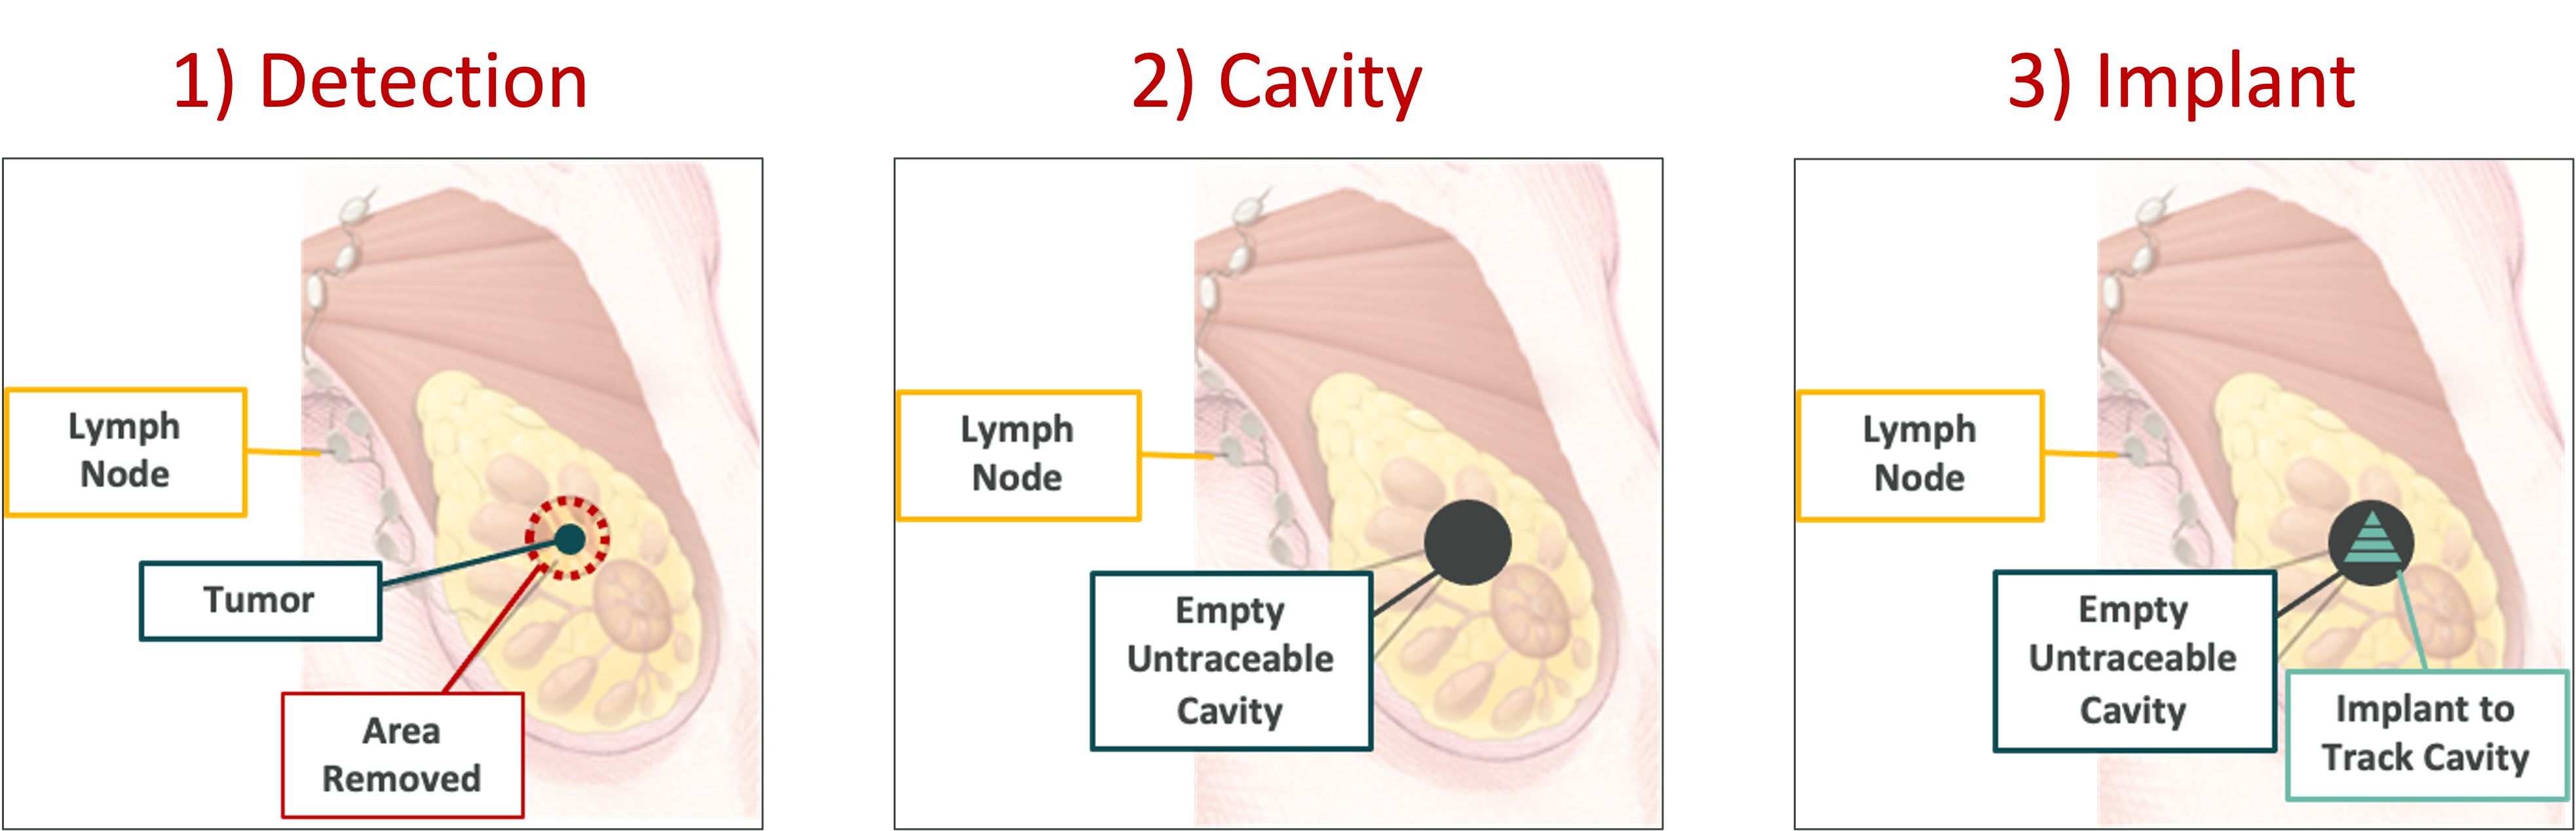
\includegraphics[width=0.6\textwidth]{../figs/introduction/need_for_tumor_bed_marker.png}
        \caption{Motivation for tumor cavity marker following lumpectomy procedure. Adapted from \cite{RefWorks:RefID:38-johnbreastconserving}.}
        \label{fig:introduction:need_for_tumor_bed_marker}
\end{figure}

Current devices and methods used for TB delineation have limitations that affect the overall consistency and accuracy of post-lumpectomy radiation therapy. As over 70\% of breast cancer recurrences occur at the original tumor site, accurate TB delineation and radiation delivery is important in improving patient outcomes~\cite{RefWorks:RefID:25-acree2022review}.

\subsubsection{Importance of Accurate Tumor Bed Delineation\label{sec:introduction:motivation:importanceofaccuratetumorbeddelineation}}
\hl{See if this could use more detail.\\}
Accurate TB delineation is crucial in effective radiation therapy following a lumpectomy procedure given the increasing use of APBI. Since APBI targets a small area of tissue surrounding the tumor bed, accurate delineation is necessary to ensure the radiation dose is delivered precisely to the intended area while minimizing exposure to surrounding healthy tissue and organs~\cite{RefWorks:RefID:197-den2015postlumpectomy}, ~\cite{RefWorks:RefID:25-acree2022review}.

Overestimating TB volume, common in seroma-based delineation, is associated with an increased risk of subcutaneous fibrosis and poorer cosmetic results~\cite{RefWorks:RefID:197-den2015postlumpectomy}. Conversely, underestimating TB volume can lead to insufficient radiation coverage of the tumor bed, increasing the risk of local recurrence~\cite{RefWorks:RefID:198-jiao2024interobserver}. An inaccurate TB volume can
also lead to alteration of management of a radiation boost and completely missing one or more margins of the TB~\cite{RefWorks:RefID:344-mitchell2019adaptable}.

\subsubsection{Current Devices and Methods\label{sec:introduction:motivation:currentdevicesandmethods}}
\hl{See if this could use more detail.\\}
Current devices and methods used for TB delineation include titanium, gold, or liquid fiducial markers/surgical clips, surgeon discretion, seroma formation, or implantable devices~\cite{RefWorks:RefID:25-acree2022review}.

Fiducial markers are solid metal clips inserted around the border of a tumor cavity immediately following the tumor removal~\cite{RefWorks:RefID:358-defining}. These provide a 2D point mapping of the tumor space as shown below in Figure~\ref{fig:introduction:imaging_of_fiducal_clips_in_phantom_breast}.

Liquid fiducial markers were first used as spacers for prostate cancer treatment planning. They have since been repurposed to be used for TB delineation. These markers provide a clearer delineation than solid clips as they conform to the tumor cavity shape~\cite{RefWorks:RefID:25-acree2022review}.

\begin{figure}[h!]
        \centering
        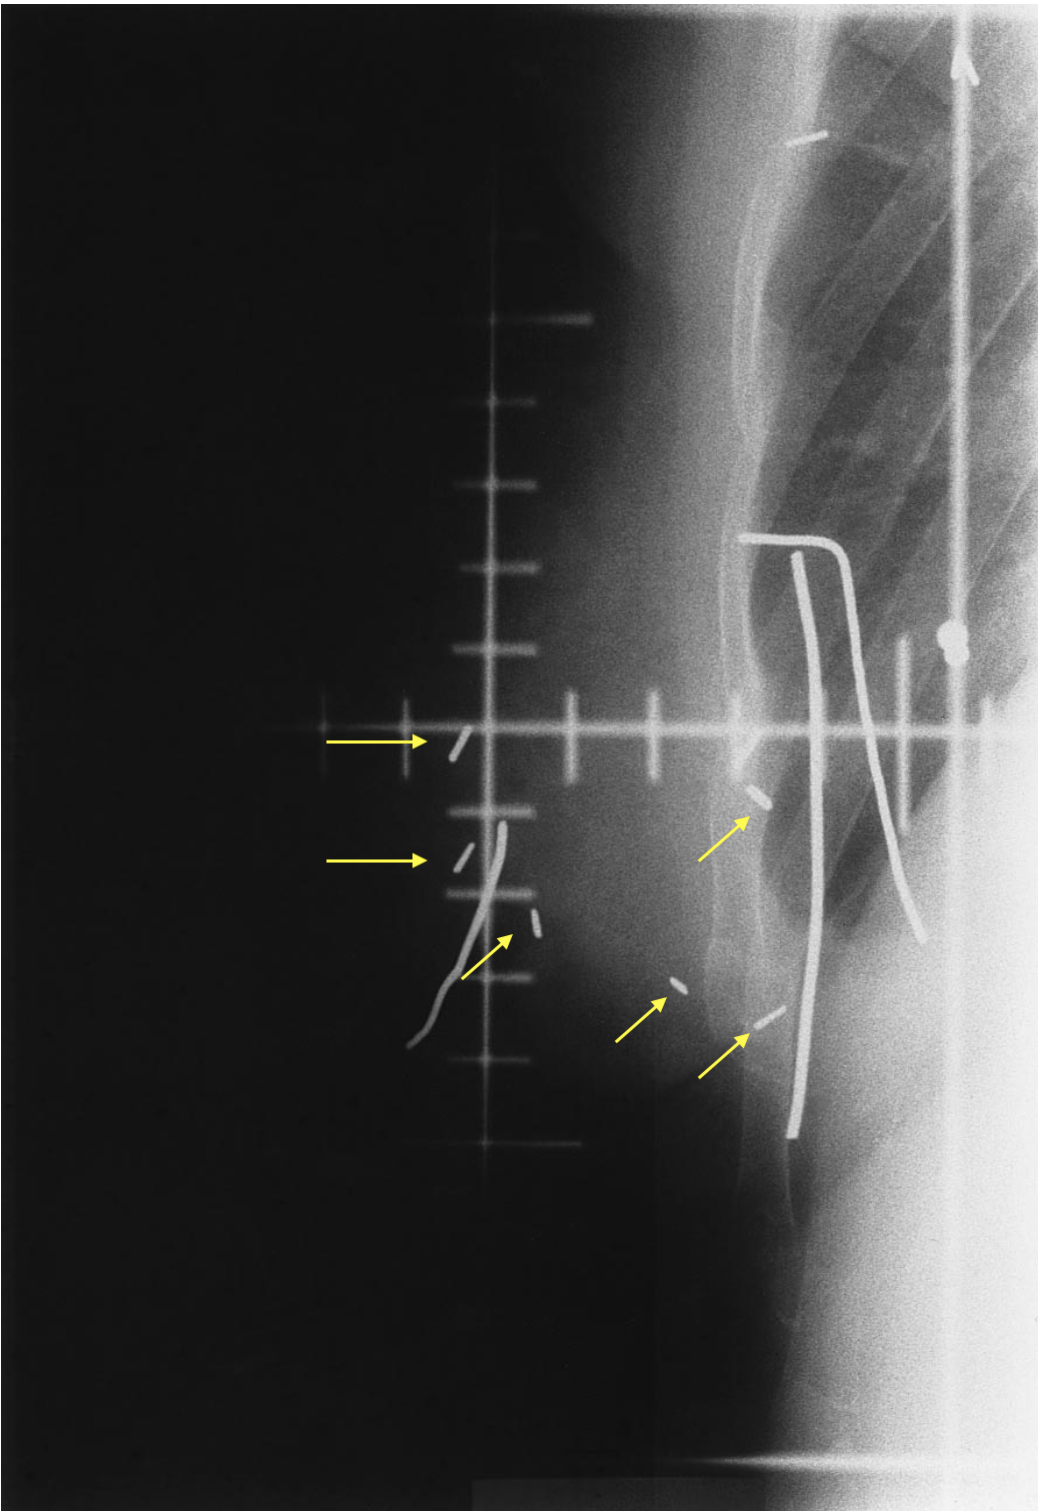
\includegraphics[width=0.6\textwidth]{../figs/introduction/imaging_of_fiducal_clips_in_phantom_breast.png}
        \caption{Imaging of Fiducial Clips in Phantom Breast. Yellow arrows indicate fiducial clips placed around tumor cavity. Adapted from \cite{RefWorks:RefID:178-krawczyk1994importance}.}
        \label{fig:introduction:imaging_of_fiducal_clips_in_phantom_breast}
\end{figure}

Using seroma formation to mark the tumor bed for radiation therapy involves outlining the seroma that forms following a lumpectomy procedure~\cite{RefWorks:RefID:25-acree2022review}.

Lastly, implantable devices can be used to mark the tumor bed. One example is BioZorb (Hologic) which is a 3-dimensional coil-like structure with titanium clips embedded. This device is implanted into the tumor cavity following a lumpectomy procedure and improves on titanium clips alone by creating a 3D outline of the tumor bed. BioZorb was also designed to be reabsorbed into the body within a year~\cite{RefWorks:RefID:25-acree2022review}. BioZorb is shown below in Figure~\ref{fig:introduction:biozorb_implant}.

\begin{figure}[h!]
        \begin{minipage}{0.92\textwidth}
                \centering
                \begin{subfigure}[b]{0.9\textwidth}
                        \centering
                        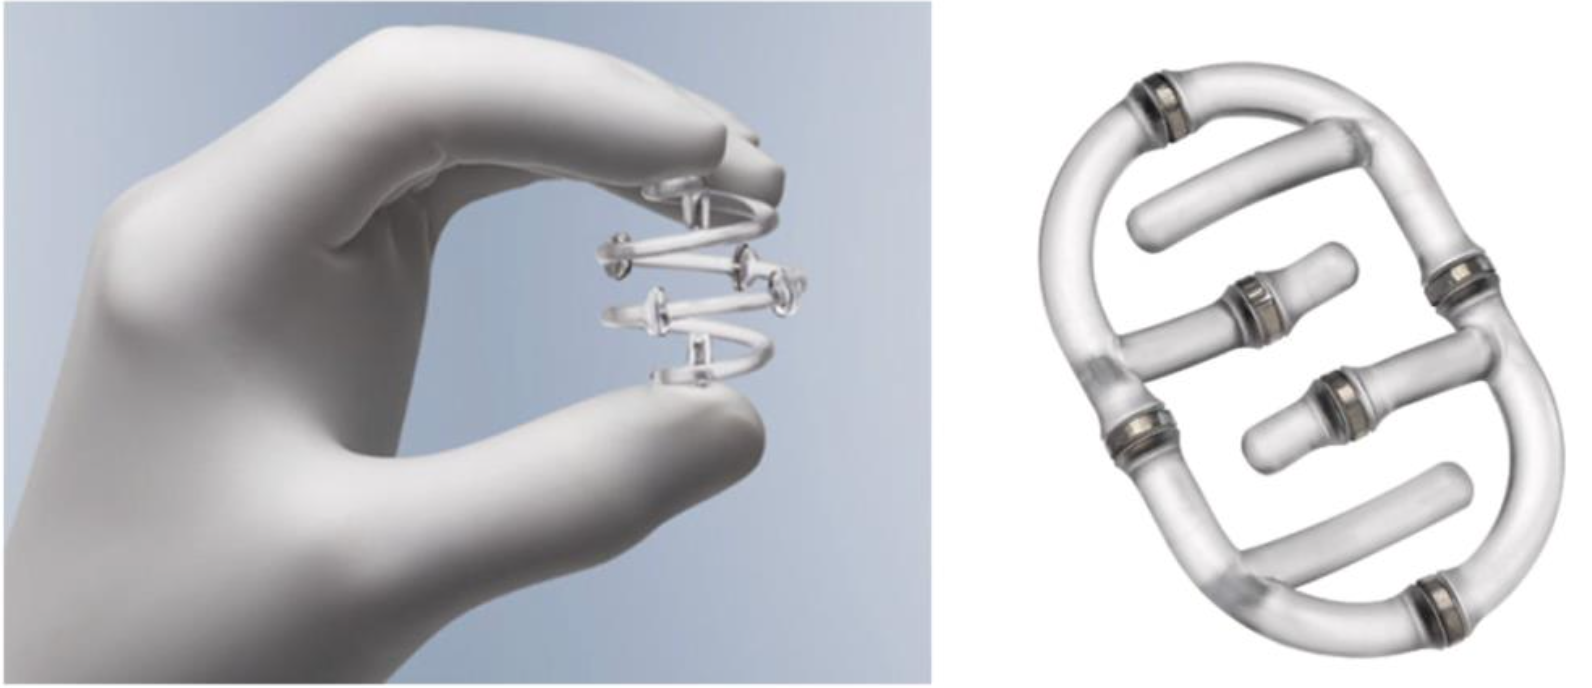
\includegraphics[width=\textwidth]{../figs/introduction/BioZorb_physically.png}
                        \caption{BioZorb physically (top).}
                        \label{fig:introduction:biozorb_physically}
                \end{subfigure}

                \vspace{1em} % optional space between images

                \begin{subfigure}[b]{0.9\textwidth}
                        \centering
                        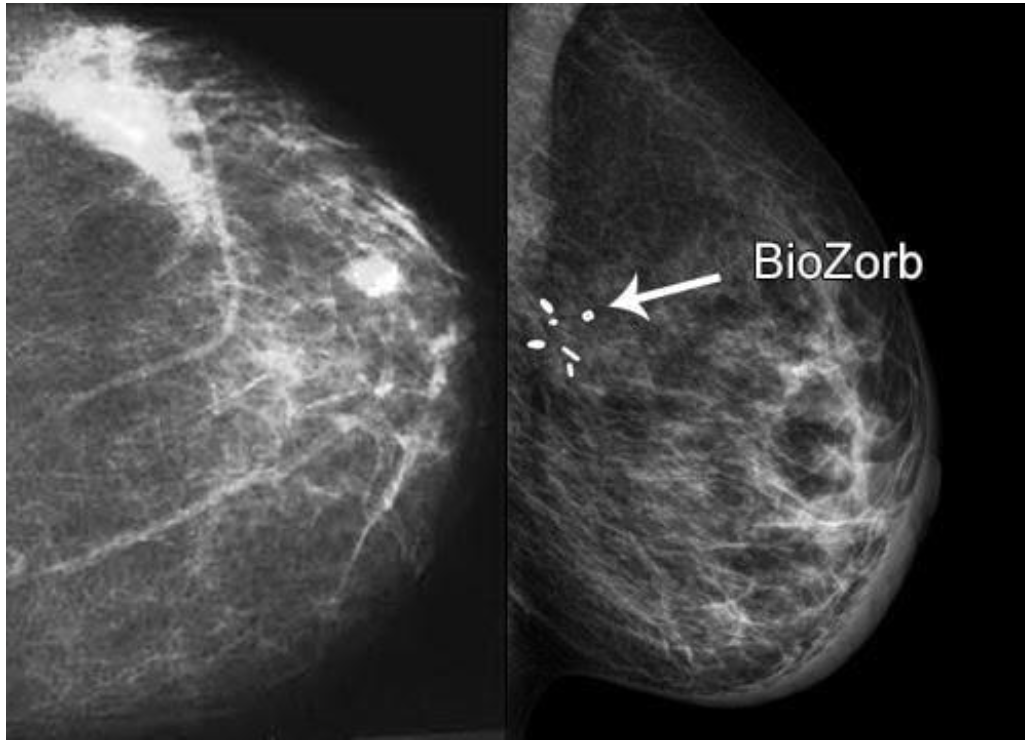
\includegraphics[width=\textwidth]{../figs/introduction/BioZorb_in_imaging.png}
                        \caption{BioZorb in imaging.}
                        \label{fig:introduction:biozorb_in_imaging}
                \end{subfigure}
        \end{minipage}
        \caption{BioZorb, an implantable device to assist with TB delineation~\cite{RefWorks:RefID:370-einsteinisaac}.}
        \label{fig:introduction:biozorb_implant}
\end{figure}

A newer implantable device is Veraform, a continuously radiographically opaque filament that is stitched around the tumor cavity. By being malleable and sewn in place, this device addresses space limitations and migration issues present in other devices~\cite{RefWorks:RefID:344-mitchell2019adaptable}. A simulation showing Veraform in use is shown below in Figure~\ref{fig:introduction:veraform_implant}.
\begin{figure}[h!]
        \centering
        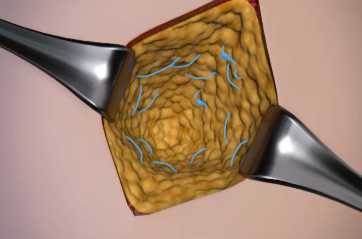
\includegraphics[width=0.6\textwidth]{../figs/introduction/veraform_implant.png}
        \caption{Veraform, an implantable device to assist with TB delineation~\cite{RefWorks:RefID:344-mitchell2019adaptable}.}
        \label{fig:introduction:veraform_implant}
\end{figure}

\subsubsection{Challenges with Current Devices and Methods\label{sec:introduction:motivation:challengeswithcurrentdevicesandmethods}}
\hl{See if this could use more detail.\\}

\subsubsection*{Challenges with Fiducial Markers\label{sec:introduction:motivation:challengeswithcurrentdevicesandmethods:challengeswithfiducialmarkers}}
There are many challenges and inaccuracies that can result from using fiducial markers or surgical clips to create a TB volume. They provide single points of reference which can lead to inaccurate boundaries being drawn, there is no standardized recommendation of how many clips should be used, and clips can migrate over time leading to inaccurate TB localization~\cite{RefWorks:RefID:344-mitchell2019adaptable}. Migration is especially common when patients undergo oncoplastic reconstruction surgery following the lumpectomy procedure. In 2022, it was found the 30,000 breast-conserving therapy patients annually undergo oncoplastic reconstruction surgery~\cite{RefWorks:RefID:25-acree2022review}.

Another concern of surgical clips or fiducial markers is if a re-excision is required. This is when a margin of tissue removed during the lumpectomy is found to contain cancerous cells. When this is the case, a large enough margin surrounding the tumor was not removed, and a re-excision has to be made to remove additional margins. When markers are placed initially, these re-excisions can impact the accuracy of the initial marker placement. It was found that 10\% to 20\% of patients undergoing breast-conserving surgery require a re-excision~\cite{RefWorks:RefID:25-acree2022review}.

\subsubsection*{Challenges with Seroma Formation\label{sec:introduction:motivation:challengeswithcurrentdevicesandmethods:challengeswithseromaformation}}
\hl{Show change in seroma over time visual.\\}

Utilizing seroma formation can be unreliable, as the seroma may not always be localized to the tumor bed, relies on the excision closure method, and time elapsed after surgery\cite{RefWorks:RefID:25-acree2022review}. A seroma may represent the tumor bed, part of the tumor bed, or the entire area in which surgery was performed~\cite{RefWorks:RefID:344-mitchell2019adaptable}.

\subsubsection*{Challenges with Biozorb}
Biozorb was found to provide limited value to patients relative to its high cost~\cite{RefWorks:RefID:344-mitchell2019adaptable}. Additionally, Biozorb was also recalled due to patient discomfort, seroma formation, device migration, and failures to resorb into the body in the designated timeframe~\cite{RefWorks:RefID:296-2024hologic},~\cite{RefWorks:RefID:28-nudelunited}.

\subsubsection{Proposed Solution\label{sec:introduction:motivation:proposedsolution}}
% Explain our research and the proposed mesh


\section{Design\label{chapthree:design}}

\lipsum{}

%%% Local Variables:
%%% mode: latex
%%% TeX-master: "../dissertation"
%%% End:


\section{Implementation\label{chap1:impl}}


%%% Local Variables:
%%% mode: latex
%%% TeX-master: "../dissertation"
%%% End:


\section{Evaluation\label{chap1:eval}}

%%% Local Variables:
%%% mode: latex
%%% TeX-master: "../dissertation"
%%% End:


\chapter{Conclusion\label{chap:conclusion}}

\if@ms
In this chapter, we summarize the status of the work presented in this proposal, and outline future plans~\cite{template}.
\else
In this chapter, we summarize the status of the work presented in this dissertation, and outline future plans~\cite{template}.
\fi

\section{Summary\label{sec:conclusion:summary}}

\lipsum{}

\section{Contributions\label{sec:conclusion:contributions}}

\lipsum{}


    \chapter{Related Work\label{chap:relatedwork}}

In this chapter, we compare our proposed techniques with related work.

\lipsum{}

%%% Local Variables:
%%% mode: latex
%%% TeX-master: "dissertation"
%%% End:

    \chapter{Future Work\label{chap:futurework}}

In this chapter, we present possible extensions and improvements to our proposed techniques.

\lipsum{}

%%% Local Variables:
%%% mode: latex
%%% TeX-master: "dissertation"
%%% End:

    \chapter{Conclusion\label{chap:conclusion}}

\if@ms
In this chapter, we summarize the status of the work presented in this proposal, and outline future plans~\cite{template}.
\else
In this chapter, we summarize the status of the work presented in this dissertation, and outline future plans~\cite{template}.
\fi

\section{Summary\label{sec:conclusion:summary}}

\lipsum{}

\section{Contributions\label{sec:conclusion:contributions}}

\lipsum{}
       % conclusion stuff

    %
    % If you have appendices in your dissertation, you will need the
    % following, else keep it commented. The following appendices are in
    % files called ``app1.tex'', and ``app2.tex'', and they
    % look just like any chapter.
    %

    % \appendix
    % \include{app1}
    % \include{app2}

    \iftoggle{compact-space}{
  \end{small}
}{}

%
% The all important bibliography file at the end of your document!! Use
% the bibstyle you (your department) like in the \bibliographystyle{}
% statement and list the name of your bibliography database file in
% the \bibliography{} statement.  In this example, ``bibfile.bib'' is
% the name of the database.  See the LaTeX manual appendix B for details
% about the bibliography database and BibTeX.
%

% SB: Space hack for bibliography, can't get spacing to work
\iftoggle{compact-space}{
  \begin{footnotesize}
    \begin{spacing}{0.6}
      }{}

      \bibliographystyle{plain}
      \bibliography{reference}

      \iftoggle{compact-space}{
    \end{spacing}
  \end{footnotesize}
}{}

\end{document}


%%% Local Variables:
%%% mode: latex
%%% TeX-master: t
%%% End:
